\documentclass[12pt,paper=A4]{report}
    % XeLaTeX atbalsts
   \usepackage[table]{xcolor}
    \usepackage{fontspec}
    \usepackage{xunicode}
    \usepackage{xltxtra}
    
    % Valodu atbalsts
    \usepackage{polyglossia}
    \setdefaultlanguage{latvian}
    \setotherlanguages{english,russian}
    \usepackage{array}
    % Fonti -- var rakstīt sistēmas fontu nosaukumus
    % Parastais teksta fonts
    \setmainfont[Mapping=tex-text]{Times New Roman}
    \usepackage[framed,numbered,autolinebreaks,useliterate]{mcode}
    % Fonts krievu valodai, kurā ir arī krievu valodas burti
    %\newfontfamily\russianfont{Times New Roman}
    % Šos fontus tālāk izmantos chapter virsrakstos un url'os (lai būtu kirilicas burti)
    \newfontfamily\sffamily{Times New Roman}
    \usepackage{amsmath}
    \usepackage{setspace}
    
    \usepackage{multicol} 
    
    
    % lai varam normāli rakstīt apakšvītras
    \usepackage{underscore}
    % Lai varam iekļaut attēlus
    \usepackage{graphicx}
    \usepackage{float} 
    \usepackage[export]{adjustbox}
    \usepackage{booktabs}
	\usepackage{multirow}
    % Kurā vietā tiks meklēti attēli - relatīvais ceļs attiecībā pret dokumentu
    \graphicspath{{./PNG/}}
    % Ar šiem PDF'ā būs saliktas saites un tām va uzlikt krāsu
    \usepackage{hyperref} 
    \hypersetup{ colorlinks, citecolor=black, filecolor=black,linkcolor=black,urlcolor=black } 

    
    %% Mainīt chapteru izskatu - centrēts un definētais sffamily fonts (skatīt augstāk)
    \usepackage{titlesec}
    \titleformat{\chapter}{\huge\centering\sffamily}{\thechapter}{1pc}{}
    
    %% Pārdēvējam ``Literatūra`` par ``Izmantotās literatūras un avotu saraksts''.
    
    
    %% Atraitņrindiņas un bāreņrindiņas ( widow orphan) vadība
    \clubpenalty10000
    \widowpenalty10000
    
    %% Visādas atkāpes - 1" (2.54 cm) atkāpe jau ir pēc noklusējuma, šeit tikai korekcijas
    %\setlength{\parskip}{1line}
    \setlength{\topmargin}{0cm}
    \setlength{\headheight}{0in}
    \setlength{\headsep}{0in}
    \setlength{\textheight}{22.7cm}
    \setlength{\textwidth}{15cm}
    \setlength{\oddsidemargin}{0.5in}
    \setlength{\evensidemargin}{0.5in}
    %\setlength{\parindent}{0.25in}
    %\setlength{\parskip}{0.25in}
    \usepackage[top=2.0cm, bottom=2.0cm, left=3.5cm, right=2.0cm]{geometry}
    \titlespacing{\chapter}{0pt}{-1\baselineskip}{\baselineskip}
    
    
    %% uzliekam atkāpes arī nodaļu 1. rindkopas 1. rindai  
    \usepackage{indentfirst}
    
    %– augšā, apkšā un no labās malas 20mm, bet kreisajā malā 35mm
    
    
    %Pārnesumiem - ļauj tiasīt lielākas starpas
    \hyphenpenalty=5000
    
    %% Nodaļu un apakšnodaļu numerācija
    \def\thechapter      {\arabic{chapter}.}
    \def\thesection      {\ifx\chapter\undefined{\arabic{section}.}\else  {\thechapter\arabic{section}.}\fi}
    \def\thesubsection   {\thesection\arabic{subsection}.}
    \def\thesubsubsection{\thesubsection\arabic{subsubsection}.}
     \def\thesubsubsubsection{\thesubsubsection\arabic{subsubsubsection}.}
    %\def\theparagraph    {\thesubsubsection\arabic{paragraph}.}
    %\def\thesubparagraph {\theparagraph\arabic{subparagraph}.}
    
    \newpagestyle{main}{\setfoot{}{}{\thepage}}
    \pagestyle{main}
    \assignpagestyle{\chapter}{main}
    
    %% Attēlu numerācija
    \renewcommand{\thefigure}{\arabic{chapter}.\arabic{figure}.}
    \renewcommand{\thetable}{\arabic{chapter}.\arabic{table}.}
    \renewcommand{\theequation}{\arabic{chapter}.\arabic{equation}.}
    
    \usepackage{totcount}
    
    \newcounter{nofappendices}
    \setcounter{nofappendices}{0}
    \regtotcounter{nofappendices}
    \newtotcounter{fignum}
    \def\oldfigure{} \let\oldfigure=\figure
    \def\figure{\stepcounter{fignum}\oldfigure}
    
    \newtotcounter{tablenum}
    \def\oldtable{} \let\oldtable=\table
    \def\table{\stepcounter{tablenum}\oldtable}
    
    
    \newtotcounter{citnum}
    \def\oldbibitem{} \let\oldbibitem=\bibitem
    \def\bibitem{\stepcounter{citnum}\oldbibitem}
    
    
    %\addto\captionslatvian{
    %\renewcommand\bibname{Izmantotās literatūras un avotu saraksts}}
    \renewcommand{\bibname}{} 
    %\renewcommand{\bibname}{References}
    
    
    \usepackage[figure,table]{totalcount}
    %% Sarakstam visus mainīgos
    %% Mainīgie titullapai, defAutors tiek izmantots arī galvojumā
    \def\defAutors{Linda Kalašņikova}
    \def\defAugstskola{Ventspils Augstskola}{\fontfamily{russianfont}
    \def\defFakultate{Informācijas tehnoloģiju fakultāte}
    \def\defSProgrammas{profesionālās bakalaura studiju programmas\\
              ``Datorzinātnes''}
    \def\defStudents{2. kursa studente \\
              \defAutors}
    \def\defMatrikulasNr{14020024}
    \def\defDarbaNosaukums{Daudzkanālu EEG signālu apstrādes pielietojums, izmantojot dziļās apmācības algoritmus}
    \def\defDarbaVeids{Bakalaura darbs}
    \def\defFakultatesDekans{doc. Dr.phys. Māris Ēlerts}
    \def\defZinVaditajs{Dr. sc. comp. Gundars Korāts}
    \def\defGads{2019}
    
    \usepackage[section]{placeins}
    %\usepackage{biblatex}
    %\addbibresource{library.bib}
    \usepackage[labelsep = space]{caption}
    % \addto\captionslatvian{\renewcommand{\figurename}{att.}
    \addto\captionsenglish{%
      \renewcommand{\figurename}{att.}%
      \renewcommand{\tablename}{tabula}%
      }
    
    \usepackage{caption}
    \captionsetup[table]{%
       labelsep=newline,
       justification=raggedleft,
      singlelinecheck=off
    }
    \usepackage{forest}
    
    \tikzset{
    Above/.style={
      midway,
      above,
      font=\scriptsize,
      text width=1.5cm,
      align=center,
      },
    Below/.style={
      midway,
      below,
      font=\scriptsize,
      text width=1.5cm,
      align=center
      }
    }
    \setmainfont{Times New Roman}
    \titleformat{\chapter}{\fontsize{16}{16}\bfseries\centering\sffamily}{\thechapter}{1pc}{}
    \titleformat*{\section}{\fontsize{14}{14}\bfseries\sffamily}
    \titleformat*{\subsection}{\fontsize{14}{14}\bfseries\sffamily}
    \titleformat*{\subsubsection}{\fontsize{14}{14}\bfseries\sffamily}
    \usepackage{pdfpages}
    
    %% Beidzot sākam rakstīt dokumentu
    \begin{document}
    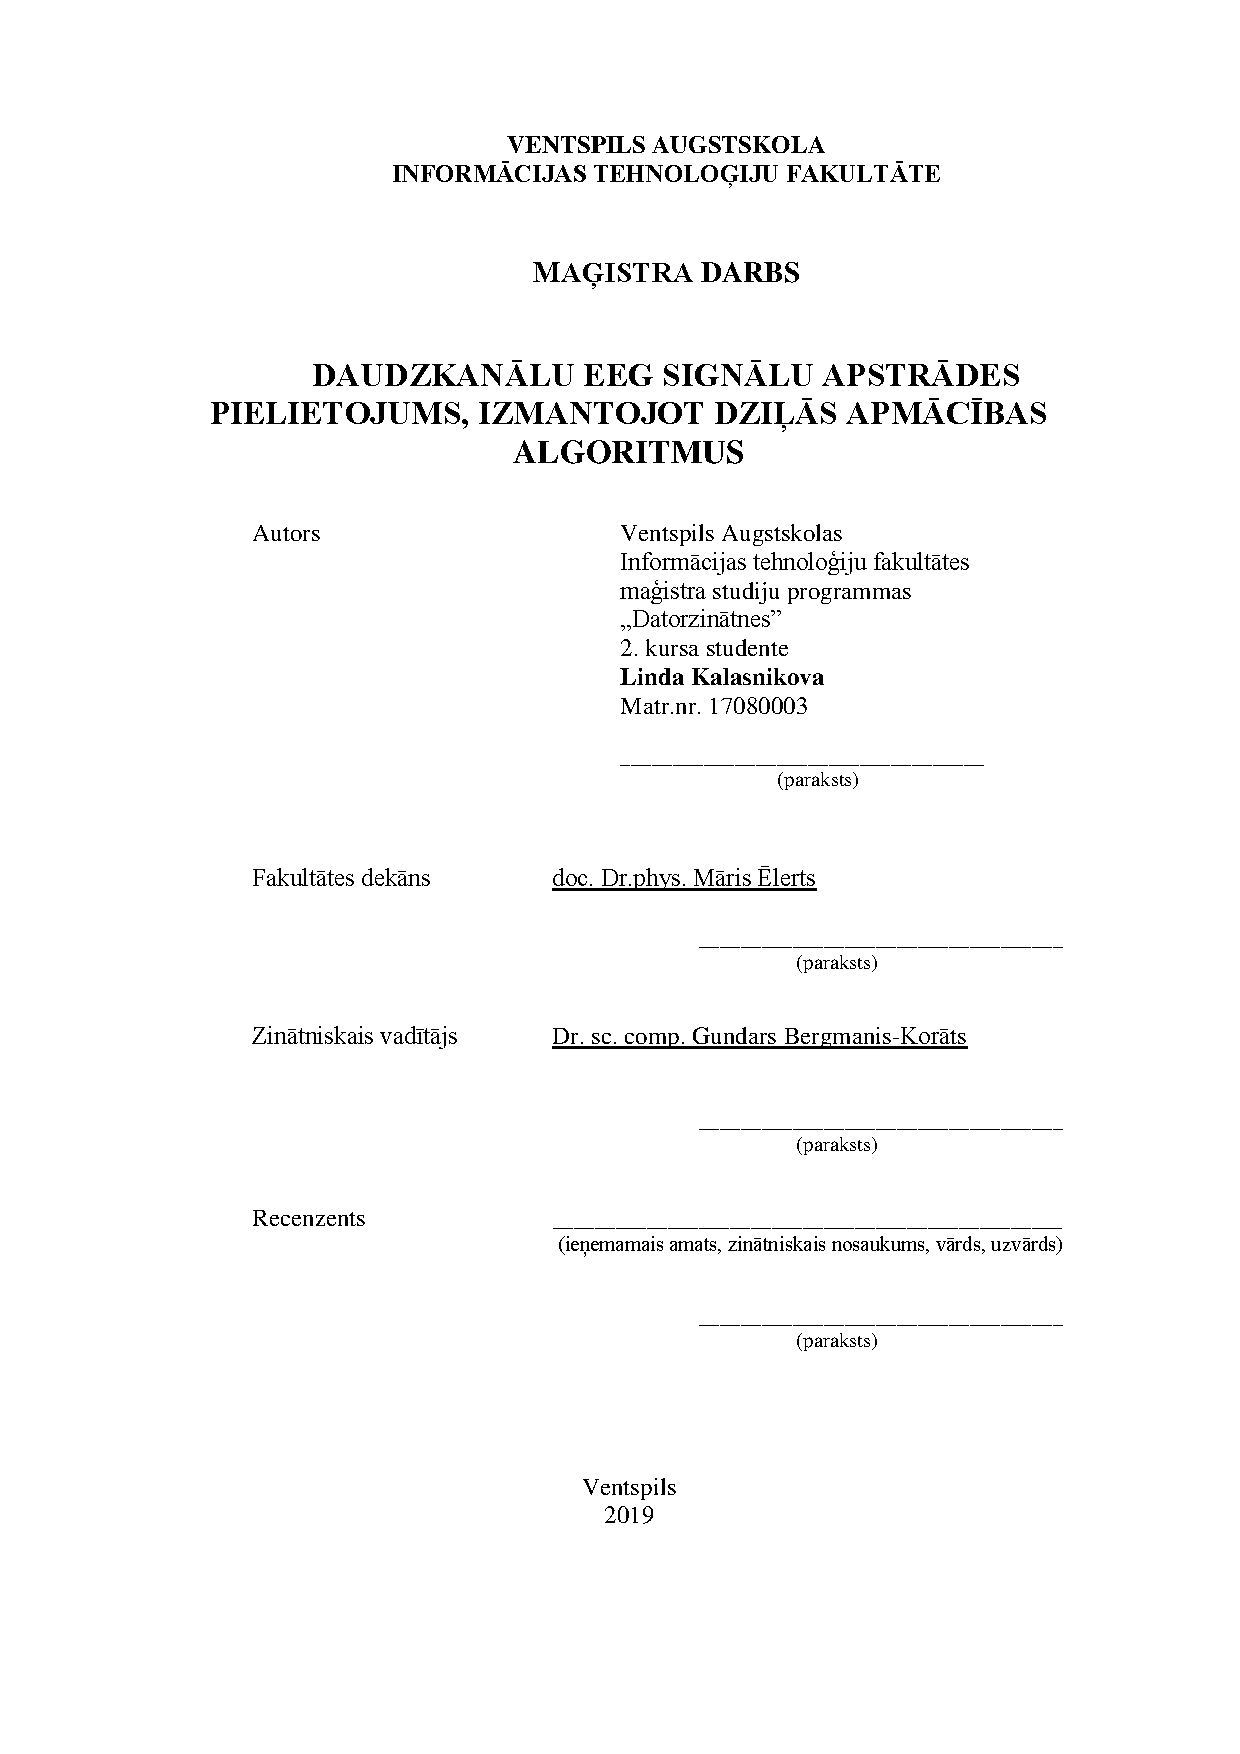
\includepdf[pages=-]{Lindatitullapa.pdf}
    %% Vislabāk nodaļas rakstīt kā atseviškus failus, kurus iekļauj ar input (.tex paplašinājums pats tiek pielikts klāt)
    % \input{mag-titullapa} %% visu titullapu ērtāk ir turēt datnē mag-titullapa.tex, bet te mēs tomēr visu rakstīsim vienā vietā:
    
    %%%% Titullapas sākums
    %\begin{titlepage}
    %\begin{center}
    %\textsc{
    %\defAugstskola\\
    %\defFakultate}\\
    %\vspace{2em}
    %\textbf{\defDarbaVeids}\\
    %\vspace{2em}
    %{\LARGE \textbf{\defDarbaNosaukums}}\\
    %\vspace{2em}
    %\begin{tabular}{@{}r@{}l@{}}
    %\parbox[c]{0.4\textwidth}{Autors:}&
    %\parbox[t]{0.6\textwidth}{
    %\defAugstskola\\\defFakultate\\
    %\defSProgrammas\\
    %\defStudents \\Matrikulas~Nr. \defMatrikulasNr\vspace{0.7em}\\
    %\mbox{}\hrulefill\vspace{-0.4em}\\
    %{\scriptsize(paraksts)}\vspace{2em}} \\
    %\parbox[c]{0.4\textwidth}{Fakultātes dekāns:}&
    %\parbox[t]{0.6\textwidth}{
    %\defFakultatesDekans\vspace{.7em}\\
    %\mbox{}\hrulefill\vspace{-0.4em}\\
    %{\scriptsize(paraksts)}\vspace{2em}} \\
    %\parbox[c]{0.4\textwidth}{Zinātniskais vadītājs:}&
    %\parbox[t]{0.6\textwidth}{
    %\defZinVaditajs\vspace{.7em}\\
    %\mbox{}\hrulefill\vspace{-0.4em}\\
    %{\scriptsize(paraksts)}\vspace{2em}} \\
    %\parbox[c]{0.4\textwidth}{Recenzents:} & \vspace{.7em}\\
    %&\mbox{}\hrulefill\vspace{-0.4em}\\&{\scriptsize(Ieņemamais amats, %zinātn. nosaukums,
    %vārds, uzvārds)}
    
    %\vspace{.7em}\\
    %&\mbox{}\hrulefill\vspace{-0.4em}\\
    %&{\scriptsize(paraksts)}\\
    %\end{tabular}
    %\vfill
    %Ventspils, \defGads
    %\end{center}
    %\end{titlepage}
    %%%% Titullapas beigas
    %Elektroencefalogrāfija    
    %Smadzenes
    	%Smadzeņu aktivitāte
    	%Smadzeņu garozas apgabali
    	%smadzeņu viļņu modeļi
    %Daudz kanālu Elektroencefalogrāfija 
    %EEG veidi %Routine, %Ambulare, %Video, Sleep
    %Sleep EEG 
    	%Miega fāzes
 		%Hypnograms -
 	%Evoked potentials - //can mention what is used for sleep
 	%EEG Mērīšana - EEG norises gaita
 		%Elektrodi - placement, references and bipolar recording
 		%Artefakti 
    	%Abnormal activity
 	%Brain Computer Interface
%Dziļā apmācība
 		%Rekurentie neironu tikli
 			%LSTM
 		%Konvoluciju neironu tīkli
%******************Teoretical Part is over*********************%
		%TO DO stuff

%////////////////////////For Project////////////////////////////// 
	%Elektroencefalogrāfija	
		%smadzenes 		
 			%Apgabali 
 			%vilnju modeļi 
 		%Sleep eeg 
 			%fāzes
 			%hipnogrmmas
 			%evoked potential for sleep EEG
 		%EEG merišana
 			%Elektrodi
 			%Artefakti
 			%Abnormala aktivitate
 	%Dziļā apmācība:
 		%Rekurentie neironu tīkli 
 		%Konvoluciju neironu tīkli
 	%Metodoloģija 
		%Datu kopas sagatave
 		%Tīkla arhitektura 
 			 %LSTM
 			 %LSTM + CNN
 		%Frameworks used - 
 			%python, Kerras, 
 			%Tensorflow
 	%Rezultati un secinajumi
 		
    %%%% Satura rādītājs
    \tableofcontents
    % numeracija ieskaitot titullapu un nonemsana numura no satura
    \setcounter{page}{3}
    \thispagestyle{empty}
    \thispagestyle{empty}
    \addtocontents{toc}{\protect\thispagestyle{empty}}
    %%%% 1.5 līiniju atstarpe starp rindām
    \onehalfspace
    
    %%%% Nodaļa bez numerācijas 
    %%%  Sākas nodaļas
    %\input{ievads} %% Ērtāk visu ir rakstīt atsevišķos failos - ievads.tex un tad tos iekļaut ar input komandu
\chapter*{Anotācija}
\textbf{Darba nosaukums:} Daudzkanālu EEG signālu apstrādes pielietojums, izmantojot dziļās apmācības algoritmus.

\textbf{Darba autors:} Linda Kalašņikova

\textbf{Vadītājs:} Dr. sc. comp. Gundars Bergmanis-Korāts

\textbf{Darba apjoms:} \pageref{LastPage} lpp., \totalfigures\  attēli, \totaltables\ tabulas, \total{citnum}\ bibliogrāfiskās norādes, \total{nofappendices} pielikumi.

\textbf{Atslēgas vārdi:} MIEGA EEG, HIPNOGRAMMA, KONVLOŪCIJA,ILGI-ĪSLAICĪGĀ ATMIŅA.
\vspace{5mm}

Maģistra darba ietvaros tiek apskatīta tēma par smadzenes-dators saskarni (angļu: Brain-Computer Interface), kuras pamatā ir daudzkanālu elektroencefalogrammas (EEG) signālu apstrāde.

Tēma ir aktuāla un nozīmīga pacientiem, kas cieš no miega apnojas. Šis miega traucējums izpaužas kā pēkšņa elpošanas apstāšanās miega laikā.  Miega apnoja ietekmē miega fāzes. Klīnikā tās, savukārt, nosaka vizuāli analizējot elektroencefalogrammas datus. Šī iemesla dēļ ir nepieciešamība pēc automatizēta miega fāžu novērtējuma, kas atļautu veikt miega novērtējumu daudz efektīvāk. 

Pēdējā laikā augstu popularitāti guvušās dziļās apmācības metožu pielietojums sniedz iespēju apstrādāt datus gan industrijā, gan medicīnā. Šī iemesla dēļ maģistra darba ietvaros tiks apskatītas un pielietotas dažādas dziļās apmācības metodes miega fāžu klasificēšanā. 


Eksistē risinājumi (aprakstīti \cite{rahman2018sleep} un \cite{shi2015multi}), kuriem nepieciešama veikt datu priekšapstrādi, lai izgūtu īpašības. Šai problēmai ir arī risinājumi, kuri pielieto dziļās apmācības metodes uz EEG datiem \cite{git1}, \cite{git2}, taču mazo datu dēļ rezultāti nav pietiekoši labi. Tādēļ autore apskata dziļās apmācības modeļus un pieejamos datus, kurus var pielietot modeļu apmācībai.

Darba mērķis ir miega EEG laika rindu mērījumos atpazīt nomoda un miega fāzes. 

Darbā tiek izvirzīti sekojoši uzdevumi, lai sasniegtu mērķi:
\begin{enumerate}
\item Izpētīt pieejamo miega EEG signālu datubāzes.

\item Izpētīt un iepazīties ar esošajiem dziļās apmācības risinājumiem 
laika rindu apstrādē.

\item Izstrādāt metožu un algoritmu kopumu laika rindu signālu klasifikācijā.

\item Sagatavot testa datus algoritmu apmācībai.

\item Veikt modeļu apmācību un analizēt iegūtos rezultātus.
\end{enumerate} 

%Tika secināts, ka uz izvēlēto datu kopu, CNN apvienojot ar LSTM, izdevās iegūt labākus rezultātus nekā izmantojot katru tīklu arhitektūru atsevišķi. Labākā precizitāte, ko izdevās iegūt, ir 63\% pēc CNN-8 - LSTM tīkla optimizācijas. N1 miega stadiju no visām  miega stadijām modeļiem ir visgrūtāk pareizi klasificēt.

\chapter*{Anotation}    

\textbf{Name:}
Multichannel approaches for EEG processing using Deep Learning.

\textbf{Author:} Linda Kalašņikova

\textbf{Supervisor:}
Dr. sc. comp. Gundars Bergmanis-Korāts

\textbf{Workload:} \pageref{LastPage} pages, \totalfigures\ images, \totaltables\ tables, \total{citnum}\ bibliographical references, \total{nofappendices} attachments.

\textbf{Key Words:} SLEEP EEG, HYPNOGRAM, CONVOLUTION, LONG SHORT-TERM MEMORY.
\vspace{5mm}

In Master Thesis will be reviewed topic which is related to the Brain-Computer Interface that is based on the processing of multi-channel electroencephalogram (EEG) signals.

The topic is meaningful and topical for patients suffering from sleep apnea. This sleep disorder is manifested as a sudden stop of breathing during sleep. Sleep apnea affects the sleep phases. In the clinic they are determined by visual analysis of electroencephalogram data. For this reason, there is a need for an automated sleep phase assessment, which would allow for a more effective sleep assessment.

Recently, the use of highly popular deep training methods provides the opportunity to process data in both industry and medicine. For this reason within the Master's thesis, different deep learning methods for classifying sleep stages will be considered and applied.

There are solutions (described in \cite{rahman2018sleep} and \cite{shi2015multi}) that require data pre-processing to retrieve features. There are also solutions to this problem that use deep learning methods on EEG data \cite{git1}, \cite{git2} but due to small data the results are not good enough. Therefore, the author will explore different deep learning models and available data that can be used for model training.

The aim of the work is to recognize wake and sleep stages in Sleep EEG time series measurements.

The following tasks are set to achieve the aim:
\begin{enumerate}
\item Explore available sleep EEG signal databases.

\item Explore and get familiar with existing deep learning solutions for processing time series.

\item Develop a set of methods and algorithms for time series signal classification.

\item Prepare test data for algorithm training.

\item Conduct training, evaluate the obtained results.
\end{enumerate}

%It was concluded that for the selected data set, CNN combined with LSTM, managed to produce better results than using each network architecture separately. The best accuracy you can get is 63\% after CNN-8 - LSTM network optimization. For all tested models N1 sleep stages from all sleep stages is most difficult to classify correctly.


    
\chapter*{Izmantotie saīsinājumi un termini}
\addcontentsline{toc}{chapter}{Izmantotie saīsinājumi un termini}

\textbf{EEG} - Elektroencefalogrāfija (no angļu Electroencephalography)

\textbf{REM} - Ātrās acu kustības (no angļu Rapid eye movement)

\textbf{NREM} - Ne ātrās acu kustības (no angļu Non Rapid eye movement)

\textbf{RNN} - Rekurentie neironu tīkli (no angļu Recurrent Neural Network)

\textbf{LSTM} - Ilgi-īslaicīgā atmiņa (no angļu Long Short-Term Memory) 

\textbf{CNN} - Konvolūciju Neironu Tīkli (no angļu Convolution Neural Network)

\textbf{tanh} - Hiperboliska tangentes funkcija (no angļu Hyperbolic Tangent function)

\textbf{EDF} - Eiropas Datu Formāts (no angļ. European Data Format)

\textbf{MSE} - Vidējā kvadrāta kļūda (no angļ. Mean squared error)

\textbf{1D} - Viendimensionāls

\textbf{2D} - Divdimensionāls

\textbf{3D} - Trīsdimensionāls  

\chapter*{Ievads}
%https://www.ncbi.nlm.nih.gov/pmc/articles/PMC4246141/ -!!!Imoprtant 

%https://thriveglobal.com/stories/this-device-may-be-key-to-finding-out-why-you-arent-sleeping/
\sloppy
\addcontentsline{toc}{chapter}{Ievads}
%http://www.fmed.edu.uy/sites/www.labsueno.fmed.edu.uy/files/9.Diagnostico-polisomnogr%C3%A1fico.pdf
Daudzkanālu signālu apstrāde ir fundamentāla datu analīzes problēma, kas sastopama inženierijas jomās kā, piemērām, dažādās industriālās aplikācijās, tā arī medicīnā \cite{li2011sensor}. 

Šī darba ietvaros tiek apskatīta tēma saistīta ar smadzenes-dators saskarni (angļu: Brain-Computer Interface) ar mērķi miega EEG laika rindu mērījumos atpazīt nomoda un miega fāzes.

EEG signālus pamatā lieto smadzeņu stāvokļa un smadzeņu traucējuma monitoringam un diagnostikai. Taču šādus signālus iespējams izmantot arī smadzenes-dators saskarnē, kur EEG signālos novērotā smadzeņu aktivitāte tiek interpretēta datoram saprotamās komandās.

Tēma ir aktuāla un nozīmīga pacientiem, kas cieš no miega apnojas. Šis miega traucējums izpaužas kā pēkšņa elpošanas apstāšanās miega laikā. Tai ir tendence pasliktināties laika gaitā un dažos gadījumos tā var apdraudēt dzīvību. 
Miega apnoja ietekmē miega fāzes. Klīnikā tās, savukārt, nosaka vizuāli analizējot elektroencefalogrammas datus. Šī iemesla dēļ ir nepieciešamība pēc automatizēta miega fāžu novērtējuma, kas atļautu veikt miega novērtējumu daudz efektīvāk. 

Pēdējā laikā augstu popularitāti guvušās dziļās apmācības metožu pielietojums sniedz iespēju apstrādāt datus gan industrijā, gan medicīnā. Šī iemesla dēļ maģistra darba ietvaros tiks apskatītas un pielietotas dažādas dziļās apmācības metodes miega fāžu klasificēšanā. 

Eksistē risinājumi (aprakstīti \cite{rahman2018sleep} un \cite{shi2015multi}), kuriem nepieciešama veikt datu priekšapstrādi, lai izgūtu īpašības. Šai problēmai ir arī risinājumi, kuri pielieto dziļās apmācības metodes uz EEG datiem \cite{git1}, \cite{git2}, taču mazo datu dēļ rezultāti nav pietiekoši labi. Tādēļ autore apskata dziļās apmācības modeļus un pieejamos datus, kurus var pielietot modeļu apmācībai.

 Rezultātā iegūtās zināšanas un algoritmu pielietojums var tikt pielietots arī citu sensoru datiem, tādējādi radot vērtīgu zināšanu un metožu bāzi pētniecībai un pielietojumiem citās industrijas nozarēs.


Lai sasniegtu darba mērķi nepieciešams veikt sekojošus uzdevumus:
\begin{enumerate}
\item Izpētīt pieejamo miega EEG signālu datubāzes.

\item Izpētīt un iepazīties ar esošajiem dziļās apmācības risinājumiem 
laika rindu apstrādē.

\item Izstrādāt metožu un algoritmu kopumu laika rindu signālu klasifikācijā.

\item Sagatavot testa datus algoritmu apmācībai.

\item Veikt modeļu apmācību un analizēt iegūtos rezultātus.
\end{enumerate}

Maģistra darbs sastāv no 3 nodaļām. 1. nodaļā tiek apskatīts miega EEG un miega fāzes - Nomoda, REM, N1, N2 un N3. 2. nodaļā apskata dziļās apmācības algoritmus, kas sevī ietver Konvolūcijs Neironu Tīklus, Rekurentos Neironu Tīklus un Ilgo Īstermiņa Atmiņu. 3. nodaļā tiek aprakstīta datu kopas sagatavošana, tīklu apmācība, testēšana un rezultātu attēlošana.
    
    %\input{analitiska-dala} %% Ērtāk visu failā analitiska-dala.tex
    \chapter{Miega EEG}  
    Miega EEG ir smadzeņu elektriskās aktivitātes ieraksts, kamēr cilvēks ir  nomoda un miega stāvoklī. Miegs tiek uzskatīts par mainītu vai samazinātas apziņas stāvokli.
    
    Miega EEG tests parasti tiek veikts slimnīcā, izmantojot standarta EEG ierīci \cite{http://www.swbh.nhs.uk/wp-content/uploads/2012/07/What-is-a-sleep-EEG-ML3791.pdf}. Šajā procedūrā izmanto elektrodus, kas reģistrē elektriskā potenciāla izmaiņu uz galvas virsmas pret references elektrodu. Elektrodi tiek novietoti uz galvas ādas. Kā daļu no pārbaudes, var veikt pacienta filmēšanu, lai palīdzētu diagnosticēt slimību. Pirms testa pacients var lietot medikamentus aizmigšanai. Pārbaude ilgst vienu vai divas stundas. Kad pacients ir pamodies, viņš parasti var doties mājās.

Ir dažāda veida miega EEG ieraksti:

\begin{enumerate}
\item \textbf{Bezmiega EEG} - Lai veiktu šo pārbaudi, nepieciešams izvairīties no gulēšanas vai arī gulēt tikai noteiktas stundas naktī pirms testa. Parasti ārsti specificē kādu režīmu pacientam vajadzētu ievērot pirms EEG.
\item \textbf{Dabiska miega EEG} - Lai veiktu šo testu nav nepieciešams īpašs režīms, cilvēks var aizmigt dabiski un nav nepieciešams pirms testa gulēt mazāk nekā parasti.
\end{enumerate}

No EEG izmeklējumiem ir iespējams noteikt smadzeņu viļņu paternus, kas rodas miega laikā un nomodā. Šajos paternos novērojamās izmaiņas var parādīt reģionu, kas ir bojāts un iespējams ir lēkmju rašanās iemesls. EEG var arī uzrādīt pīķus vai asus viļņus, kas liecina par lēkmju risku \cite{epilepsy}. Tā kā tie rodas nejauši, tos var vai nevar redzēt vienā īsā ieraksta laikā.

Procentuāli laiks, ko cilvēks pavada miegā tiek saukts par miega efektivitāti \cite{SleepStagesSecure}. Miega efektivitāti aprēķina, dalot kopējo miega laiku ar kopējo laiku gultā. Miega efektivitāte, kas pārsniedz 90\%, tiek uzskatīta par normālu un optimālu.


    \section{Miega fāzes}
    
    Miega režīms ir sadalīts divos galvenajos miega stāvokļos - ātrās acu kustības un ne ātrās acu kustības stāvoklī. NREM ir sadalīts trīs posmos: N1 fāzē, N2 fāzē un N3 fāzē. N1 fāze tiek uzskatīta par miera pārejas posmu, šo fāzi raksturo īpašības, kuras var novērot gan nomoda stāvoklī, gan miega stāvoklī. 
    
    \subsubsection{Nomoda}
    
    Šajā fāzē muskuļu aktivitāte un izziņas reakcija ir augsta un modrība ir atkarīga no daudziem dažādiem faktoriem. Biežu kustību un muskuļu aktivitātes dēļ EEG signālus var būt grūti lasīt. 
       
    EEG signālus šai periodā raksturo parasti augstas frekvences ar jauktu spriegumu \ref{waves}. Šajā posmā Elektromiogrāfija uzrāda to, ka amplitūdas ir augstas un gaisa plūsma mainās atkarībā no aktivitātes līmeņiem \cite{SleepStageScoring}.
    
     Nomoda fāzei ir raksturīgi alfa viļņu paterni. Alfa viļņus var novērot, tad kad cilvēks relaksējas un atrodas nomoda stāvoklī ar aizvērtām acīm. 
    
    Pamošanās pēc miega sākuma ir laiks minūtēs, kuru pavada cenšoties aizmigt, kad ir sasniegts miega stāvoklis. Šo fāzi bieži vien raksturo zemāks aktivitātes līmenis nekā dienas laikā. Pieauguša cilvēka vidējais miega aiztures laiks ir 10-20 minūtes. 
    
    Nomoda stāvoklis sastāda divas trešdaļas no 24 stundu cikla vai aptuveni 16 stundas dienā \cite{SleepStagesSecure}. Vidēji cilvēks guļ vismaz 90\% no miega perioda, tas ir laiks no miega sākuma līdz pamošanās brīdim. Citiem vārdiem sakot, šai fāzei vajadzētu aizņemt mazāk nekā 10\% no miega perioda. 
          
\subsubsection{Ātrās acu kustības}

    REM fāzi bieži sauc par paradoksālu miegu, jo smadzeņu darbība līdzinās smadzeņu darbībai laikā, kad esam nomodā, bet muskuļi ir paralizēti. Muskuļu tonuss šajā posmā ir ļoti zems. REM fāze miega sākuma posmā parasti ir īsāka un kamēr miega periods turpinās, arī laiks, kas tiek pavadīs R fāzē, palielinās. Miega fāze REM ir saistīts ar atmiņu, izzināšanas spēju un ķermeņa atjaunošanos miega laikā. REM fāzes laikā notiek prāta atjaunošana. Pētījumi liecina, ka atmiņa pasliktinās, kad REM fāze samazinās. 
      
    REM fāzi raksturo galvenokārt ātras acu kustības. Fiziskais REM ir fāze, kad acis ātri pārvietojas uz priekšu un atpakaļ. Tomēr tonizējošajā REM periodā ir diezgan izplatīts tas, ka nav redzamas ātras acu kustības. Zāģveida viļņi elektroenciogrammās ir raksturīga viļņu forma, kas bieži parādās REM fāzē un ir visbiežāk novērojama tieši fiziskajā REM fāzē. 
    
    Citas REM fāzes raksturojošās lietas ir muskuļu atonija, zemsprieguma, jauktas frekvences EEG modelis \ref{waves}, ķermeņa temperatūras samazināšanās, mainītas elpošanas modelis. Ja pacienti ir pamodušies no šī miega posma, viņi bieži vien var atcerēties sapņus.
    
    REM fāze ir apmēram 20-25\% no miega perioda. Bet REM fāze mēdz samazināties, ja rodas miega traucējumi \cite{SleepStagesSecure}.
    
\subsubsection{N1}
   
    N1 fāze ir apmēram 5-10\% no miega perioda. N1 fāzes laikā cilvēkam var būt iespēja dzirdēt, atpazīt un reaģēt uz ārējiem stimuliem. EEG paterni var būt diezgan mainīgi, un tie var strauji novirzīties, tāpēc dažreiz ir grūti tos interpretēt. EEG laikā, kad pacients atrodas N1 fāzē, var novērot salīdzinoši zemu sprieguma modeli ar jauktām frekvencēm un ātru EEG aktivitāti. \ref{waves} \cite{SleepStagesSecure}.  N1 arī sauc par pārejas posmu no nomoda stāvokļa. Bieži vien cilvēku var pamodināt no šī stāvokļa un viņš var pat neapzināties, ka bija aizmidzis. 
    
\subsubsection{N2}     

    N2 fāzi raksturo nedaudz dziļāka miega pakāpe, kurā iespējams saskarties ar miega vārpstām \cite{SleepStageScoring} un K kompleksiem. Miega vārpstas ir unikālas EEG viļņu formas, kas norāda uz ārējo stimulu, piemēram, skaņu bloķēšanu \ref{waves}. K kompleksi ir
asi, viengabalaini vai polifāziski lēni viļņi ar asu negatīva augšupvērstu novirzi, kam seko lēnākā pozitīva lejupvērsta novirze. K kompleksi, pat bez miega vārpstām, ir pietiekams radītājs, lai atpazītu N2 pakāpi. N2 fāzē daudz mazāk apzinās, kas notiek apkārt, nekā tad, kad cilvēks atrodas N1 fāzē. N2 fāze ir apmēram 40-50\% no kopējā miega perioda. 
    
\subsubsection{N3}

   N3 fāze sevī ietver 3. un 4. fāzi. EEG, kad iestājas N3 fāze ir novērojamas mēreni zemas frekvences un liela amplitūdas aktivitāte \ref{waves}. Fāze N3, kas formāli saucas par deltas miegu, tiek uzskatīts par dziļāko miega posmu, jo šajā posmā ir grūti izsaukt jebkādu reakciju \cite{SleepStageScoring}. N3 parasti ir posms, no kura visgrūtāk ir pamodināt cilvēku. Cilvēka pamodināšana no N3 posma bieži izraisa apjukumu un dezorientāciju. N3 fāze ir, apmēram, 20-25\% no miega perioda un dominē nakts pirmajā trešdaļā. N3 fāzei ir tendence ievērojami samazināties ar vecumu. 
    
   \begin{figure}[H] \centering
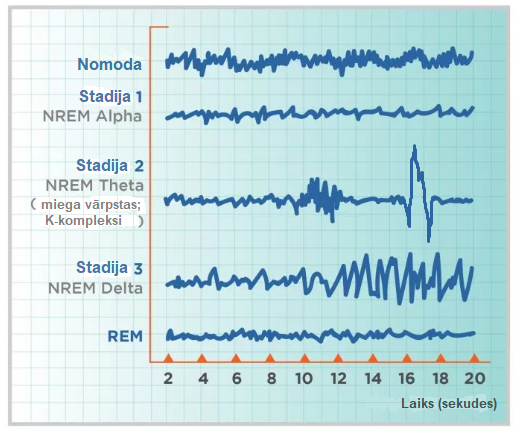
\includegraphics[width=0.50\textwidth]{sleepRecording} 
\caption{Viļņu paterni miega laikā}\cite{seneviratne2017electroencephalography} \label{waves} 
\end{figure}
 
    \section{Hipnogramma}
    Hipnogramma ir polisomnogrāfijas forma jeb grafiks \cite{wiki:xxx}, kas atspoguļo miega posmus kā laika funkciju. Hipnogrammas tika izveidotas, lai vieglāk būtu apskatīt kā elektroencefalogrammas laikā mainās smadzeņu viļņu darbība, kad cilvēks ir aizmidzis. 
    
Hipnogrammas parasti iegūst, vizuāli novērtējot ierakstus no elektroencefalogrammas, elektrookulogrāfijas un elektromiogrāfijas \cite{cabiddu2012modulation}. Šo trīs avotu izejas dati tiek vienlaikus ierakstīti un pēc tam attēloti grafikā kā hipnogramma. 

 Hipnogramma vienā lappusē ļauj attēlot vairākus mainīgos lielumus, ieskaitot miega posmus, elpošanas procesus, pozitīvos elpošanas ceļu spiedienus, mehāniskas kustības, oksimetriju, sirds ritma izmaiņu mērījumus, elektroencefalogrāfijas jaudas spektru un ķermeņa stāvoklis \cite{Hypnogramm}. 
   
Citiem vārdiem var teikt, ka hipnogramma ir visa miega pētījuma saspiests grafiskais kopsavilkums. Hipnogrammas struktūru var apskatīt attēlā \ref{hypnoExample}, kur uz $Y$ ass ir attēlotas miega fāzes un uz $X$ ass laiks, kad sākas un beidzas attiecīgā miega fāze.
     
    Šī darba ietvaros hipnogrammas dati tiks izmantoti, lai veiktu ierakstīto EEG signālu sadalīšanu pa apakš signāliem, kur katrs apakš signāls atbilst konkrētai miega fāzei, tādējādi būs iespējams noteikt kādā fāzē, konkrētā laika brīdī, atrodas cilvēks. Iegūtā datu kopa tiks izmantota neironu tīklu apmācībai un testēšanai.
    
\begin{figure}[H] \centering
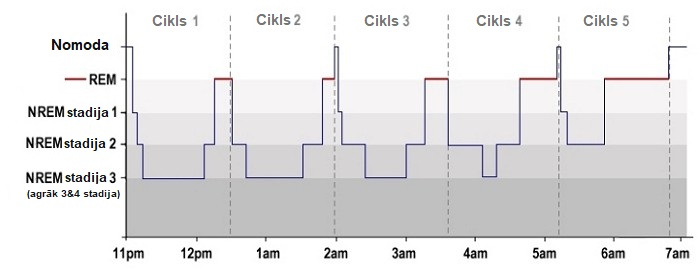
\includegraphics[width=0.70\textwidth]{sleepHypno} 
\caption{Hipnogramma ar miega ciklu sadalījumu} \cite{thebrain} \label{hypnoExample} 
\end{figure}

 \chapter{Dziļā apmācība}
Mašīnmācīšanās (no angļ. Machine Learning) pēta algoritmus un statistikas modeļus, kurus datorsistēmas izmanto, lai efektīvi veiktu konkrētus uzdevumus. Mašīnmācīšanās pamatnoteikums ir veidot algoritmus, kas var saņemt ievades datus, izmantot statistisko analīzi un prognozēt izvades datus bez specifiskas modeļa programmēšanas. Mašīnmācīšanās metodes tiecas iemācīties datos esošo struktūru, tādējādi pielāgojot modeli datu modelim. Ja modeļiem tiek padoti jauni dati, tie spēj patstāvīgi iemācīties jaunajos datos esošo struktūru.

Dziļā apmācība ir specifiska mašīnmācīšanās joma, kurā tiek izstrādātas metodes un algoritmi, kas ļauj no datiem izgūt īpašības un tās tiecas iemācīties datos esošu struktūru (patterns) \cite{lecun2015deep}. Dziļā apmācība atklāj sarežģītas struktūras lielās datu kopās, izmantojot atpakaļ izplatīšanās algoritmu, lai noteiktu kā nepieciešams mainīt tīkla parametrus, lai iegūtu īpašības, kas reprezentē ievades datus. 
	
Pēc Dziļie konvolūcijas tīkli tiek veiksmīgi izmantoti attēlu, video, runas un audio apstrādē, savukārt rekurentie tīkli tiek izmantoti secīgu datu klasifikācijā, piemēram, teksta, runas, video un laika rindu klasifikācijā, notikumu noteikšanā, u.tml.

% \chapter{Tīkla arhitektūras}	
	
\section{Konvolūciju neironu tīkli}

Pēdējo desmit gadu laikā Konvolūciju neironu tīklu pielietojums kļuvis populārs vairākās jomās, kas saistītas ar paraugu atpazīšanu. Tas ietver attēlu apstrādi un balss atpazīšanu. Šis sasniegums ir mudinājis gan
pētniekus, gan izstrādātājus pievērsties lielākiem modeļiem, lai atrisinātu sarežģītus uzdevumus, kas nebija iespējami ar klasiskajiem neironu tīkliem \cite{chen2018rise}.

Konvolūcijas neironu tīkls (no angļ. Convolutional Neural Network) ir dziļas apmācības algoritms, kas var kā ieejas datus izmantot, piemēram, attēlus un piešķir nozīmi (apmācāmus svarus un nobīdes) atsevišķiem attēla aspektiem vai objektiem un tādā veidā algoritms spēj atšķirt vienu no otra. 

CNN prasa daudz mazāku datu priekšapstrādi, salīdzinot ar citiem klasifikācijas algoritmiem. Izmantojot primitīvas metodes filtri tiek manuāli sagatavoti, bet CNN gadījumā pats algoritms spēj apgūt šos filtrus jeb īpašības. Kā arī, izmantojot atbilstošus filtrus, CNN spēj veiksmīgi uztvert datu telpiskās un laika atkarības. 


\subsection{Arhitektūra}

Konvolūciju tīkls sastāv no trīs veida slāņiem. Konvolūcijas slāņa (no angļ. convolution layer), apvienošanas slāņa (no angļ. pooling layer) un pilnībā savienotā slāņa (no angļ. fully connected layer). Var apskatīt attēlu \ref{arherg}, kur tiek parādīta CNN arhitektūra ar daudz avotu sensoru signāliem, kā ievad datiem. Konvolūcijas tiek veiktas sensoru signāliem gar laika asi. Tā kā sensora signāli ir viendimensijas, tiek veikta 1D konvolūcija nevis 2D. Atšķirību var apskatīt attēlā \ref{1dconv}. Pēc tam katra signāla avota apgūtās īpašības tiek apvienotas un izmantotas kā ieejas dati pilnībā savienotajam slānim. Tālāk tiks dziļāk apskatīts katrs no slāņiem. 

\begin{figure}[H] \centering
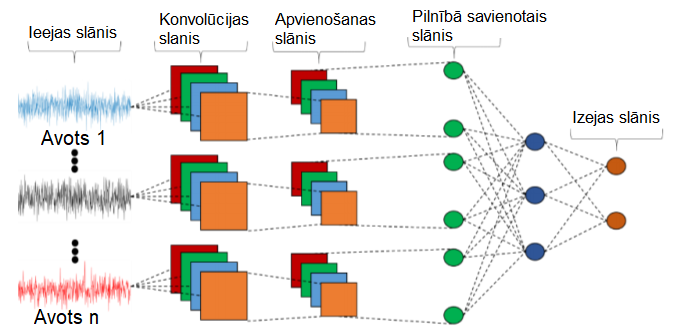
\includegraphics[width=0.70\textwidth]{humanCNN} 
\caption{Konvolūciju neironu tīkls ar daudz avotu senosoru ieejas datiem, kas sastāv no konvolūcijas, apvienošanas un pilnībā savienotajiem slāņiem.}
\cite{inproceeding12}
\label{arherg} 
\end{figure}


\subsubsection{Konvolūcijas slānis}
Kad dati nokļūst konvolūcijas slānī, slānis bīda katru kodolu (filtru) pāri ieejas datu telpiskajai dimensijai, lai izveidotu aktivācijas karti. Šajā gadījumā tiek pielietota nevis 2D konvolūcija, kā attēlu gadījumā, bet gan 1D konvolūcija. Galvenā atšķirība ir ievades datu dimensija un tas, kā filtrs bīdās pāri datiem un to var redzēt attēlā \ref{1dconv}.

\begin{figure}[H] \centering
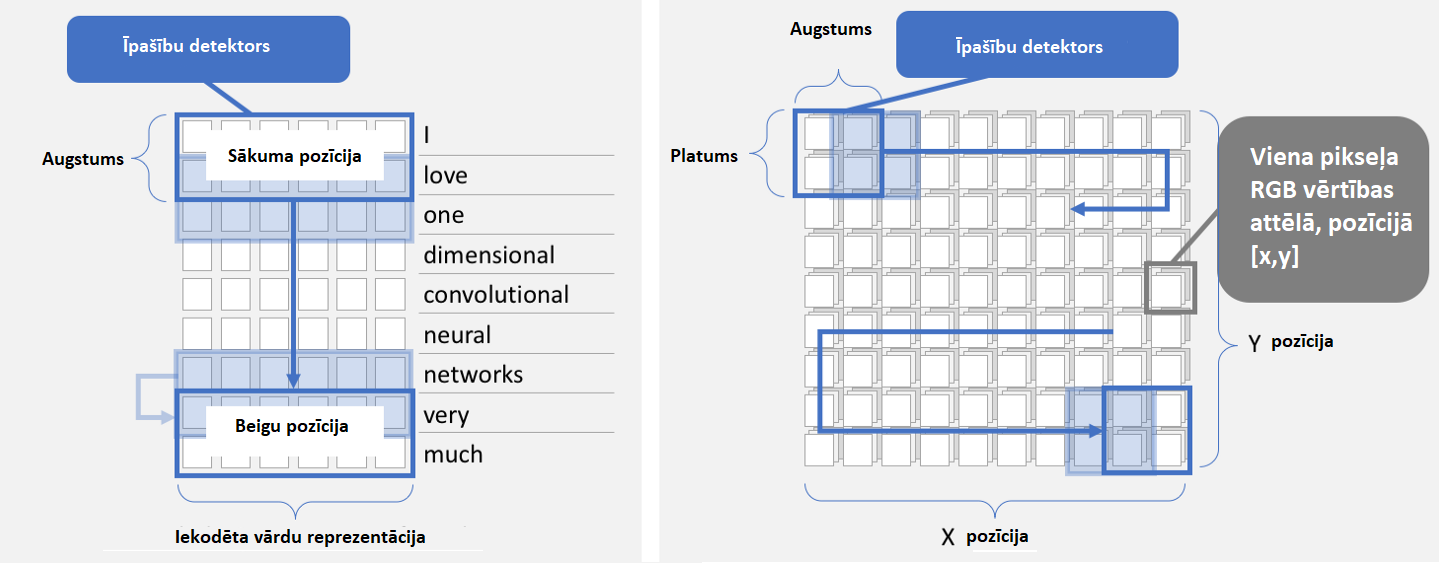
\includegraphics[width=1.00\textwidth]{1DConv} \caption{Pa labi 2D konvolūcijas piemērs ,kur 2x2 filtrs tiek bīdīts pa divdimensionāliem datiem un pa kreisi 1D konvolūcijas piemērs, kur filtrs iet cauri vārdu vektoriem ar soli 2} \cite{lim2017rare}  
\label{1dconv} 
\end{figure}

Īpašību kartes(no angļ. Feature maps) jeb aktivācijas karte (no angļ. Activation maps) ir izejas dati, kas tiek iegūti, kad viens filtrs tiek pielietots iepriekšējam slānim. Dotais filtrs tiek bīdīts pa visu iepriekšējo slāni, vienlaicīgi pārvietojoties pa vienam pikselim. Katra pozīcija izraisa neirona aktivāciju un izejas dati tiek apkopoti aktivizācijas kartē. Kā piemēru var apskatīt \ref{11DovExample}, kur filtru ar izmēru 3 tiek piemērots 1x6 ievades matricai, lai iegūtu izejas datus ar izmēru 1x4. 

%https://machinelearningmastery.com/timedistributed-layer-for-long-short-term-memory-networks-in-python/
%https://machinelearningmastery.com/how-to-get-started-with-deep-learning-for-time-series-forecasting-7-day-mini-course/

\begin{figure}[H] \centering
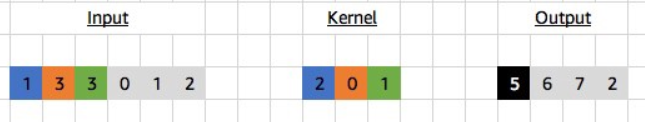
\includegraphics[width=0.70\textwidth]{1DConvCorrect2V} 
\caption{1D konvolūcija.}
\cite{cvbae}  \label{11DovExample} 
\end{figure}

Konkrētais filtrs ar lielumu 3 tiek izmantots, lai aprēķinātu vienu izejas vērtību. Šajā gadījumā, tiek aprēķināts ievades datu un filtra skalārais reizinājums, kas ir tikai attiecīgo elementu reizinājums, kam seko kopējās summas aprēķināšana, lai iegūtu vienu vērtību. Matemātiski tas izskatās šādi \ref{eq:zxc}. 

\begin{equation}
(1 * 2) + (3 * 0) + (3 * 1) = 5
\label{eq:zxc}
\end{equation}

Lai iegūtu pilnīgu izejas datu masīvu $(5,6,7,2)$, izmanto to pašu operāciju, kur izvēlēto kodolu bīda pāri ievades datiem ar soli 1. Atšķirībā no 2D konvolūcijas, kur filtru virza divos virzienos, 1D konvolūcijas gadījumā filtrs tiek bīdīts vienā virzienā - pa kreisi vai pa labi.

Kad filtru bīda pāri ievades datiem, tiek izveidots skalārs produkts, kas tiek aprēķināts katrai filtra vērtībai. Un beigās rezultātam tiek pievienota nobīde. Nobīdes vienība ir papildus neirons, kas pievienots katram pirms izejas slānim un nobīde ir konstanta vērtība 1. Nobīdes vienības nav savienotas ar iepriekšējo slāni un tādējādi neatspoguļo patiesu tīkla aktivitāti. Šīs struktūras mērķis ir noteikt, ka, ja visas neirona ieejas ir 0, tad pēc aktivizācijas funkcijas pielietošanas neironam joprojām būs kaut kādas vērtības.


\begin{figure}[H] \centering
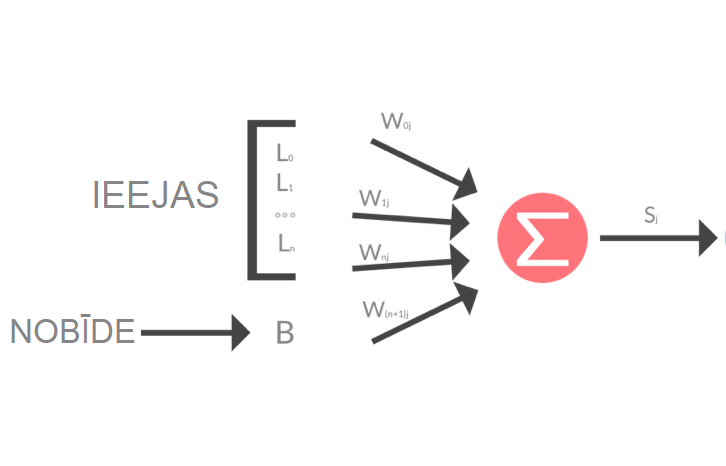
\includegraphics[width=0.40\textwidth]{bias} 
\caption{Neirons ar ievade datiem un saviem svariem, kā arī īpašs ieejas elements - nobīde, kuras vērtība vienmēr ir 1}
\cite{NeuronBia}  \label{bias} 
\end{figure}

Nobīdes vienība tiek pievienota ievades un katra slēptā slāņa sākumā vai beigās, un tas neietekmē iepriekšējā slāņa vērtības. Citiem vārdiem sakot, šiem neironiem nav nekādu ienākošo savienojumu. Nobīdes svaru pievienošanu apraksta ar vienādojumu \ref{eq:biasss}, kur izvades dati $Y$, ievades dati $X$, svari - $W$, $W_b$ nobīde vienības svari..  

\begin{equation}
Y = W * X + W_b
\label{eq:biasss}
\end{equation}

No šīs informācijas tīkls iemācīsies, kuri filtri tiek aktivizēti, kad filtram atrodoties noteiktā pozīcijā ievades datos tiek atrastas attiecīgās īpašības. Šo procesu sauc par aktivizāciju. Katram filtram ir sava atbilstošā aktivizēšanas karte, kura tiek sakārtota atkarībā no dziļuma dimensijas. Katra īpašību karte meklē kaut ko citu. Viena īpašību karte var meklēt taisnas līnijas, otra - līknes. Tādā veidā tiek izveidota pilnīga izvades datu informācija no konvolūcijas slāņa. 

\subsubsection{Aktivizācijas funkcijas}
Neironu tīkls bez aktivācijas funkcijas būtībā ir tikai lineārs regresijas modelis. Aktivizācijas funkcija veic ievades datu nelineāru transformāciju, padarot modeli spējīgu mācīties un veikt sarežģītākus uzdevumus.
Aktivizācijas funkcija ņem vērā mijiedarbību starp dažādiem parametriem un veic datu transformāciju, lai pēc tam izlemtu kuras neironu vērtības pāriet uz nākamo slāni. Eksistē vairākas aktivizācijas funkcijas:

\begin{itemize}
\item \textbf{ReLU} - Pielāgotā lineārā vienība ir visizplatītākā aktivizēšanas funkcija dziļās mācīšanās modeļos. Funkcija atgriež 0, ja tā saņem negatīvus datus, bet ja ir pozitīvas vērtības, tad atgriež šo vērtību $x$ atpakaļ. To var rakstīt ar vienādojumu \ref{eq:ReLU}.

\begin{equation}
f (x) = max (0, x)
\label{eq:ReLU}
\end{equation}

Dēļ negatīvām $x$ vērtībām, gradients var tiekties uz 0. Gradients būs 0 un dēļ tā svari netiks atjaunoti. Tas nozīmē, ka tie neironi, kas nonāk šajā stāvoklī, pārtrauks reaģēt uz kļūdas vai ievades datu izmaiņām. Šo problēmu sauc par mirstošo ReLu.

\item \textbf{Softmax} - Softmax ir ļoti interesanta aktivizēšanas funkcija, jo tā ne tikai ierobežo izejas datu vērtības no datu kopas $X = {x_1,...x_n}$ diapazonā [0,1], bet arī pārveido izvades datus tā, lai kopējā summa būtu 1. Softmax funkcijas \ref{eq:softma} izejas dati atbilst kategoriskajam varbūtību sadalījumam, kas norāda to kāda varbūtība ir katrai klasei.

\begin{equation}
\sigma(z)_j = \frac{e^{z_j}}{\sum^{K}_{k=1} e^{Z_k}}
\label{eq:softma}
\end{equation}

z ir izejas slāņa ievades vektors,
j indeksē izejas vienības, tāpēc j = 1, 2, ..., K.

\item \textbf{Sigmoid} - Šīs aktivizācijas funkcijas \ref{eq:sig} priekšrocība, atšķirībā no lineārās funkcijas, ir tas, ka aktivizēšanas funkcijas izejas dati no padotās datu kopas $X = {x_1,...x_n}$ būs diapazonā (0,1). Tāpēc tas ir īpaši piemērots modeļiem, kuros ir jāparedz, ka izejas dati būs varbūtības. 

\begin{equation}
f(x) = \frac{1}{1+e^{-x}}
\label{eq:sig}
\end{equation}

Virzoties uz abiem sigmoid funkcijas galiem, $Y$ vērtības mēdz reaģēt ļoti minimāli uz $X$ izmaiņām. Un tas var izraisīt to, ka neironu tīkls iestrēgst apmācības laikā. Šī reģiona gradients būs neliels un tas rada izzūdošā gradienta problēmas.

\item \textbf{than} - tanh ir līdzīgs loģistiskajai sigmoidai. Tanh funkcijas \ref{eq:tanh} gadījumā dati no datu kopas $X = {x_1,...x_n}$ tiek ierobežoti diapazonā no -1 līdz 1.  Priekšrocība ir tā, ka negatīvās ieejas vērtības tiks piesaistītas stipri negatīvām vērtībām un nulles ieejas vērtības būs tuvu nullei. Bet, tāpat kā sigmoid funkcijai, tanh ir izzūdošā gradienta problēmas.

\begin{equation}
f(x) = \frac{2}{1+e^{-2x}}-1
\label{eq:tanh}
\end{equation}

\end{itemize}

%https://www.kaggle.com/dansbecker/rectified-linear-units-relu-in-deep-learning
%https://medium.com/the-theory-of-everything/understanding-activation-functions-in-neural-networks-9491262884e0
%formula - https://github.com/Kulbear/deep-learning-nano-foundation/wiki/ReLU-and-Softmax-Activation-Functions

\subsubsection{Hiperparamteri}

Hipersparametru pielāgošana dziļajam neironu tīklam ir sarežģīts process. Hiperparamteri var būt šādi: 

\begin{itemize}

\item \textbf{Mācīšanās ātrums} - Mācīšanās ātrums nosaka, cik daudz optimizācijas algoritmā nepieciešams atjaunot svarus. Var izmantot fiksētu mācību ātrumu, pakāpeniski samazināt mācīšanās ātrumu, paātrinātās metodes vai adaptīvu mācīšanās ātrumu.


\item \textbf{Epohu skaits} - Epohu skaits nosaka to, cik reižu visa treniņu datu kopa iziet cauri neironu tīklam. 

\item \textbf{Partijas lielums} - Partijas lielums nosaka paraugu skaitu, kas tiks izplatīti caur tīklu. Minimālais partijas skaits parasti ir diapazonā no 16 līdz 128.

\item \textbf{Svara inicializācija} - Lai novērstu to, ka neironi mirst, vajadzētu inicializēt svarus ar nelieliem nejaušiem skaitļiem, bet ne pārāk maziem, lai izvairītos no nulles gradienta. Vienmērīgs sadalījums parasti darbojas labi.

\item \textbf{Izslēgšanas metode priekš tīkla regulēšanas} - Kā labu regulēšanas metodi izmanto izslēgšanu, lai izvairītos no tā, ka dziļie neironu tīkli pārmācās. Metode izslēdz no neironu tīkla gadījuma vienības atbilstoši izvēlētajai varbūtībai. Kā sākuma vērtība var izvēlēties 0,5.

\item \textbf{Kodola / filtra lielums} - Filtrs ir svaru matrica, kura tiek bīdīta parī ievades datiem. Konvolūcijas filtrs ir veids, kā atspoguļot īpašības, kuras satur konkrētie ievades dati. Filtru piemērus iespējams apskatīt attēlā \ref{hyperParams}. Filtra matricas svari tiek iegūti, apmācot datus. Mazāki filtri iemācās īpašības, kas ir pēc iespējas lokālākas un lielāki filtri ir vairāk globālām, augsta līmeņa un reprezentatīvai īpašībām. Filtra izmērs parasti ir nepāra.

\item \textbf{Papildināšana} - Papildināšanai (no angļ. padding) parasti izmanto, lai pievienotu papildus kolonnu un rindu ar nulles vērtībām, lai pēc konvolūcijas saglabātu nemainīgus telpiskos izmērus, tādējādi uzlabojot veiktspēju, jo tādā veidā tiek saglabāta informāciju pie robežām. 1D gadījumā nulles var pievienot vektora galos, kā attēlots \ref{hyperParams}. Izejas datu izmērs ir vienāds ar ieejas datu lielumu, to panāk pievienojot papildus datus vienmērīgi pa kreisi un pa labi, bet, ja pievienojamo kolonnu skaits ir nepāra, tas jāpievieno papildus kolonnu pa labi.

\item \textbf{Soļi} - Soļi (no angļ. Stride) parasti ir to pikseļu skaits, kurus vēlaties izlaist, notiekot konvolūcijai, kur ievades datu svaru elementus reizina ar filtra elementiem jeb kamēr filtru bīda pāri ievades datiem horizontāli un vertikāli. To lieto, lai ievērojami samazinātu ieejas datu izmēru. 1D gadījumā filtrs iet cauri vektoram \ref{hyperParams}.

\end{itemize}


%https://www.researchgate.net/publication/324177888_A_Green_Energy_Application_in_Energy_Management_Systems_by_an_Artificial_Intelligence-Based_Solar_Radiation_Forecasting_Model

%https://www.kdd.org/kdd2018/files/deep-learning-day/DLDay18_paper_11.pdf
\begin{figure}[H] \centering
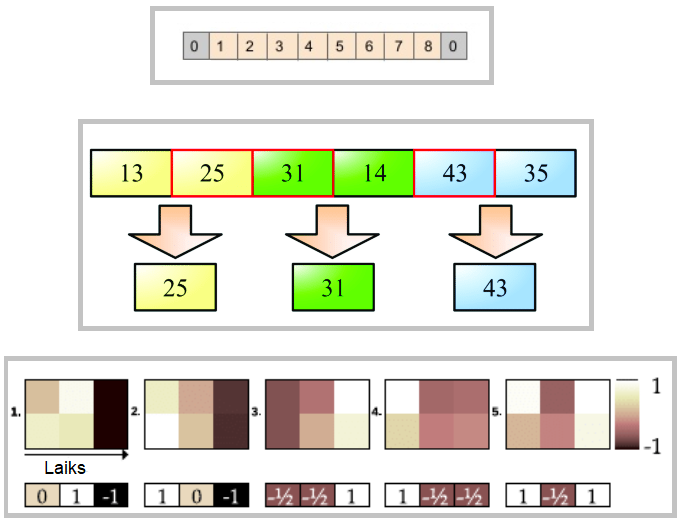
\includegraphics[width=0.70\textwidth]{hyperParams} 
\caption{Pa kreisi augšējā bildē parādīts, kā izskatās nulles vērtības iestatīšana, pa vidu parādīta 1D maksimālā apvienošana, izmantojot soli 2 un apakšējā bildē ir attēloti daži filtri} 
\cite{article123asd} \cite{inproceedings} \cite{1DzerroPadding} \label{hyperParams} 
\end{figure}


\subsubsection{Apvienošanas slānis}

Apvienošanas slāņi tika izstrādāti, lai samazinātu parametru skaitu, kas nepieciešami, lai aprakstītu slāņus, kas ir dziļāk tīklā. Apvienošana arī samazina aprēķinu skaitu, kas vajadzīgs, lai apmācītu tīklu, vai arī, lai vienkārši izpildītu klasifikācijas uzdevuma ne pārāk ilgā laikā.

%Apvienojošie slāņi nodrošina nelielu datu translācijas un rotācijas invariantci \cite{cnnArhVIZRec}. Tomēr tas nenozīmē lielas translācijas vai rotācijas izmaiņas, piemēram, seju, kuru būtu pagriezta par $180°$. Šādus satraucošus traucējumus varēja konstatēt tikai tad, ja oriģinālajā treniņu komplektā bija attēli no sejām, kuru rotācija bija $180°$. Visu iespējamo objekta orientāciju uzskaite prasītu daudz resursu un būtu vajadzīgi vairāk svara parametri.
 
Apvienošanas slāņi ir vērsti uz to, lai pakāpeniski samazinātu dimensiju skaitu, tādējādi vēl vairāk samazinot parametru skaitu un modeļa skaitļošanas sarežģītību. Apvienošanas slānis darbojas ar katru ievades datu aktivizēšanas karti un veic dimensiju mērogošanu, izmantojot, piemēram, $"Max"$ funkciju. Varam apskatīt attēlā \ref{maxPool} aktivizēšanas karti, kurai pielieto maksimālo apvienošanu izmantojot filtru ar dimensionalitāti 2x2. 

\begin{figure}[H] \centering
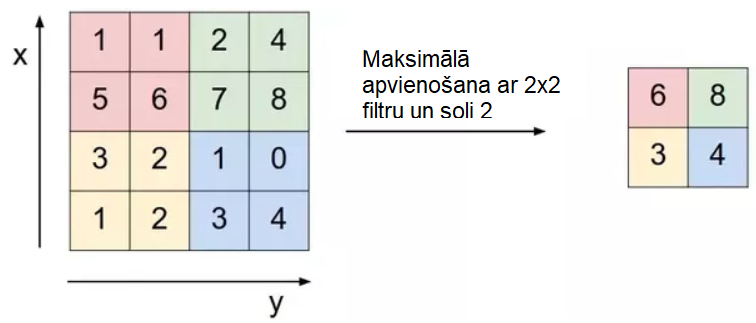
\includegraphics[width=0.40\textwidth]{MaxpoolSample2} 
\caption{Maksimālās apvienošanas operācija} 
\cite{https://medium.com/@RaghavPrabhu/understanding-of-convolutional-neural-network-cnn-deep-learning-99760835f148}  \label{maxPool} 
\end{figure}


    Šo slāni sauc par maksimālais apvienošanas slāni un šajā gadījumā tiek izvēlēta maksimālā vērtība no katras iepriekšējā slāņa neironu kopas. Lielākajai daļai CNN tiek izmantoti maksimālās apvienošanas slāņi ar kodoliem, kuru  dimensionalitāte ir 2x2, kam tiek pielietoti 2 soļi gar ieejas datu telpisko dimensiju. Kā arī notiek aktivizēšanas kartes mērogošana līdz 25\% no sākotnējā datu lieluma. Apvienošanas slāņa destruktīvā rakstura dēļ ir tikai divas maksimālās apvienošanas metodes, kuras izmanto.
     
    Parasti soļi un kodoli tiek iestatīti kā 2 × 2, kas ļaus slānim izstiepties caur ieejas datu telpisko dimensiju. Turklāt var tikt izmantota dublēšanās, kur solis ir iestatīts uz 2, un kodola izmērs ir 3. Destruktīvā rakstura dēļ, ja kodola lielums pārsniedz 3, tas parasti ievērojami samazinās modeļa veiktspēja
     \cite{cnnArhVIZRec}. 
     
\subsubsection{Pilnībā savienotais slānis}     

Tīkla galā tiek pievienots pilnībā savienotais slānis. Pilnībā savienotais slānis satur visus savienojumus ar visām iepriekšējā slāņa aktivācijām, kā redzams regulārajos neironu tīklos. Veids, kādā pilnībā savienotais slānis darbojas, ir tas, ka tas skatās uz iepriekšējā slāņa izvadi un nosaka, kuras īpašības visvairāk atbilst konkrētai klasei un pēc tam tiek izvadītas klašu varbūtības. Pēc tam tiek pielietots atpakaļ izplatīšanās algoritms, lai atjaunotu svarus līdz brīdim, kad tīkls sasniedz kādu noteiktu mazu kļūdas slieksni vai izdara visas iterācijas un apstājas. 

\subsection{Apmācība}

Galvenais apmācību mērķis ir samazināt kļūdu starp prognozētajiem un faktiskajiem datiem. Lai samazinātu kļūdu starp faktiskajiem un prognozētajiem datiem, kļūda tiek atpakaļ izplatīta (no angļ. backpropagate) visos slāņos jeb tiek atjaunināti svari un kad tas ir izdarīts viss process atkārtojas. Shematiski to var redzēt attēlā \ref{propogar}. 

\begin{figure}[H] \centering
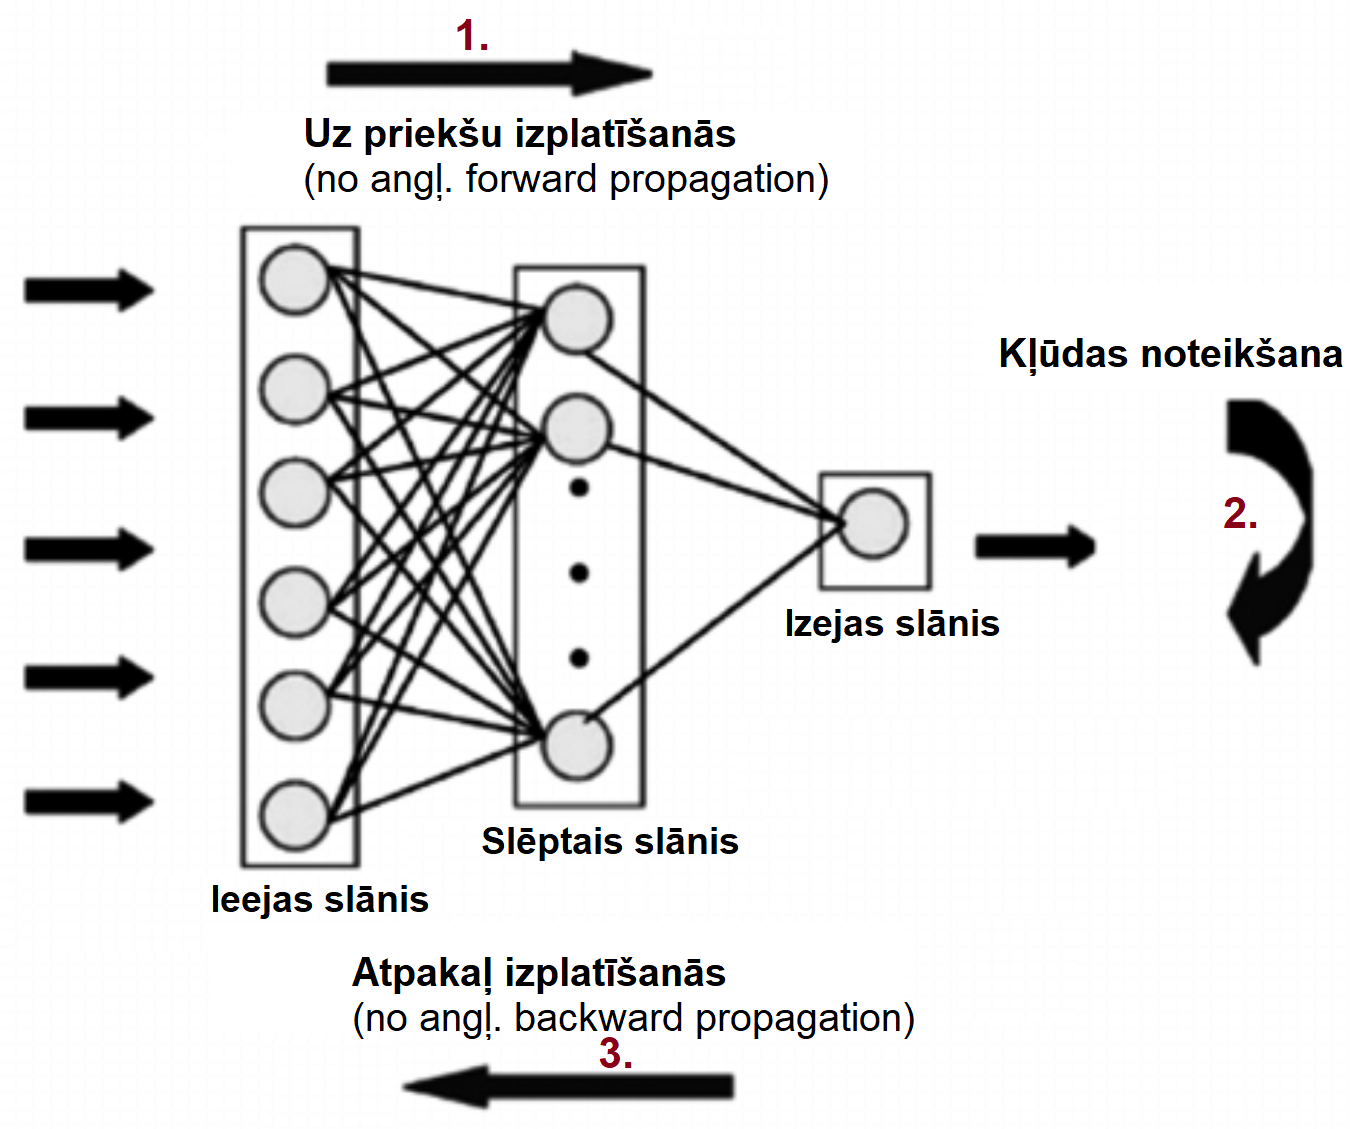
\includegraphics[width=0.70\textwidth]{backpropogateReview} 
\caption{Tīkla apmācības shēma} 
\cite{https://medium.com/coinmonks/backpropagation-concept-explained-in-5-levels-of-difficulty-8b220a939db5}  \label{propogar} 
\end{figure}

Atpakaļ izplatīšanās ir paņēmiens, ko izmanto, lai atjauninātu svarus, izmantojot krītošo gradientu (no angļ. gradient descent). Krītošā gradienta metode ir iteratīvs optimizācijas algoritms, lai atrastu minimālo funkciju. Šajā gadījumā ir jāsamazina kļūdas funkcija (no angļ. loss function), lai atrastu funkcijas lokālo minimumu. Tiek aprēķināts kļūdas funkcijas gradients, kas atkarīgs no neironu tīkla svariem un šis aprēķins turpinās atpakaļ pa visu tīklu. Svari tiek atjaunināti, izmantojot nelielu soli alfa. Vairāk par šo procesu var uzzināt \cite{cui2018applying}.

CNN gadījumā, kad tiek veikta atpakaļ izplatīšanās veidojas papildus grūtības, kas rodas, piemēram, kad nepieciešams veikt atpakaļ izplatīšanos caur apvienošanas slāni.  

Veicot uz priekš izplatīšanos (no angļ. forward propogate) ir nepieciešams saglabāt informāciju par pozīcijām, kurās maksimālajā apvienošanas slānī aktivizācijas kartēm tika noteiktas maksimālā vertības \ref{zeiler}. Atpakaļ izplatīšanās gadījumā visas vietas, kurās neatrodas maksimālā vērtība, tiek iestatītas kā 0, bet maksimālās vērtības vietās tiek iestatīta vērtība 1. Tiek iegūta matrica ar 0 un 1. \cite{https://medium.com/coinmonks/backpropagation-concept-explained-in-5-levels-of-difficulty-8b220a939db5}

Aktivizācijas funkcijas gadījumā arī ir nepieciešams pielietot atpakaļ izplatīšanos. Aktivizācijas karte tiek padota aktivizācijas funkcijai, kas ir, piemēram, ReLU. Tiek iegūta aktivizācijas karte, kur visas negatīvās vērtības tiek aizstātas ar nullēm un to var apskatīt attēlā \ref{zeiler}. Izmantojot ReLU nelinearitātes (no angļ. non-linearities), kas veic aktivizācijas kartes pārveidošanu, tiek nodrošināts tas, ka aktivizācijas kartes vienmēr ir pozitīvas.
 
Tālāk pēc atpakaļ izplatīšanās caur maksimālo apvienošanas slāni un aktivizācijas funkcijas, abu iegūto matricu attiecīgie elementi tiek sareizināti savā starpa (no angļ. element wise multiplication) iegūstot pārveidotu aktivizācijas karti.  

Konvolūcijas slānī, veicot atpakaļ izplatīšanos, CNN izmanto filtrus, kurus tas iemācījās, lai konvolvētu (no angļ. convolve) aktivizācijas kartes no iepriekšējā slāņa. Lai veiktu iznvertāciju, tiek izmantotas to pašu filtru transponētās versijas, bet šie filtri tiek pielietoti iegūtajām pārveidotajām aktivizācijas kartēm nevis zemāk esošā slāņa izeja datiem. Iegūtie rekonstruētie dati parāda visnozīmīgāko informāciju, kas tiek izmantota, lai aktivizētu neironu, kā piemēram, parādīts attēlā \ref{zeiler}. \cite{zeiler2014visualizing} 


\begin{figure}[H] \centering
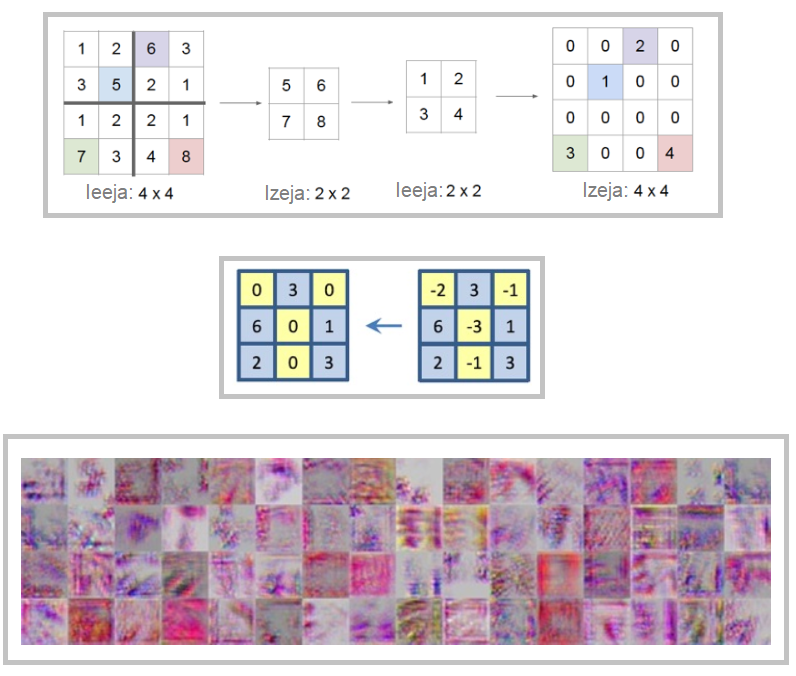
\includegraphics[width=0.80\textwidth]{maxPoolingDDD} 
\caption{Augšējā bilde attēlo atpakaļ izplatīšanos, izmantojot apvienošanas slāņus, vidējā bilde attēlo atpakaļ izplatīšanos, izmantojot ReLU nelinearitātes, apakšējā bilde attēlo iegūtās aktivizācijas kartes pēc atpakaļ izplatīšanās, izmantojot konvolūciju} 
\cite{masdasdIII} \cite{zeilerDed}
 \label{zeiler} 
\end{figure}

%https://medium.com/the-bioinformatics-press/only-numpy-understanding-back-propagation-for-max-pooling-layer-in-multi-layer-cnn-with-example-f7be891ee4b4
%https://srdas.github.io/DLBook/ConvNets.html
%https://datascience-enthusiast.com/DL/Convolution_model_Step_by_Stepv2.html


\subsubsection{Kļūdas funkcijas}
Kļūdas funkcija ir svarīga mākslīgo neironu tīklu daļa, ko izmanto, lai novērtētu neatbilstību starp prognozētajiem izejas datiem un faktiskajām klašu etiķetēm. Kļūdas funkcija ir ne negatīva vērtība, kur modeļa veiktspēja palielinās līdz ar kļūdas funkcijas vērtības samazināšanos. 
Dažas no šīm funkcijām ir: 

\begin{itemize}
\item \textbf{logcosh}. Šī funkcija ir prognozētās kļūdas logaritms no hiperboliskā kosinusa \cite{redDEs}. Un šo funkciju apraksta ar vienādojumu \ref{eq:logCosh}, kur $Y$ apzīmē vektoru ar patiesajām $n$ vērtībām un $\hat{Y}$ apzīmē vektoru ar prognozētajām $n$ vērtībām. $logcosh$ darbojas galvenokārt kā vidējā kvadrāta kļūda, bet to tik stipri neietekmē gadījumi kad ļoti bieži tiek veikta nepareiza izejas datu prognozēšana.

\begin{equation}
L(Y,\hat{Y}) = \sum_{i=1}^{n} log(cosh(\hat{Y_{i}} - Y_i))
\label{eq:logCosh}
\end{equation}

\item \textbf{Kategoriskā starpentropijas kļūda (angļ. val. categorical crossentropy)} To sauc arī par Softmax kļūdu. Šajā gadījumā lieto $Softmax$ aktivizācijas funkciju, kas apvienota ar starpentropijas kļūdu. Šo funkciju izmanto, kad nepieciešams klasificēt vairākas klases. 
Galvenais atcerēties, ka patiesajiem datiem jābūt kategoriskā formātā.

\item \textbf{Vidējā kvadrāta kļūda}
Vidējā kvadrāta kļūda ir visbiežāk izmantotā regresijas kļūdas funkcija. MSE ir kvadrātiskā attālumu summa starp mūsu patiesajiem datiem un prognozētajiem datiem. Un MSE aprēķina pēc formulas \ref{eq:mseE}, kur $Y_i$ ir vektors, kas apzīmē $n$ patieso vērtību skaitu un $\hat{Y_i}$ ir vektors, kas apzīmē $n$ prognožu skaitu. 

\begin{equation}
{\displaystyle \operatorname {MSE} ={\frac {1}{n}}\sum _{i=1}^{n}(Y_{i}-{\hat {Y_{i}}})^{2}}
\label{eq:mseE}
\end{equation}

\end{itemize}
    

    \section{Rekurentie Neironu tīkli}
Rekurentie neironu tīkli (angļ. Recurrent Neural Networks) ir mākslīgie neironu tīkli, ko parasti izmanto runas atpazīšanā un dabiskās valodas apstrādē (angļ. Natural Language Processing). 
    
   RNN ir uzraudzīto mašīnmācīšanās modeļu klase, kas izgatavota no mākslīgiem neironiem ar vienu vai vairākām atgriezeniskās saitēm. Šos tīklus sauc par rekurentajiem, jo tie veic vienu un to pašu uzdevumu katram elementam, un izejas dati ir atkarīga no iepriekšējiem aprēķiniem. 
    
    RNN ideja ir izmantot informāciju, kas ir secīga, lai šie tīkli varētu atpazīt datu secīgās īpašības un izmantot šīs īpašības, lai prognozētu nākamo iespējamo scenāriju \cite{http://www.wildml.com/2015/09/recurrent-neural-networks-tutorial-part-1-introduction-to-rnns/}. 
 
    RNN tiek izmantoti dziļā apmācībā un modeļu izstrādē, kas simulē neironu darbību cilvēka smadzenēs. Tie ir īpaši spēcīgi gadījumos, kad kontekstam ir izšķiroša nozīme, lai prognozētu rezultātus. Tie atšķiras no citiem mākslīgo neironu tīkliem ar to, ka tie izmanto atgriezeniskās saites cilpas, lai secīgi apstrādātu datus. 
    
    Šīs atgriezeniskās saites cilpas ļauj saglabāt informāciju un šādu efektu bieži raksturo arī kā atmiņu \cite{rnnLstm}. Tāpēc var domāt, ka šiem tīkliem ir sava $atmiņa$, kurā ir ietverta informācija par līdz šim aprēķināto, tāpēc teorētiski tos var izmantot, lai saglabātu informāciju par patvaļīgi garu virkni. Taču praksē šie tīkli spēj apskatīt tikai informāciju, kas ir bijusi dažus soļus atpakaļ. 

Piemēram, ja ir jāprecizē nākamais vārds noteiktā teikumā, visu iepriekšējo vārdu savstarpējās attiecības palīdz prognozēt labāku gala rezultātu. RNN atceras visas šīs attiecības apmācības laikā.
    
   
\subsection{Arhitektūra}    
    
Vienkāršam RNN ir trīs slāņi - ievades, rekurentais slēptais un izejas slānis. Diagrammā \ref{rnnSimple} vienkāršā veidā ir attēlots, kā rekurentais neironu tīkls A apskata ievades datus $x_t$ un atgriež izejas datus $h_t$. 

 Tradicionālie neironu tīkli pieņem, ka visi ieejas un izejas dati ir savstarpēji neatkarīgi \cite{http://www.wildml.com/2015/09/recurrent-neural-networks-tutorial-part-1-introduction-to-rnns/}. Bet, ja nepieciešams prognozēt nākamo vārdu teikumā, ir nepieciešams zināt kādi vārdi bija izmantoti pirms tam. Pieņemot lēmumu tiek ņemti vērā pašreizējie ievades dati, kā arī tā informācija, kuru tīkls ir iemācījies no iepriekš saņemtajiem ievades datiem. 
    
    RNN gadījumā cilpa ļauj informāciju pārsūtīt no viena tīkla posma uz otru. Šīs cilpas ir tas, kas padara rekurentos neironu tīklus īpašus. Bet kopumā tie īpaši neatšķiras no parastajiem neironu tīkliem. Rekurento neironu tīklu var uzskatīt par viena un tā paša tīkla vairākām kopijām, kur katra no šīm kopijām nosūta ziņojumu nākamajam pēctecim. 

\begin{figure}[H] \centering
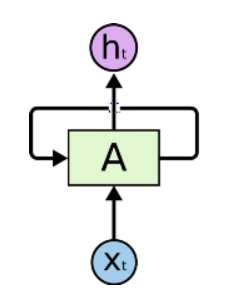
\includegraphics[width=0.17\textwidth]{recNeuNet} 
\caption{Rekurento neironu tīklu vienkārša reprezentācija} \cite{ANNTutorial} \label{rnnSimple} 
\end{figure}
   
    
RNN kļūdas var izplatīt vairāk nekā divos slāņos, lai iegūtu informāciju, kas ir bijusi daudz senāk. Šo procesu parasti sauc par izvēršanu. Diagrammā \ref{unfolding} varam apskatīt rekurentā neironu tīklu $A$ izvēršanu. Kā piemēru varam apskatīt situāciju, ja mūsu virkne ir 5 vārdu teikums. Šajā gadījumā tiks izveidots neironu tīkls ar 5 slāņiem, kur viens slāni saturēs informāciju par vienu vārdu.

 Diagrammā \ref{unfolding} $h_t$  ir slēpta stāvoklis laika solī $t$. Slēptajam slānim $h$ ir $M$ slēptās vienības $h_t = (h_1, h_2, ..., h_M)$, kas ir savstarpēji saistītas laikā ar rekurentiem savienojumiem. 
 
 Slēpto vienību inicializēšanai izmanto mazus nulles elementus, kas var uzlabot vispārējo veiktspēju un tīkla stabilitāti. Varam iedomāties slēpto stāvokli $h_t$ kā tīkla atmiņu. $h_t$ ir tas elements, kas saglabā informāciju par to, kas noticis visos iepriekšējos posmos, tāpēc to arī dēvē par tīkla $atmiņu$.
 
\begin{figure}[H] \centering
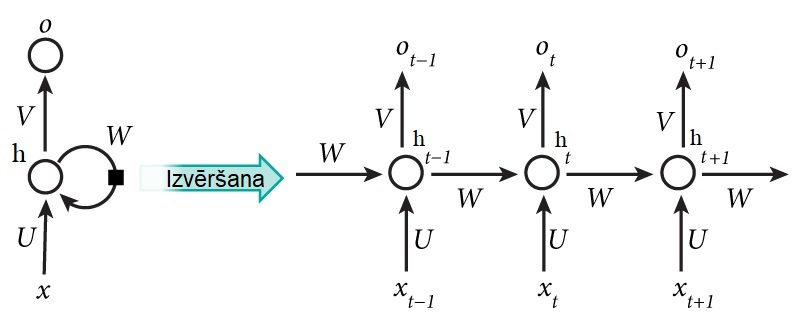
\includegraphics[width=0.70\textwidth]{rnnN} 
\caption{Rekurento neironu tīklu trīs laika posmu $izvēršana$} \cite{http://www.wildml.com/2015/09/recurrent-neural-networks-tutorial-part-1-introduction-to-rnns/} \label{unfolding} 
\end{figure}

    \begin{enumerate}
        
    \item Tīklam tiek padoti viena laika soļa ieejas dati jeb tīklam tiek padots ieejas datu mainīgais $x_t$ laika solī $t$. Piemēram, $x_1$ varētu būt vektors, kas atbilst teikuma otrajam vārdam.
    
    \item Tālāk aprēķina pašreizējo slēpto stāvokli, izmantojot pašreizējos ieejas datus un iepriekšējo stāvokli. Citiem vārdiem sakot, notiek $h_t$ aprēķins pēc formulas \ref{eq:hidden}.
    \begin{equation}
    h_t = f(U_{x_t}+W_{h_{t-1}})
    \label{eq:hidden}
    \end{equation}
     Funkcija $f$ parasti ir nelineāra, piemēram, tanh vai ReLU. $h_{t-1}$ kas ir nepieciešams, lai aprēķinātu pirmo slēpto stāvokli, parasti tiek inicializēts tā, ka visas sākuma vērtības ir nulles.
    
     $U,W,V$ ir parametru matricas. Atšķirībā no tradicionālajiem dziļajiem neironu tīkliem, kur katrā slānī tiek izmantoti dažādi parametri, RNN visos posmos izmanto vienādus parametrus $(U,W,V)$. Tas atspoguļo faktu par to, ka veic vienu un to pašu uzdevumu katrā posmā ar dažādiem ievades datiem. Tas ievērojami samazina kopējo parametru skaitu, ko nepieciešam iemācīties.

     
    \item Pašreizējais $h_t$ kļūst par $h_{t-1}$ nākamajā apstrādes posmā. Varam veikt nepieciešamos aprēķinus tik daudz laika posmiem, cik pieprasa konkrētā problēma. Pēc tam varam apvienot informāciju no visiem iepriekšējiem stāvokļiem.

    \item Kad visu laika posmu aprēķini ir pabeigti, pēdējo pašreizējo iegūto stāvokli izmanto, lai aprēķinātu izvades datus $o_t$. $o_t$  ir izejas dati laika solī $t$ un tie tiek aprēķināti, pamatojoties tikai uz atmiņu laikā $t$. Praksē tas ir nedaudz sarežģītāk, jo $h_t$ parasti nevar iegūt informāciju no soļiem, kas tikuši izpildīti pārāk sen atpakaļ.
    
      Ja apskata vienkāršu piemēru tad, ja grib paredzēt nākamo vārdu teikumā, tad izejas dati būtu visas dotās vārdnīcas varbūtību vektors \ref{softm}.
    \begin{equation}
    o_t = softmax(V_{h_t})
    \label{softm}
    \end{equation}
   
    Matemātiski $softmax$ funkcija paņem nenormalizētu vektoru un normalizē to, lai iegūtu varbūtības sadalījumu.

Diagrammā \ref{unfolding} ir parādīti izvades dati katrā laika posmā, bet atkarībā no uzdevuma, tas var arī būt nevajadzīgs. Piemēram, prognozējot teikumu mūs interesē tikai gala rezultāts, nevis katra individuāla vārda nozīme. Tāpat arī nav nepieciešamība pēc ievades datiem katrā laika posmā. RNN galvenā iezīme ir tieši slēptais stāvoklis, kurā tiek uztverta daļa informācijas no virknes \cite{http://www.wildml.com/2015/09/recurrent-neural-networks-tutorial-part-1-introduction-to-rnns/}.    
    
    \item Pēc tam izvades datus salīdzina ar patieso rezultātu, un pēc tam tiek aprēķināta kļūda izmantojot kļūdas funkciju.
    
   \item  Tad tiek pielietota atpakaļ izplatīšanās algoritms, lai atjaunotu svarus līdz brīdim, kad tīkls sasniedz kādu noteiktu mazu kļūdas slieksni vai izdara visas iterācijas un apstājas.    
    \end{enumerate}
     
	
 \subsection{Atpakaļ izplatīšanās laikā}

Uz priekšu izplatīšanās gadījumā ievaddati tiek padoti un pārvietojas uz priekšu katrā laika posmā. Bet gadījumā ar atpakaļ izplatīšanos figurāli iet atpakaļ laikā, lai mainītu svarus. Šo procesu sauc par atpakaļ izplatīšanos laikā.

Atpakaļ izplatīšanās algoritms rekurentajiem neironu tīkliem patiesībā ir līdzīgs parastajam neironu tīklam, tikai šai gadījumā apvienojam kļūdas gradientus visos laika posmos. 

Lai saprastu un vizualizētu atpakaļ izplatīšanos, nepieciešams apskatīt tīklu visos laika posmos. Jāatceras arī, ka RNN var vai nevar būt izejas dati katrā laika posmā un svari ir vienādi katrā laika posmā. 

Atpakaļ izplatīšanās laikā pamatprincips ir „izvēršana” \cite{bptt}. Visi rekurentie svari var tikt dublēti telpiski patvaļīgam laika posmu skaitam. Tas tiek apzīmēts, kā $\tau$. Līdz ar to katram mezglam, kas sūta aktivāciju tiešā vai netiešā veidā pa rekurentu savienojumu ir vismaz $\tau$ kopiju skaits, ko var redzēt attēlā \ref{bptt}. 

\begin{figure}[H] \centering
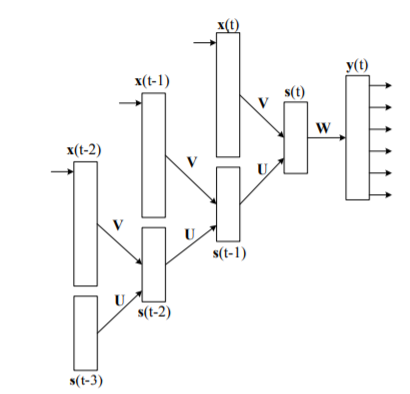
\includegraphics[width=0.45\textwidth]{bpttime} 
\caption{Tīkla izvēršanas($\tau = 3$)} \cite{bptt}  \label{bptt} 
\end{figure}

Kopējās kļūdas funkcija ir vienkārša standarta kļūdas funkcijas summa katrā laika posmā, ja tīkla apmācība sākas laika brīdi $t_0$ un beidzas laika brīdi $t_1$.

Vispirms tiek aprēķināta starpentropijas kļūda, izmantojot pašreizējos izvades datus un faktiskos izvades datus. RNN gadījumā, ja $y_t$ ir paredzamā vērtība un $\overline{y_t}$ ir faktiskā vērtība, kļūdu aprēķina kā savstarpēju entropijas zudumu \cite{bpttRNN}. To aprēķina konkrētā laika momentā $t$ izmantojot vienādojumus \ref{eq:entrophyLossInTimeStept} un kopējo izmantojot vienādojumu \ref{eq:totalEntrophyLoss}:
\begin{equation}
E_t(\overline{y_t}, y_t) = - \overline{y_t} log (y_t)
\label{eq:entrophyLossInTimeStept}
\end{equation}
\begin{equation}
E(\overline{y}, y) = - \sum \overline{y_t} log (y_t)
\label{eq:totalEntrophyLoss}
\end{equation}

Krītošā gradienta metode katrā laika solī veic svaru vērtību pārrēķinu  (atjaunošanu). Paredzētajam tīklam gradientu aprēķina katram laika posmam atkarībā no svara parametriem. 

Kad svari ir vienādi visos laika posmos, ņem gradientu no visiem laika posmiem un apvieno. Pēc tam svari tiek atjaunoti gan rekurentajiem neironiem, gan pilnībā savienotajiem slāņiem.

Kā piemēru varam apskatīt gadījumu, kad apstrādā pilnu virkni kā vienu apmācības piemēru, piemēram, ja nepieciešams izveidot vārdu. Šajā gadījumā kopējo kļūdu aprēķina, summējot kļūdu katrā laika posmā jeb kļūdu katrai rakstzīmei. 	
	
     \subsection{Ilgtermiņa atkarību problēma}
    Teorētiski RNN būtu jāvar saistīt iepriekšējo informāciju ar pašreizējo informāciju. Piemēram, izmantojot iepriekšējos vārdus, būtu jāvar saprast, kāds būs nākošais vārds. 
    
    Dažreiz ir nepieciešams tikai apskatīt jaunāko informāciju, lai veiktu nepieciešamo uzdevumu. Kā piemēru var apskatīt valodas modeli, kur vajag paredzēt nākamo vārdu, pamatojoties uz iepriekšējiem vārdiem. Ja cenšas prognozēt pēdējo vārdu teikumā \textit{"Mākoņi ir ..."}, nav nepieciešamības pēc papildu konteksta, lai zinātu, ka nākamais vārds visticamāk būs \textit{"debesīs"}. 
    
    Šādos gadījumos, ja starpība ir maza starp attiecīgajiem datiem un vietu, kur šie dati ir nepieciešami, tad ir iespējams apmācīt RNN izmantot iepriekšējo informāciju $X_0, X_1$, lai prognozētu pašreizējo informāciju $h_3$. Shematiski to var aplūkot attēlā \ref{RNNshorttermdepdencies}. 

\begin{figure}[H] \centering
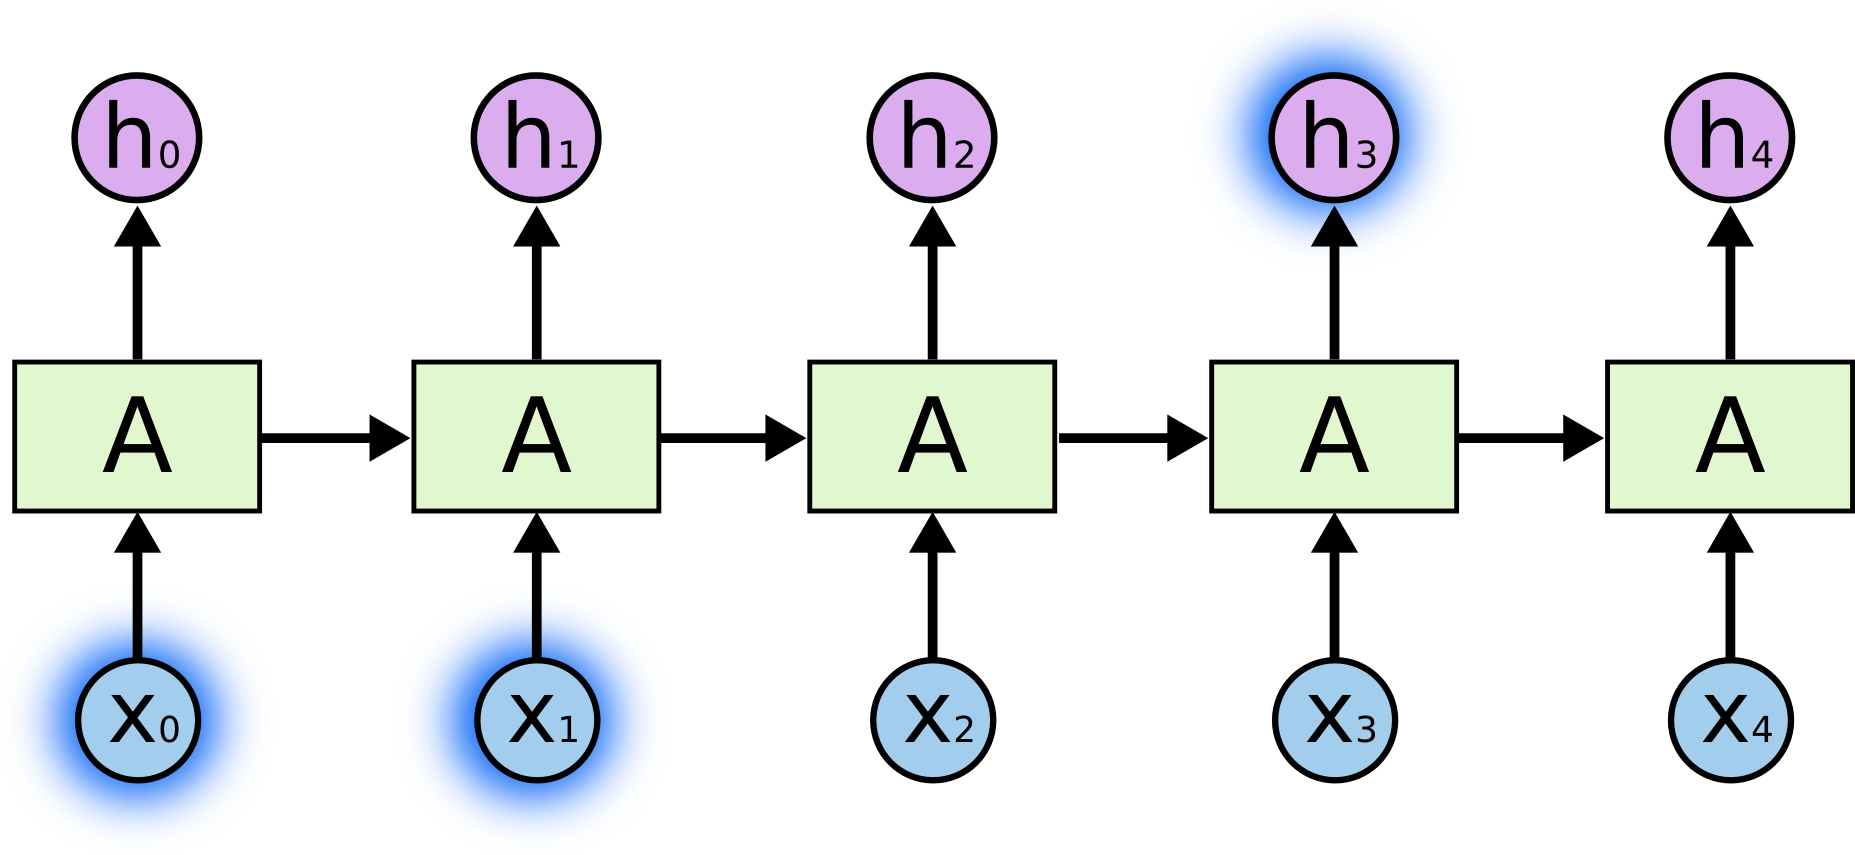
\includegraphics[width=0.50\textwidth]{RNNshorttermdepdencies} 
\caption{Atkārotot neirunu tīklu īstermiņa atkarība, kur $X_0,X_1, X_2, X_3 un X_4$ apzīmē ieejas datus konkrētā laika brīdī, $h_0,h_1, h_2, h_3, h_4$ izejas dati konkrētā laika brīdī un A reprezentē rekurento neironu tīklu.} 
\cite{ANNTutorial}
 \label{RNNshorttermdepdencies} 
\end{figure}

Bet ir arī gadījumi, kad nepieciešams vairāk konteksta. Piemēram ja vēlamies prognozēt pēdējo vārdu tekstā: \textit{"Es uzaugu Francijā ... es brīvi runāju ... valodā."} Visticamāk nākamajam vārdam, iespējams, ir jābūt valodas nosaukumam, bet ja vēlas sašaurināt valodas izvēli, ir nepieciešams zināt iepriekšējo kontekstu, par kuru tika runāts tālā pagātnē. 

Šādā gadījumā starpība starp attiecīgo informāciju un vietu, kur šī informācija ir nepieciešama, kļūst ļoti liela. Attēlā \ref{RNNlongtermdependencies} Jo vairāk šī atšķirība pieaug, jo grūtāk tīklam ir iespējams iemācīties savienot informāciju $X_0,X_1$, kas ir bijusi pagātnē, lai prognozētu pašreizējo informāciju $h_{t+1}$. 

\begin{figure}[H] \centering
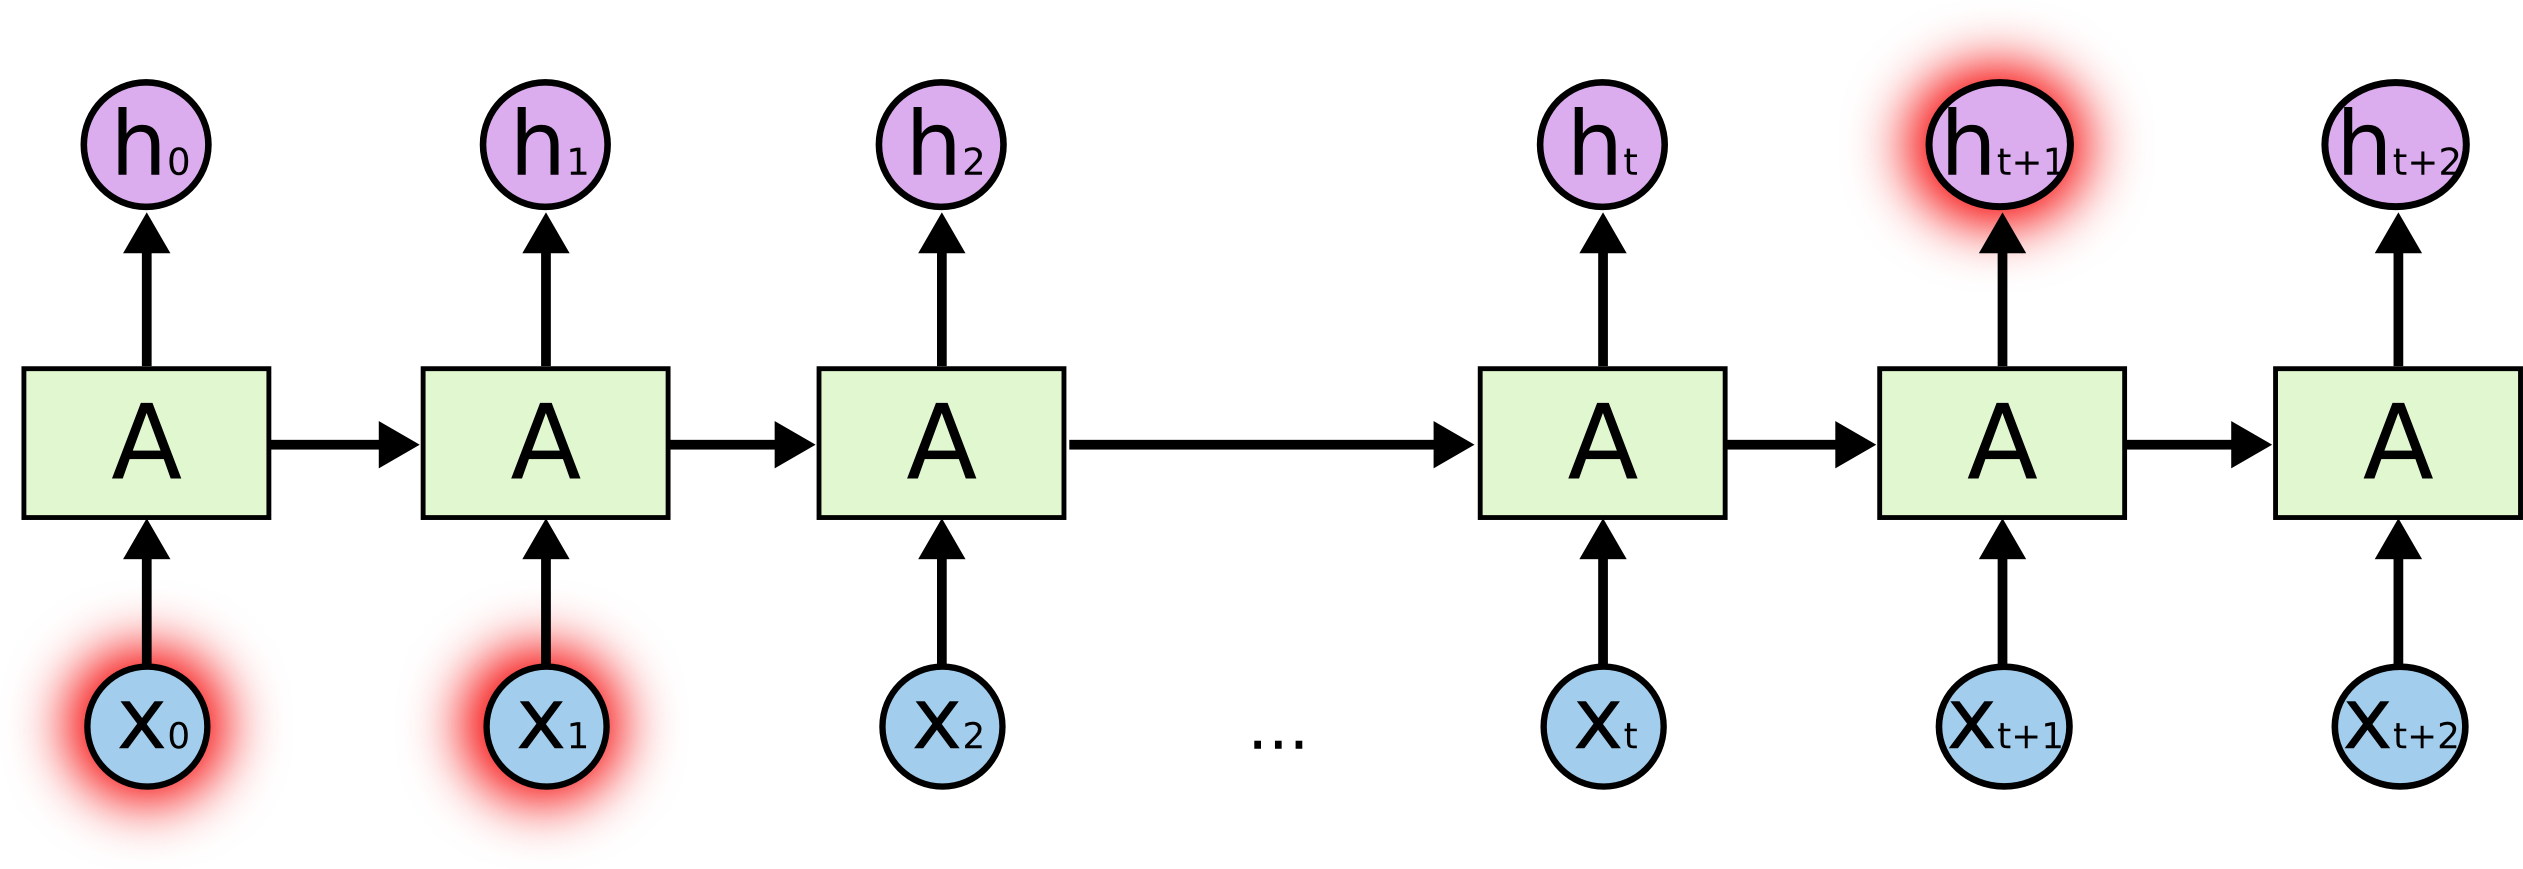
\includegraphics[width=0.70\textwidth]{RNNlongtermdependencies} 
\caption{Rekurento neironu tīklu ilgtermiņa atkarība, kur $X_t$ apzīmē ieejas datus konkrētā laika brīdī, $h_t$ izejas dati konkrētā laika brīdī un A reprezentē rekurento neironu tīklu.} 
\cite{ANNTutorial} \label{RNNlongtermdependencies} 
\end{figure}	
		
\section{ Ilgi-īslaicīgā atmiņa (Long Short-Term Memory)}
LSTM ir jauna rekurentā tīkla arhitektūra, kas izmanto atbilstošu uz gradienta balstītu mācību algoritmu. LSTM tīklam ievērojama ietekme ir bijusi valodu modelēšanā, runā-tekstā transkripcijā, mašīntulkojumā un citas lietojumprogrammās. 

LSTM ir līdzīga kontroles plūsma kā rekurentajam neironu tīklam. Tas apstrādā datus, kas pārsūta informāciju, kad tā tiek izplatīta uz priekšu. LSTM ir izstrādāts, lai pārvarētu kļūdas atpakaļ izplatīšanās problēmas, kas rodas RNN tīklā \cite{DBLP:journals/corr/abs-1808-03314}. 

Atšķirības ir darbībās, ko veic LSTM šūnas. LSTM paplašina RNN ar atmiņas šūnām, nevis periodiskām vienībām, lai saglabātu un izvadītu informāciju ilgā laika periodā, atvieglojot īstermiņa apmācības procesu. 

LSTM arī izmanto vārtus (no angļ. gates), kas ir mehānisms, kas balstīts uz komponenciālo ievades datu reizināšanu, kas nosaka katras atsevišķas atmiņas šūnas uzvedību. LSTM atjauno savu šūnu stāvokli, balstoties uz vārtu aktivizēšanas procesa. 

Ievades dati tiek padoti dažādiem vārtiem, kas kontrolē to, kādas darbības tiek veiktas šūnu atmiņā. Tas nozīme, ka šis tīkls var iemācīties savienot laika intervālus pat, ja tie pārsniedz 1000 soļus un ja rodas trokšņaini, nesavienojami ieejas dati \cite{rnnLstm}. Tas tiek panākts, izmantojot piemērotu gradienta algoritmu tīkla arhitektūrā, kas nodrošina vienmērīgu kļūdas plūsmu caur īpašu vienību iekšējo stāvokli. 

LSTM rekurentais slēptais slānis satur īpašas vienības, ko sauc par atmiņas blokiem. Atmiņas bloku var apskatīt attēlā \ref{lstm}. Atmiņas bloki satur atmiņu šūnas, kas satur pašsavienojumus, kas uzglabā īslaicīgu tīkla stāvokli, papildus īpašajām multiplikatīvām vienībām, ko sauc par vārtiem, kas nepieciešami, lai kontrolē informācijas plūsmu. 

\begin{figure}[H] \centering
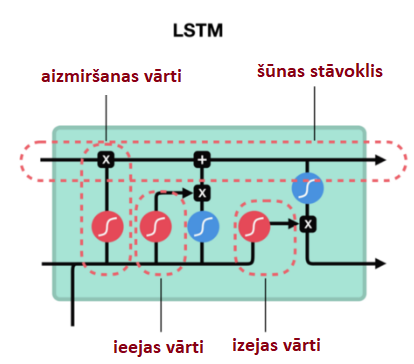
\includegraphics[width=0.40\textwidth]{lstmDeep} 
\caption{LSTM atmiņas bloka uzbūve} 
\cite{https://towardsdatascience.com/illustrated-guide-to-lstms-and-gru-s-a-step-by-step-explanation-44e9eb85bf21}
 \label{lstm} 
\end{figure}

Katrs atmiņas bloks oriģinālajā tīkla arhitektūras modelī satur ieejas vārtus un izejas vārtus. Ievades vārti kontrolē ieejas aktivizēšanas plūsmu atmiņas šūnā. Izvades vārti kontrolē šūnas izejas plūsmas aktivizēšanu pārējā tīklā. 

Vēlāk tīkla arhitektūrai tika mainīta un atmiņas blokam tika pievienoti aizmiršanas vārti. Tas tika izdarīts, lai samazinātu LSTM modeļa problēmu, kas neļauj tiem veikt nepārtrauktu ievades datu plūsmas apstrādi, ja dati nav segmentēti pa apakškopām.

Turklāt mūsdienu LSTM arhitektūrā ir pievienots ķēdes savienojums no iekšējām šūnām uz vārtiem, kas atrodas tai pašā šūnā, lai būtu iespējams noteikt precīzu izejas laiku \cite{ANNTutorial}.

Bet tomēr izmantojot LSTM jārēķinās ar to, ka šis tīkls cieš no augstas sarežģītības slēptajos slāņos. Tipiskam LSTM ir aptuveni četras reizes vairāk parametru nekā vienkāršam RNN. Kaut arī LSTM ir parādījis uzlabotas spējas iemācīties ilgtermiņa laika atkarības, tomēr tiek apgalvots, ka tīkla aizture mehānismiem nav iespējas visaptveroši diskriminēt būtiskāko un nesvarīgāko informāciju \cite{salehinejad2017recent}. Tāpēc LSTM grūti ir uzdevumi, kā darbības atzīšana, kur sekvences bieži var saturēt daudzus nesvarīgus kadrus.



\subsection{Arhitektūra}
\subsubsection{Aizmiršanas vārti}

Pirmkārt, ir aizmiršanas vārti. Šie vārti izlemj, kāda informācija ir jāizmet un ko nepieciešams saglabāt. Informācija no iepriekšējā slēpta stāvokļa un informācija no pašreizējās ievades tiek nodota caur sigmoidas funkciju. 

Tiek atgrieztas vērtības no $0$ līdz $1$. Jo tuvāk $0$ vērtībai nozīmē, ka informāciju var aizmirst, un jo tuvāk $1$ nozīmē, ka informāciju jāsaglabā. Aizmiršanas vārti mēra šūnas iekšējo stāvokli pirms pievienot to tā kā ieejas datus šūnai, izmantojot šūnas pašregulācijas savienojumu, tādējādi adaptīvi aizmirstot vai atiestatot šūnas atmiņu \cite{https://towardsdatascience.com/illustrated-guide-to-lstms-and-gru-s-a-step-by-step-explanation-44e9eb85bf21}.


\subsubsection{Ieejas vārti}


Lai atjauninātu šūnas stāvokli, ir ieejas vārti. Pirmkārt, tiek nodots iepriekšējais slēptais stāvoklis un pašreizējā ievade sigmoidas funkcijai. Tas izlemj, kuras vērtības tiks atjauninātas, pārveidojot vērtības no 0 līdz 1. 0 nozīmē, ka tās nav svarīgas, un 1 ir svarīgas. Arī tiek nodots slēptais stāvoklis un pašreizējā ievade $tanh$ funkcijai, lai saspiestu vērtības starp -1 un 1, tas palīdz regulēt tīklu. Tad sareizina $tanh$ izvades datus ar sigmoidas izvades datiem. Sigmoidas funkcija izlems, kura informācija ir svarīga no $tanh$ funkcijas atgrieztās informācijas. Šīs funkcijas var redzēt attēlā \ref{lstmActivation}.

\begin{figure}[H] \centering
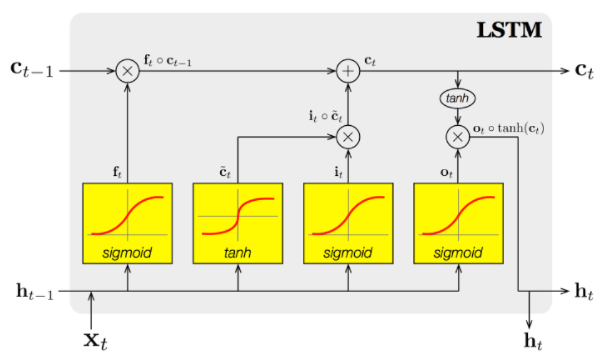
\includegraphics[width=0.60\textwidth]{lstmActivation} 
\caption{LSTM Atmiņas šūnas elementi}
\cite{https://medium.com/@kangeugine/long-short-term-memory-lstm-concept-cb3283934359}
  \label{lstmActivation} 
\end{figure}


\subsubsection{Šūnu stāvoklis}

Tagad vajadzētu būt pietiekamai informācijai, lai aprēķinātu jauno šūnas stāvokli. Pirmkārt, šūnas stāvoklis tiek reizināts ar aizmiršanas vektoru. Šai gadījuma ir iespēja izmest konkrētas vērtības šūnas stāvoklī, ja šūnas stāvokli reizināta ar vērtībām, kas ir tuvu pie 0. Pēc tam ņem izejas datus no ievades vārtiem un veic saskaitīšanu, šādā veidā atjauno šūnas stāvokli ar jaunām vērtībām, kuras neironu tīkls uzskata par atbilstošām. Beigās tiek iegūts jauns šūnu stāvoklis.

\subsubsection{Izejas vārti}

Pēdējais posms ir izvades vārti. Izvades vārti nosaka, kādam jābūt nākamajam slēptajam stāvoklim. Slēptais stāvoklis satur informāciju par iepriekšējiem ievades datiem. Slēpto stāvokli izmanto arī prognozēm. 

Pirmkārt, iepriekšējo slēpto stāvokli un pašreizējos ievades datus padod sigmoidas funkcijai. Tad nodod jauni veidoto šūnu stāvokli $tanh$ funkcijai. Reizina $tanh$ funkcijas izvades datus ar sigmoidas izvades datiem, lai izlemtu, kādai informācijai jābūt slēptā stāvoklī. Šīs funkcijas var redzēt attēlā \ref{lstmActivation}. Un no tā veidojas jaunie izvades dati, kas ir slēptais stāvoklis. Jaunais šūnu stāvoklis un jaunais slēptais stāvoklis tiek pārnests uz nākamo laika soli. 

\subsubsection{Ķēdes savienojumi}
Viena LSTM variācija ir tāda, ka šūnai tiek pievienoti ķēdes savienojumi. Tas nozīmē, ka vārti var aplūkot šūnu stāvokli. Bieži vien tiek veidoti ķēdes savienojumi, kas ļauj vārtiem būt atkarīgiem ne tikai no iepriekšējā slēptā stāvokļa st − 1, bet arī no iepriekšējā iekšējā stāvokļa ct − 1.  Ķēdes savienojumi palīdz iemācīties precīzus notikumu laikus. LSTM, ko papildina ar ķēdes savienojumiem spēj no iekšējām šūnām līdz multiplikatīvajiem vārtiem iemācīties smalka atšķirība starp pīķu secībām, kas izvietotas piemēram 50 vai 49 laika posmos attālumā.

\subsubsection{Savienotie aizmiršanas un ievades vārti}
Vēl viena variācija ir savienot aizmiršanas un ievades vārtus.  Tā vietā, lai atsevišķi nolemtu, ko aizmirst un kādu jaunu informāciju vajadzētu pievienot, šis lēmums tiek pieņemts kopā. Tātad sūnā aizmirst tikai tad kad ir informācija ar kuru var aizvietot iepriekšējo informāciju un pretēji. %https://www.csie.ntu.edu.tw/~yvchen/f105-adl/doc/161124_GatingMechanism.pdf

\subsubsection{Slēgtās Rekurentās Vienības}
Slēgtās Rekurentās Vienības (angļ. val. Gated Recurrent Unit) vai GRU ir LSTM variācija. Šajā modelī tiek apvienots šūnu stāvoklis un slēptais stāvoklis un notiek vēl citas izmaiņas. Atšķirībā no LSTM, GRU ir vienkāršāka arhitektūra un prasa mazāk aprēķinu. Vairāk var par šo tīklu var uzzināt \cite{ANNTutorial}.


\subsection{Šūnas un slēptā stāvokļa atjaunošana}
 
\begin{figure}[H] \centering
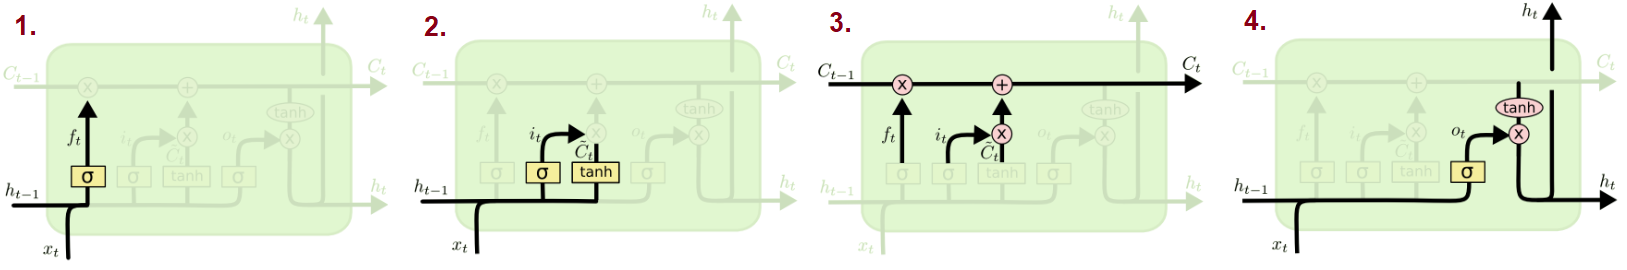
\includegraphics[width=1.01\textwidth]{lstmSteps} 
\caption{Tīkla vienības aktivizēšanās shēma}
\cite{ANNTutorial}
  \label{lstmDeep} 
\end{figure}

LSTM tīkls izveido ieejas sekvences kartēšanas secību \cite{sak2014long}, kuru var apskatīt attēlā \ref{lstmDeep}, no $x = (x_1, ..., x_T)$ līdz izejas virknei $y = (y_1, ..., y_T)$. To dara tā, ka  aprēķina tīkla vienības aktivizēšanos.
  
 Lai aprēķinātu tīkla vienības aktivizāciju, atmiņas bloka elementiem tiek izmantoti dažādi vienādojumi, darbības tiek veiktas iteratīvi no $t = 1$ līdz $T$. 
 
Aizmiršanas vārtu vienādojumu apraksta ar formulu \ref{eq:Aizmiršanas vārtu vienādojums}.
Ievades vārtu vienādojumu apraksta ar formulu \ref{eq:Ievades vārtu vienādojums}.
Ieejas modulācijas vārtu vienādojumu apraksta ar formulu \ref{eq:Ieejas modulācijas vārtu vienādojums}.
Šūnas stāvokļa vienādojumu apraksta ar formulu \ref{eq:Šūnas stāvokļa vienādojums}.
Izvades vārtu vienādojumu apraksta ar formulu \ref{eq:Izvades vārtu vienādojums}.
Slēptā stāvokļa vienādojumu apraksta ar formulu \ref{eq:Slēptā stāvokļa vienādojums}.
Izvades datu vienādojumu apraksta ar formulu \ref{eq:Izvades datu}.

\begin{equation}
f_t = \sigma (W_{fx}x_t + W_{fh}h_{t-1} + W_{fc}c_{t-1} + b_f)\label{eq:Aizmiršanas vārtu vienādojums}
\end{equation}

\begin{equation}
i_t = \sigma (W_{ix}x_t + W_{ih}h_{t-1} + W_{ic}c_{t-1} + b_i)
\label{eq:Ievades vārtu vienādojums}
\end{equation}

\begin{equation}
\overline{c} = g (W_{cx}x_t + W_{ch}h_{t-1} + b_c) \label{eq:Ieejas modulācijas vārtu vienādojums}
\end{equation}

\begin{equation} c_t = f_t \odot c_{t-1} + i_t \odot \overline{c}
\label{eq:Šūnas stāvokļa vienādojums}
\end{equation}

\begin{equation} o_t = \sigma (W_{ox}x_t + W_{oh}h_{t-1} + W_{oc}c_t + b_o) \label{eq:Izvades vārtu vienādojums}
\end{equation}

\begin{equation} h_t = o_t \odot m(c_t)
\label{eq:Slēptā stāvokļa vienādojums}
\end{equation}

\begin{equation}
y_t = \phi(W_{yt}ht+b_y)
\label{eq:Izvades datu}
\end{equation}


$W$ termini apzīmē svara matricas (piemēram, $W_{ix}$ ir svaru matrica no ieejas vārtiem līdz ievadam),$W_{ic}, W_{fc}, W_{oc}$ ir diagonālās svara matricas ķēdes savienojumiem. $b$ termini apzīmē nobīdes (angļ. bias)vektorus ($b_i$ ir ieejas vārtu nobīdes vektors). $\sigma$ ir loģistikas sigmoidas funkcija. $i, f, o$ un $c$ ir attiecīgi ievades vārti, aizmiršanas vārti, izejas vārti un šūnu aktivācijas vektori, visi šie lielumi ir tādi paši kā šūnas izvades aktivizēšana vektors $h$, $h$ šūnas aktivizēšana vektors.
$c_{t-1}$ iepriekšējā šūnas aktivizācijas vektors, $\odot$ ir vektoru elementi, $g$ un $m$ ir šūnas ievades un šūnu izvades aktivizācijas funkcijas, parasti $tanh$.
$\phi$ ir tīkla izvades datu aktivizācijas funkcija piemēram, $softmax$. 

\begin{enumerate}
\item Vispirms tiek apvienots iepriekšējais slēptais stāvoklis un pašreizējā ievade. Šo procesu sauc par apvienošanu. Apvienotie dati tiek padoti aizmiršanas vārtiem. Šajā slānī tiek izdalīti dati, kuri netiks izmantoti tālāk. Tiek apskatīts $h_{t-1}$ un $x_t$, un katram $c_{t-1}$ elementam tiem izdots skaitli no 0 līdz 1, lai noteiktu ko aizmirst. Kā vizuāli, tas ir attēlots var redzēt attēla \ref{lstmDeep} pirmajā solī. 

\item Kandidāta slānis tiek izveidots, izmantojot apvienošanas datus. Kandidāts satur iespējamās vērtības, kuras var pievienot šūnas stāvoklim. Tālāk apvienotie dati arī tiek padoti ievades slānim. Šis slānis nosaka, kādus kandidāta datus vajadzētu pievienot jaunajam šūnu stāvoklim. Vispirms sigmoids slānis, ko sauc par ieejas vārtu slāni, nolemj, kuras vērtības tik atjauninātas. Tālāk $tanh$ slānis rada jaunu kandidātu vērtību vektoru $\overline{c_t}$, kas varētu būt pievienots stāvoklim. Trešajā posmā apvieno kandidātu vektoru un ieejas vārtu slāni, lai izveidotu stāvokļa atjauninājumu. Kā vizuāli, tas ir attēlots var redzēt attēla \ref{lstmDeep} otrajā solī.
%https://cedar.buffalo.edu/~srihari/CSE676/10.10%20LSTM.pdf

\item Pēc aizmiršanas slāņa, kandidāta slāņa un ievades slāņa aprēķināšanas tiek aprēķināts šūnas stāvoklis. Tiek izmantoti visi šie vektori un iepriekšējais šūnas stāvoklis. Tiek reizināts vecais stāvoklis ar $f_t$, aizmirstot informāciju, kuru nolēma aizmirst agrākajā fāzē. Tad pievieno $ i_t \odot \overline{c_t}$. Tās ir jaunās kandidāt vērtības, kas ir mērogotas atkarībā no tā cik daudz ir nolemts atjaunināt katru šūnas stāvokļa vērtību. Kā vizuāli, tas ir attēlots var redzēt attēla \ref{lstmDeep} trešajā solī.

\item Tiek aprēķināti izejas dati. Vispirms izmanto sigmoidu slāni, kas izlemj, kādas šūnu stāvokļa daļas tiks izvadītas. Šūnu stāvoklis iet caur $tanh$, lai mērogotu vērtības no -1 līdz 1. Pēc tam šie dati tiek reizināti ar sigmoid vārtu izejas datiem, lai tiktu izvadīta tikai informācija, kuru nolēmām atcerēties iepriekš. Sareizinot izejas datus un jauno šūnu stāvoklis tiek iegūts jaunais slēptais stāvoklis. Kā vizuāli, tas ir attēlots var redzēt attēla \ref{lstmDeep} ceturtajā solī.

\end{enumerate}


\section{Apvienotā arhitektūra (CNN + LSTM)}
%https://www.sciencedirect.com/science/article/pii/S1566253518300460
CNN - LSTM arhitektūra atšķiras no tradicionāli tīras CNN vai tīras LSTM arhitektūras. Pirmā puse ir CNN, un tā tiek izmantota īpašību iegūšanai. Pēdējā daļa ir LSTM, kas veic prognozēšanu, izmantojot īpašības, ko ieguva CNN, lai analizētu un novērtētu kādi būs izejas dati nākamajā laika posmā.

Turklāt eksperimenti liecina, ka LSTM un CNN iemācās dažādas īpašības, kad tiek apmācīti pie tiem pašiem datiem. Šī atšķirība rada iespēju apvienot īpašības, kuras iemācījušies gan 
CNN un LSTM, vienā modelī. Tas dod iespēju iegūt labāku precizitāti nekā tad, kad tiek izmantos katrs modelis patstāvīgi \cite{geras2015blending}. 

 CNN - LSTM parasti tiek izmantots, ja ievades datiem ir telpiska struktūra, piemēram, 2D struktūra vai pikseļi attēlā \ref{cnnLstm} vai arī 1D vārdu struktūra teikumā, rindkopā vai dokumentā. Kā arī ievades dati satur laika struktūra, piemēram, secīgi attēli, kas veido video, vai vārdi tekstā vai arī, ja nepieciešams ģenerēt izejas datus, kam piemīt laika struktūra, piemēram, aprakstošus teikumus \cite{lstmCNNTut}. 
 
 Tātad CNN - LSTM arhitektūra ietver CNN slāņu izmantošanu, lai veiktu ievades datu aprakstošo īpašību izgūšanu un apvienojot ar LSTM tīkls var veikt virknes datu prognozēšanu.
 
 \begin{figure}[H] \centering
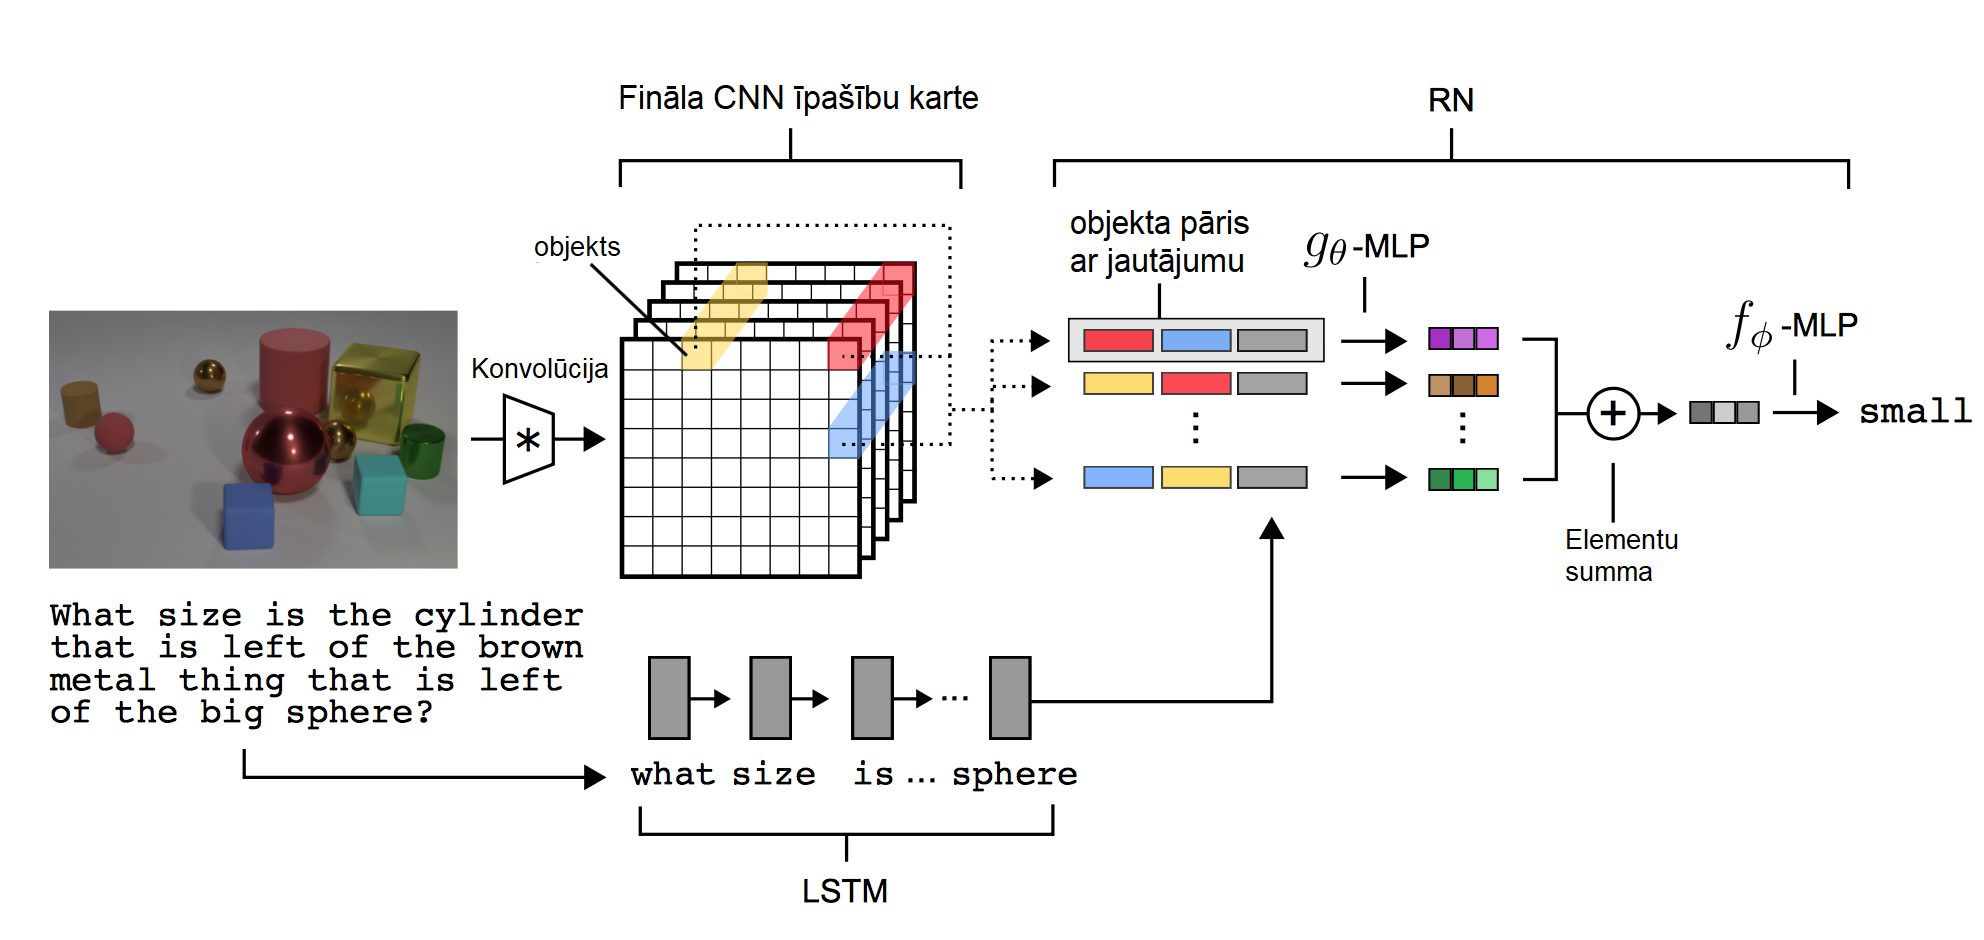
\includegraphics[width=0.80\textwidth]{cnnLstm} 
\caption{Modelim ir jāaplūko dažādu formu, izmēru, krāsu objekti un jāspēj atbildēt uz jautājumiem, kas saistīti ar vairākiem šādiem objektiem.} \cite{https://hackernoon.com/deepmind-relational-networks-demystified-b593e408b643}  \label{cnnLstm} 
\end{figure}

 CNN un LSTM kombinācija vienotā sistēmā jau ir piedāvājusi jaunākos rezultātus runas atpazīšanas domēnā, kur nepieciešama modelēšana, kas prasa laiku informāciju \cite{article}. Šāda veida arhitektūra spēj uztvert laika atkarību no īpašībām, kas iegūtās izmantojot konvolūcijas operāciju. 
 
Kā piemēru varam apskatīt $DeepConvLSTM$ struktūras arhitektūru  \ref{deepCnnLstm}, kas tik izmantota avotā \cite{https://www.mdpi.com/1424-8220/16/1/115}, lai atpazītu aktivitātes.

\begin{figure}[H] \centering
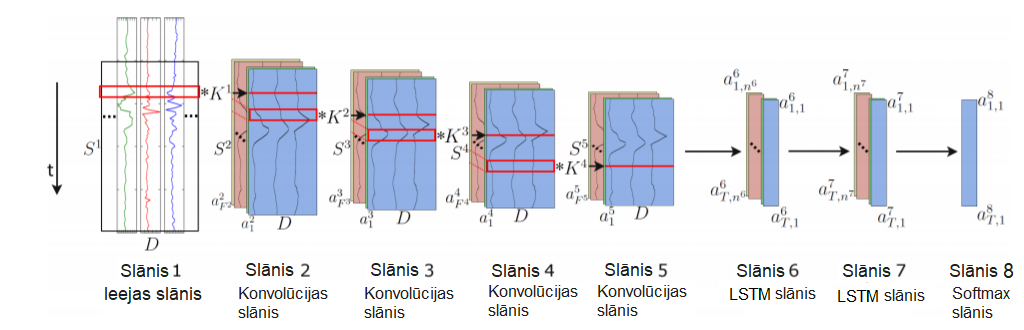
\includegraphics[width=0.90\textwidth]{sigDeepLSTm} \caption{DeepConvLSTM arhitektūru} \cite{https://www.mdpi.com/1424-8220/16/1/115}  \label{deepCnnLstm} 
\end{figure}


 Attēlā \ref{deepCnnLstm} no kreisās puses signāli, kas nāk no valkājamajiem sensoriem, tiek apstrādāti ar četriem konvolūcijas slāņiem, kas ļauj mācīties no datiem. Pēc tam divi pilnībā savienotie slāņi veic nelineāru transformāciju, kas dod klasifikācijas rezultātu izejas slānī pa labi ar $softmax$ loģistisko regresiju. 

1. slāņa ievade dati  atbilst sensora datiem, kuru izmērs ir $D x S^1$. $D$ apzīmē numuru sensoru kanālu un $S^l$ īpašības karšu garuma konkrētā slānī $l$. 

2. – 5. Slāņi ir konvolūcijas slāņi. $K^l$ apzīmē kodolus konkrētā $l$ slānī (attēloti kā sarkani kvadrāti). $F^l$ apzīmē īpašību karšu skaitu konkrētā $l$ slānī. Konvolūcijas slāņos $a^l_i$ apzīmē aktivāciju, kas nosaka īpašību karti $i$ slānī $l$.
 
  6. un 7. slānis ir LSTM slāņi. LSTM slāņos: $a^l_{t,i}$ apzīmē vienības $i$ aktivizēšanu slēptajā slānī $l$ laikā posmā $t$. Laika ass ir vertikāla. 

Šajā modelī netiek lietoti apvienošanas slāņi, jo tiek uzskatīts, ka apvienošanas slāņu izmantošana pēc konvolūcijas slāņiem traucē konvolūcijas slāņu spējai iemācīties samazināt neapstrādāta sensora datus. 
 
Apkopojumā modelim ieejas dati tiek padoti CNN slānim, kur notiek datu transformācijas, kas aprakstītas iepriekš nodaļā par Konvolūcijas neironu tīkliem, un galā tiek iegūta ieejas datu reprezentācija īpašību telpā. Pēc tam pēdējā CNN slāņa iegūtās īpašības tiek izmantotas LSTM slāņos, lai iegūtu secīgu laika informāciju. Pēdējā LSTM slāņa pēdējo slēpto vektoru izmanto $softmax$ klasifikators, lai ģenerētu klašu etiķetes, kas tiek salīdzināta ar patieso klašu etiķeti, tādā veidā nosakot tīkla precizitāti. 


\section{Izzūdošais un eksplodējošais gradients}

Stohastiskais krītošais gradients (angļ. stochastic gradient descent) šķiet pietiekami vienkāršs process, bet daudzos tīklos var pamanīt, ka svari, kas ir tuvāk tīkla beigām, mainās daudz vairāk nekā sākumā \cite{bengio1994learning}. Un jo dziļāks tīkls, jo mazāk un mazāk sākuma slāņi mainās. 

Problēma rodas, jo svari tiek inicializēts nejauši. Ja tie gandrīz vai nemainās, tad tie nekad nespēs sasniegt pareizās vērtības vai arī apmācība aizņems gadus.

RNN apmācības laikā aprēķina izeju datus ar vēlamajiem izejas datiem. Un apmācības laikā kļūdas funkcija salīdzina iegūtos rezultātus, kas attēlā \ref{VanishingGradient} ir attēloti ar sarkaniem apļiem, ar vēlamo rezultātu. Beigās iegūst šīs vērtības visā laika rindā, katram atsevišķam sarkanajam aplim. 

Pēc tam kļūdas funkcijas (no angļ. cost function) vērtība tiek atpakaļ izplatītas tīklā atkarībā no tā, cik daudz laika soļi tikuši veikti, to var redzēt pa labi attēlā \ref{VanishingGradient}.

\begin{figure}[H] \centering
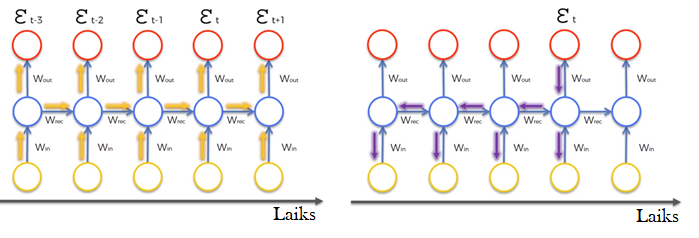
\includegraphics[width=0.80\textwidth]{VanishingGradient} 
\caption{Gradienta aprēķināšana gaita. Pa kreisi parādīts, kā tiek aprēķināta kļūda katrā laika posmā un pa labu tiek parādīts, kā notiek kļūdas atpakaļ izplatīšana} \cite{https://www.superdatascience.com/recurrent-neural-networks-rnn-the-vanishing-gradient-problem/}
 \label{VanishingGradient} 
\end{figure}


Kā piemēru, varam apskatīt vienu kļūdas posmu $e_t$ kādā laika brīdī $t$.

Pirmkārt, tiek aprēķināta kļūdas funkcija (cost function) $e_t$, un pēc tam nepieciešams izplatīt kļūdas funkciju atpakaļ visā tīklā, jo ir nepieciešams atjaunināt svarus. Būtībā ikvienam neironam, kas piedalījās izejas datu aprēķināšanā un ir saistīts ar kļūdas funkciju, nepieciešams veikt svaru atjaunošanu, lai mazinātu kļūdu.
 
Izmantojot RNN ir jāatceras, ka ne tikai neironiem, kas darbojas tieši zem konkrētā izvades slāņa, bet visiem neironi, kas atrodas tālu atpakaļ laikā, nepieciešams atjaunot svarus. Tas nozīme, ka ir nepieciešams doties atpakaļ laikā līdz šiem neironiem. 

Problēma ir tieši saistīta ar $W_{rec}$ atjaunināšanu. $W_{rec}$ ir svari, kas tiek izmantoti, lai savienotu slēptos slāņus pašus ar sevi izkliedētā laika cilpā un tos sauc par rekurentajiem svariem. Piemēram, lai nokļūtu no $x_{t-3}$ līdz $x_{t-2}$ ir  jāreizina $x_{t-3}$ ar $W_{rec}$. Tad, lai nokļūtu no $x_{t-2}$ uz $x_{t-1}$, atkal notiek reizināšana $x_{t-2}$ ar $W_{rec}$. 

Tātad, rezultātā reizina ar vieniem un tiem pašiem svariem vairākas reizes, un tieši šeit rodas problēma. Ja reizina kaut ko ar mazu skaitli iegūstam to, ka vērtība samazinās ļoti ātri. 

Svari sākumā tiek izinicializēti ar gadījuma vērtībām, kas ir tuvu nullei, un no turienes tīkls sāk pielāgot svarus apmācības procesā. Bet, ja sākt ar $W_{rec}$, kura vērtības ir tuvu nullei un pēc tam reizināt $x_t, x_{t-1}, x_{t-2}, x_{t-3}, ...$ ar šīm vērtībām, gradients ar katru reizinājumu kļūst arvien mazāks un mazāks. Un jo mazāks ir gradients, jo grūtāk tīklā atjaunināt svarus un ilgāk, lai sasniegtu gala rezultātu \cite{https://www.superdatascience.com/recurrent-neural-networks-rnn-the-vanishing-gradient-problem/}. 

Apkopojumā, ja $W_{rec}$ ir mazs, tad ir izzūdošā gradienta problēma, un, ja $W_{rec}$ ir liels, rodas eksplodējošā gradienta problēma  \ref{exploadingGradient}. Izzūdošā gradienta problēmas gadījumā, jo tālāk ejam cauri tīklam, jo zemāks ir gradients, un tas noved pie tā, ka kļūst grūtāk apmācīt svarus. Tas ir kā domino efektu, kas ietekmē visus turpmākos svarus visā tīklā.


\begin{figure}[H] \centering
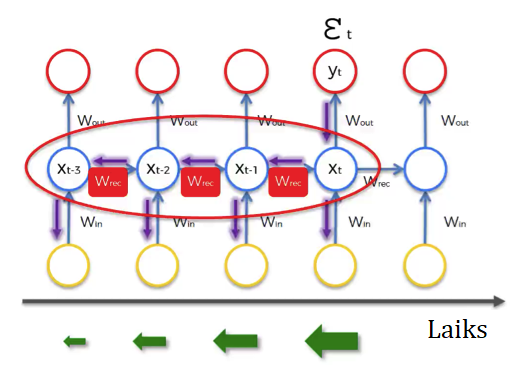
\includegraphics[width=0.50\textwidth]{GradientIssue} 
\caption{Gradienta izzušanas un eksplodēšanas problēmas attēlojums}
\cite{https://www.superdatascience.com/recurrent-neural-networks-rnn-the-vanishing-gradient-problem}
  \label{exploadingGradient} 
\end{figure}

%\begin{equation}
%\Pi{t\geq i>k}W^T_{rec}diag(\sigma'(x_{i-1}))
%$\label{https://github.com/Achronus/Machine-Learning-101/wiki/Recurrent-Neural-Networks-(RNN)}
%\end{equation}

\subsubsection{Eksplodējošā gradienta gadījumā varam:}
\begin{itemize}
\item Pārtraukt atpakaļ izplatīšanu pēc noteikta punkta, bet tas parasti nav optimāls, jo ne visi svari tiek atjaunināti;
\item Sodīt vai mākslīgi samazināt gradientu;
\item Noteikt maksimālo gradientu robežu.
\end{itemize}

\subsubsection{Izzūdošā gradienta gadījumā varam:}
\begin{itemize}
\item Inicializēt svarus tā, lai samazinātu izzušanas gradienta potenciālu;
\item Izmantot Atbalsta stāvokļa tīklus (angļ. Echo State Networks), kas paredzēti izzūdošā gradienta problēmas risināšanai;
\item Izmantot Ilgi-īslaicīgos atmiņas tīklus (angļ. Long Short-Term Memory 
Networks).
\end{itemize}

 
%\chapter{Programmatūras ietvari}
%Autors pētījuma laikā, darba izstrādei izvēlējās Python programmēšanas valodā piedāvātos risinājumus. Pieejamās Python bibliotēkas ir ērtas un viegli izmantojamas, lai izveidotu tīkla arhitektūras, kas tiks izmantotas darbā. Kā arī lai veiktu izveidoto tīklu pamācību un testēšanu. Python piedāvātie risinājumi arī tiek izmantoti, lai veiktu datu kopas sagatavošana. Lai iegūtu datu kopu nepieciešama datu ielasīšana un izgūšana no failiem ar Eiropas datu formātu.

%\section{TensorFlow}

%TensorFlow ir atvērtā koda programmatūras bibliotēka \cite{tensorflow2015-whitepaper}. Elastīgā arhitektūra ļauj ērti veikt aprēķinus izmantojot dažādas platformas - CPU, GPU. Tensorflow bieži izmanto mašīnmācīšanās un dziļās apmācības procesā. TensorFlow piedāvā dažādus rīkus, kas ļauj veidot modeļus pēc vēlamā abstrakcijas līmeņa. To var  izmantot, lai norādītu iepriekš noteiktas arhitektūras, piemēram, lineāro regresiju vai neironu tīklus. 

%Bet tomēr Tensorflow ir arī mīnusi. Piemēram, skaitļošanas ātrumam TF atpaliek, tiek vairāk veikta koncertēšanas uz ražošanas vidi, nevis uz veiktspēju. Kā arī nav GPU atbalsta un vienīgais pilnais valodas atbalsts ir Python.

%\section{Keras}

%Keras ir atvērta avota neironu tīkla bibliotēka, kas rakstīta Python. 
%Tas spēj darboties virs TensorFlow, Microsoft Cognitive Toolkit vai Theano. Paredzēts ātrai eksperimentēšanai ar dziļajiem neironu tīkliem. Keras koncentrējas uz to, lai šī bibliotēka būtu  lietotājam draudzīga, modulāra un paplašināma \cite{chollet2015keras}.

%Bet neskatoties uz to Keram tomēr ir trūkumi. Keras neironu tīklu izveido padara diezgan vienkāršu, bet tomēr dažreiz ir vajadzīga lielāka kontrole pār algoritma detaļām. Keras ir mazāk elastīgas šajā gadījumā nekā citas bibliotēkas. Kā arī slikti atbalsta paralēlo un GPU skaitļošanu. 

%\section{Visbrain}

%Visbrain ir atvērtā koda Python 3 pakete, kas paredzēta smadzeņu signālu vizualizācijai. No šīs paketes tiks izmantots “Sleep”. Tas ir elastīgs grafiskais lietotāja interfeiss, lai vizualizētu, analizētu un novērtētu polisomnogrāfisko miega datus. 

%Šis interfeiss iever sevī polisomnogrāfisko datu, spektrogrammas, hipnogrammu un topogrāfisko karšu dinamisku parādīšana ar vairākiem pielāgojamiem parametriem. 

%Programmatūras pakotne atbalsta ne tikai plašu komerciālo datu formātu, bet arī standarta failu formātu, piemēram, Eiropas datu formātu ielasīšanu un datu izgūšanu. “Sleep” tiek veidots uz VisPy bibliotēkas, kas nodrošina ātrdarbīgu un augsta līmeņa vizualizāciju. \cite{10.3389/fninf.2017.00060} 

\chapter{Prakstiskā daļa}


\section{Datu sagatavošana}
\subsubsection{Datu kopa}
%Datubāze tiek ņemta no https://physionet.org/physiobank/database/sleep-edfx/sleep-cassette/
Tika apskatītas dažādas miega EEG datu bāzes. Un tika izlemts lietot datubāzi \cite{goldberger2000physiobank}, lai veiktu tīklu apmācību un testēšanu. Šī datubāze satur 61 polisomnogrammu kolekciju ar pavadošām hipnogrammām. Šajā datu kopā visi EDF galvenes lauki atbilst arī EDF + specifikācijām, kas ļauj izmantojot Visbrain pieejamo funkcionalitāti, lai nolasītu hipnogrammas datus. Hipnogrammā \ref{hypnoGramS} uz y ass tiek attēlota informācija par miega fāzēm un uz x ass tiek attēlots laiks, kuru cilvēks pavada miegā. Šajā gadījumā visas nakts ieraksta laiks tiek apzīmēts sekundēs, sākot ar 0:00 līdz 0:47. Datubāzes EDF faili ir pilnas nakts polisnogrāfiski miega ieraksti, kas satur EEG, EOG (Elektrookulogrāfija),deguna gaisa plūsmu, taisnās zarnas temperatūru, submentālo EMG (Elektromogramma) un notikumu marķieri. Daļa EDF failu bieži vien satur arī informāciju par gaisa nazālo elpošanu un rektālo ķermeņa temperatūru. Tīkla apmācībai tiek izmantoti dati no diviem kanāliem EEG Fpz-Cz un EEG Pz-Oz. 


\begin{figure}[H] \centering
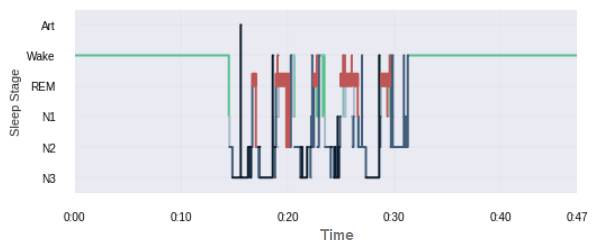
\includegraphics[width=0.80\textwidth]{hipnoHipno} \caption{Hipnogrammas faila SC4001EC-Hypnogram.edf grafisks attēlojums}
\label{hypnoGramS} 
\end{figure}


\subsubsection{Apmācību un testa dati}

Balstoties uz hipnogrammu un to attiecīgo EFD failu datiem tika paņemti EEG Fpz-Cz un EEG Pz-Oz signāli, kas tika sadalīti pa apakšsignāliem. Apakšsignālu garums ir 3000x2, jo hipnogrammas iztveršanas frekvence ir 0.03 un katram šādam intervālam pēc hipnogrammas datiem tiek piešķirta konkrēta miega fāze. Iegūtie signāli tika sadalīti pa attiecīgajām klasēm, kur katra klase atbilst konkrētai miega fāzei. 

Balstoties uz dotās informācijas no hipnogrammam, par miega fāžu sadalījumu, tīkla apmācīšanai tikai ņemti 500 EEG signālu paraugi ar izmēru 3000x2, kas atbilst konktētām miega fāzēm atšķirīgos laika momentos. Šie paraugi tika ņemti nejaušā secībā no septiņiem EDF failiem. Pēc tam šie paraugi tika sadalīti intervālos ar garumu 500 vai 1000 vai atstāti ar orģinālo garumu 3000. Tas ir atkarīgs kādus gadījumus vēlamies testēt. Ja ņemam ievades datu formu 1000x2, tad tīklam kopā būs 7500 apmācības datu. Kad datu forma ir 500x2 tad apmācības datu kopā būs 15000. Kad ieejas datu forma ir 3000x2 tad kopējie apmācības dati ir 2500.

Tīkla validācijai no atlikušajiem datiem tika ņemti 100 EEG signālu paraugi no katras miega fāzes ar izmēru 3000x2. Arī šie signāli tika sadalīti tādos pašos intervālos, kā norādīts ieejas datu izmērā. Tātad, ja ieejas dati ir 3000x2, tad kopējais validācijas datu skaits ir 500, 1000x2 gadījumā 1500 un 500x2 gadījumā 3000 datu. Apmācības un validācijas datu sadalījumu var apskatīt tabulā \ref{dataTablehhh}.

Testēšanai tiek izmantots viss hipnogrammas fails SC4001EC-Hypnogram.edf un attiecīgais EDF fails SC4001E0-PSG.edf. Abi EEG signāli no EDF faila tiek sadalīti līdzīgos paraugu garumos kā apmācības gadījumā, kur ieejas datu formāts ir 1000x2, 3000x2 un 500x2. Koda piemēru var apskatīt pielikumā 5.. 


\begin{table}[H]
\centering
\caption{}
\captionsetup{justification=centering}
\caption*{\textbf{Apmācības un validācijas datu sadalījums}}
\begin{tabular}{|l|l|l|}
\hline
\multicolumn{1}{|c|}{Ievades datu forma} & Apmācības dati & Validācijas dati \\ \hline
500 x 2 & 15000 & 3000 \\ \hline
1000 x 2 & 7500 & 1500 \\ \hline
3000 x 2 & 2500 & 500 \\ \hline
\end{tabular}
\label{dataTablehhh}
\end{table}

\subsubsection{Datu sagatavošanas metodes}
Turpmākā sadaļā tiks aprakstītas sekojošas funkcijas, kuras tiek izmantotas datu kopas sagatavošanai:

\begin{itemize}
\item retrieveHypnogramData_2v
\item seperateSignalsFromEDF
\item divideSignalInSleepStages
\item getStageTrainingAndValidationData
\end{itemize}

%\begin{itemize}
Pirmā metode $retrieveHypnogramData_2v$, kas atrodama pielikumā 6., ir paredzēta hipnogrammas datu izgūšanai. Kā ieejas datus nepieciešams padot mainīgo \textit{path_to_hypno}, kas ir hipnogrammas faila atrašanās vieta un mainīgo \textit{path_to_datafile}, kas ir attiecīgās hinpogrammas EDF fails, kas satur EEG signālu informāciju. Metode \textit{read_hypno}, kas ņemta no Visbrain Sleep bibliotēkas, atgriež mainīgo data, kas satur vērtības no 0 līdz 5, kuras atbilst konkrētai miega fāze (0-"Nomoda", 1 -"N1", 2-"N2", 3-"N3", 4-"REM", 5-"Art"). 5 klase, kas šajā gadījumā ir artefakti, netiek ņemta vērā tīkla apmācīšanā un testēšanā. Un mainīgais $sf$, kas tiek atgriezts, ir iztveršanas frekvence, tā ir svarīga, lai būtu zināms, cik liels ir viena parauga izmērs. 
 
%\begin{lstlisting}[language=Python]
%def retrieveHypnogramData_2v(path_to_hypno, path_to_datafile):
%    data, sf = read_hypno(path_to_hypno,datafile=path_to_datafile)
%    return data,sf
%\end{lstlisting}

Otrā metode $seperateSignalsFromEDF$, kas atrodama pielikumā 6., atgriež datu struktūru ar vienu kolonu $Signal$ un divām rindām, pirmā satur Fpz-Cz un otrā satur Pz-Oz signālu. Kā ieejas datus arī nepieciešams padot manīgo $datafile$, kas ir EDF faila, kas satur EEG signālu informāciju. Mainīgais $n$ tiek nodefinēts kā 2, jo no faila nepieciešams nolasīt tikai Fpz-Cz un EEG Pz-Oz signālus. Lai ielasītu informāciju no EDF faila tiek izmantota $pyedflib$ bibliotēkas metode $EdfReader$. Tālāk tiek izveidota jauna datu struktūra $eegSignals$ ar vienu kolonu, kur glabās EEG signālu informāciju. Nākošais solis ir izgūt signālus no ielasītā faila. Ciklā no faila tiek nolasīta attiecīgā signāla informācija izmantojot readSignal metodi un šī metode atgriež masīvu ar attiecīgā signāla vērtībām. Šo masīvu saglabā izveidotajā datu struktūrā. Kad tiek iegūti abu signālu dati, fails tiek aizvērts un mainīgais $d$ tiek izdzēsts. $eegSignals$ tiek atgriezts. 

%\begin{lstlisting}[language=Python]
%def seperateSignalsFromEDF(datafile):
%    d = edf.EdfReader(datafile)
%    n = 2
%    eegSignals = pd.DataFrame(columns=[['Signal']],index=range(n))
%    
%    for i in np.arange(n):
%        sigbuf= d.readSignal(i)
%        print(d.getSignalLabels())
%        eegSignals.loc[i].Signal=[sigbuf]
%    d._close()
%    del d
%    return eegSignals
%\end{lstlisting}

 Trešajai metodei $divideSignalInSleepStages$, atrodama pielikumā 6., tiek padots mainīgais \textit{sleep_stages}, kas satur hipnogrammas datus un mainīgais \textit{sleep_signal}, kas satur EEG signāla datus. Pirmais solis ir iegūt parauga izmēru, mainīgo $chunks$ aprēķina kopējo signāla garumu dalot ar hipnogrammas kopējo elementu skaitu. Mainīgais $step$ ir sākuma pozīcija un tas tiek inicializēts kā 0. Mainīgais $nextStep$ ir beigu pozīcija. Tālāk nodefinē datu struktūru \textit{data_set}, ar divām kolonām. $Signal$ kolona saturēs apakšsignālu informācija un $Class$ kolona saturēs informāciju par to, kurai miega stqadījai pieder konkrētais apakšsignāls. Tālāk ciklā tiek iets cauri hipnogrammas datiem. Mainīgais $subsignal$ saturēs apakšsignālu, kurš tiek ņemts no kopējā signāla, pēc noteikta intervāla. Intervāla sākumu nosaka manīgais step un beigu pozīciju nosaka mainīgais $nextStep$. Sākuma pozīcija tagad ir beigu pozīcija un jaunā beigu pozīcija ir sākuma pozīcija, kam pieskaitīts mainīgais $chunks$. Mainīgais $signal_with_stage$ saturēs masīvu ar apakšsignāla vērtībām un tālāk šis masīvs tiek saglabāts datu struktūrā \textit{data_set}, kā arī hipnogrammas elements, kas apzīmē miega stadīju, arī tiek saglabāts šajā datu struktūrā. Kad tiek iziets cauri visiem hipnogrammas elementiem, tiek atgriezta datu struktūra \textit{data_set}, kas satur apakšsignālu un to miega fāžu informāciju.

%\begin{lstlisting}[language=Python]    
%def divideSignalInSleepStages(sleep_stages,sleep_signal):
%    chunks = len(sleep_signal)//len(sleep_stages)
%    step = 0
%    nextStep = int(step+chunks)
%    data_set = pd.DataFrame(columns=[['Class','Signal']]    ,index=range(len(sleep_stages)-1))
%    for i in range(len(sleep_stages)-1):
%        subsignal = sleep_signal[step:nextStep]
%        step = nextStep
%        nextStep=step+chunks
%        signal_with_stage = np.array(subsignal)
%        data_set.loc[i].Class = int(sleep_stages[i])
%        data_set.loc[i].Signal=[signal_with_stage]
%    return data_set  
%\end{lstlisting}


Ceturtā metode $getStageTrainingAndValidationData$, kas atrodama pielikumā 6., ir paredzēta testa, apmācības un validācijas datu kopu sagatavošanai. \textit{signal_data1} mainīgais ir pirmā kanāla EEG signāla dati, $signal_data2$ mainīgais ir otrā kanāla EEG signāla dati. $classOfSamples$ mainīgais apzīmē, kuras miega fāzes datus vēlamies sadalīt . $traingSize$ mainīgais apzīmē to cik daudz datu tiks izmantots tīkla apmācībai, $testSize$ mainīgais apzīmē to cik daudz datu tiks izmantots tīkla testēšanai un $validationSize$ mainīgais apzīmē to cik daudz datu tiks izmantots tīkla validācijai. Sākumā tiek nodefinētas datu struktūras \textit{eeg_test}, kas saturēs testa datus,\textit{eeg_val}, kas saturēs validācijas datus un \textit{eeg_train}, kas saturēs apmācības datus. Tiek arī nodefinēta datu struktūra $temp$, kas saturēs konkrētu signālu datus. Ciklā tiek iets cauri visiem pirmā kanāla signāliem. Tiek izgūta miega fāze un abu kanālu signālu dati, kas pēc tam tiek saglabāti datu struktūrā $temp$. Un pēc tam tiek veikta \textit{eeg_test},\textit{eeg_val} un \textit{eeg_train} izmēru pārbaude, lai zinātu vai datu struktūrām var pievienot vēl vienu rindu ar datiem. Pēc tam, kad ir iziets cauri visiem kanāla signāliem, tiek atgrieztas šīs datu struktūras, kuras pēc tam tiks padotas izveidotajam partiju (no angļ. batch) ģenerātoram. 
  
%  \begin{lstlisting}[language=Python]
%def getStageTrainingAndValidationData(signal_data1,signal_data2, 
%classOfSamples,traingSize,testSize,validationSize):
%    eeg_test = pd.DataFrame(columns=[['Class', 'Signal']])
%    eeg_val = pd.DataFrame(columns=[['Class', 'Signal']])
%    eeg_train = pd.DataFrame(columns=[['Class', 'Signal']])
%    temp = pd.DataFrame(columns=[['Class', 'Signal']], index=range(1))

%    for i in range(len(signal_data1)- 1):
%        clas = signal_data1.iloc[i]['Class']
%        sig = signal_data1.iloc[i]['Signal']
%        sig2 = signal_data2.iloc[i]['Signal']
%        temp.loc[0].Class = clas[0]
%        temp.loc[0].Signal = [[sig[0], sig2[0]]]
%        if clas[0] == classOfSamples:

%            if len(eeg_test)<testSize:
%                frames = [eeg_test, temp]
%                eeg_test = pd.concat(frames)
%            elif len(eeg_val)<validationSize:
%                frame = [eeg_val, temp]
%                eeg_val = pd.concat(frame)
%            elif len(eeg_train)<traingSize:
     %           frames = [eeg_train, temp]
    %            eeg_train = pd.concat(frames)
   % return eeg_train,eeg_test,eeg_val  
  
  %\end{lstlisting}

    
% \end{itemize}

\subsubsection{Tīkla apmācīšana}  
  
Balstoties uz pamācību \cite{tutoriA} tika izveidots, partiju (no angļ. batch) ģenerātors. Šis ģenerātors tiek lietots, lai ģenerētu datu kopu uz vairākiem kodoliem reālajā laikā un izmantojot šo ģenerātoru ir iespējams padot izveidoto datu kopu uzreiz izveidotajam tīkla modelim, tādā veidā samazinot atmiņas patēriņu. Turpmākā sadaļā tiks aprakstītas sekojošas funkcijas, kuras tiek izmantotas tīkla apmācībā:

\begin{itemize}
\item __data_generation
\item reshape
\item to_categorical
\item MyDatGen
\item ModelCheckpoint
\item model.fit_generator
\end{itemize}


Partiju ģenerātora izejas kodā bija nepieciešams pārveidot\textit{__data_generation} metodi, lai šī metode spētu izveido datu partijas no sagatavotās datu kopas signāliem, kas tiks padotas tīklam.
Pielāgoto metodi iespējams apskatīt pielikumā 6.. 

Kā ieejas datus nepieciešams padot sarakstu ar indeksiem \textit{list_indexes_temp}, kas apzīmē to, kuras rindas dati tiks ņemti no kopējās datu struktūras $dataSet$. Mainīgais $y$, saturēs miega fāzes jeb klases, sākumā tas ir tukšs masīvs. Mainīgais $chunk$ nosaka cik liels būs apakšsignāls. Mainīgais $parts$ nosaka to cik daļās nepieciešams būs dalīt kopējo signālu. $k$ ir skaitītājs, kas būs nepieciešams, lai sekotu līdz cik daudz apakšsignālu tiek pievienots konkrētajai partijai. $a$ ir mainīgais, kas saturēs iegūtos apakšsignālus no divu kanālu signālu datiem. 

Tālāk tiek ciklā iets cauri indeksiem, lai noteiktu, kurus signālus nepieciešams sadalīt pa apakšsignāliem un iekļaut partijā. $stepOne$ ir sākuma pozīcija, ko inicializē ar $0$. Tiek izgūta konkrēto signālu miega fāze un saglabāta mainīgajā $cl$, kā arī no $dataSet$ tiek izgūti signāli no abiem kanāliem un saglabāti mainīgajā $sig$. 

Tālāk šie signāli tiek izdalīti atsevišķi, $sign$ satur informāciju par pirmā kanāla signālu un $sign2$ satur informāciju par otrā kanāla signālu. 

Nākošais solis ir ciklā iet cauri mainīgajam $parts$, kas nosaka cik daļās jādala šie signāli. Vispirms ir pārbaude vai nav sasniegts partijas atļautais izmērs un pēc tam abu kanālu signāli tiek sadalīti apakšsignālos un saglabāti mainīgajā $a$. Mainīgajā $y$ saglabā attiecīgo signālu miega fāzi. 

Pēc tam nepieciešams iegūto datu kopu pārveidot, lai tā saturētu pareizu dimensiju skaitu. To dara izmantojot metodi $reshape$. \textit{a_new} forma pēc tam būs šāda (signālu skaits, garums, kanāli). \textit{expand_dim} mainīgais nosaka to vai nepieciešams pievienot papildus dimensiju, jo ir tīkla modeļi, kuriem nepieciešams padot datus, kas satur 4 dimensijas nevis trīs. Ja ir nepieciešams pievienot papildus dimensiju, tad izmanto \textit{expand_dims} metodi. \textit{a_new} forma tad izskatītos šādi - (signālu skaits, platums, garums, kanāli). 

Tiek atgriezti iegūtie apakšsignāli un to klases, kas tiek pārveidotas kategoriskā formātā izmantojot metodi \textit{to_categorical}. 

%\begin{lstlisting}[language=Python]
%    def __data_generation(self, list_indexes_temp):
%        # Initialization
%        y = np.empty((self.batch_size), dtype=int)
%        chunk = self.dim[1]
%        parts = int(3000/self.dim[1])
%        k = 0
%        a = np.empty([self.batch_size,self.dim[2],self.dim[1]])
%        # Generate data
%        for i, ID in enumerate(list_indexes_temp):
%            stepOne = 0
%            cl = self.dataSet.iloc[ID]['Class']
%            sig = self.dataSet.iloc[ID]['Signal']
%            si = sig[0]; sign = si[0]; sign2 = si[1]; clas = cl[0]
%            for j in range(parts):
%                if k!=self.batch_size:
%                    a[k,:] = np.array([sign[stepOne:(stepOne +chunk)],sign2[stepOne:(stepOne+chunk)]])
%                    stepOne = stepOne+chunk
%                    y[k] = clas
%                    k = k+1
%                else:
%                    break
        %w = a
        %a_new = np.reshape(w,(w.shape[0],w.shape[2],2))
       % 
      %  if(self.expand_dim):
     %     a_new = np.expand_dims(a_new, axis=1)
    %      
   %     X = a_new
  %      return X, to_categorical(y)
 % \end{lstlisting}
 

  
Kad dati ir sagatavoti, tie vēl ir jāpadod tīklam, lai varētu sākt apmācīt tīklu. Realizāciju kodā var apskatīt pielikumā 6.. 

Vispirms tiek ģenerēts saraksts priekš apmācības datu kopas, kas reprezentē katras rindas indeksu un satur skaitļus no 0 līdz datu kopas izmēram . Nākošais solis ir konvertēt datu struktūras $dataSet$ kolonu, kas satur miega fāzes jeb signālu klases, par sarakstu. To pašu atkārto arī validācijas datu kopai. 
 
Nākošais solis ir izveidot partiju ģeneratoru priekš apmācības un validācijas, ko izmantos apmācot tīklu, izmatojot metodi $MyDatGen$. 
\textit{list_of_Indexes} ir mainīgais , kas satur katras datu kopas rindas indeksu. \textit{batch_size} mainīgais nosaka partijas lielumu. $dataSet$ ir mainīgais, kas satur datu kopu. 

Tiek izveidoti divi partiju ģeneratori. Viens priekš apmācības datiem un otrs priekš validācijas datiem. Parametri, kas jāpadod ir $labels$, kas ir mainīgais, kas satur miega fāzes jeb klases. \textit{expand_dim} ir mainīgais, kas nosaka vai ir nepieciešams ieejas datiem pievienot papildus dimensiju. $dim$ ir mainīgais, kādas būs ieejas datu dimensijas - signālu skaits, garums, kanāli. 


Pirms apmācīšanas tiek nodefinēts $ModelCheckpoint$, kur parametrs \textit{save_best_only} ir $False$, kas nozīmē, ka netiek saglabāti labākie svari tīkla apmācības laikā, $filepath$ mainīgais nosaka, kurus svarus tīkls izmantos. Pēc tam tiek izsaukts \textit{model.fit_generator}, $model$ ir tīkla arhitektūra, kas tiek izveidota iepriekš, par tīkla arhitektūrām, kuras tiek izmantotas tiks apskatītas tālāk darbā un \textit{fit_generator} metode nosaka to, ka tīkla apmācīšanā tiks izmantoti izveidotie ģeneratori - \textit{tra_generator}, \textit{val_generator}. Metodes mainīgais $epochs$ nosaka cik daudz epohu tiks apmācīts, $generator$ mainīgais nosaka kāds būs apmācības datu ģenerators, \textit{validation_data} mainīgais nosaka kādu validācijas ģeneratori izmantos.

Tīkla apmācīšanai tikai ņemti 500 EEG signālu paraugi no katras miega fāzes ar izmēru 3000x2. Šie paraugi tika ņemti nejaušā secībā no septiņiem EDF failiem. Pēc tam šie paraugi tika sadalīti intervālos ar garumu 500 vai 1000 vai atstāti ar orģinālo garumu 3000. Tas ir atkarīgs kādus gadījumus vēlamies testēt. Ja ņemam ievades datu formu 1000x2, tad tīklam kopā būs 7500 apmācības datu. Kad datu forma ir 500x2 tad apmācības datu kopā būs 15000. Kad ieejas datu forma ir 3000x2 tad kopējie apmācības dati ir 2500. 

Tīkla validācijai no atlikušajiem datiem tika ņemti 100 EEG signālu paraugi no katras miega fāzes ar izmēru 3000x2. Arī šie signāli tika sadalīti tādos pašos intervālos, kā norādīts ieejas datu izmērā. Tātad, ja ieejas dati ir 3000x2, tad kopējais validācijas datu skaits ir 500, 1000x2 gadījumā 1500 un 500x2 gadījumā 3000 datu. 

Testēšanai tiek izmantots viss hipnogrammas fails SC4001EC-Hypnogram.edf un attiecīgais EDF fails SC4001E0-PSG.edf. Abi EEG signāli no EDF faila tiek sadalīti līdzīgos paraugu garumos kā apmācības gadījumā, kur ieejas datu formāts ir 1000x2, 3000x2 un 500x2. Koda piemēru var apskatīt pielikumā 5.. 

  %\begin{lstlisting}[language=Python]  
%list_of_indexes = np.arange(0,dataSet.shape[0],1)
%  labels = dataSet['Class'].values.tolist()
%  list_of_val_index = np.arange(0,validDataSet.shape[0],1)
%  labels_val = validDataSet['Class'].values.tolist()

 % tra_generator = MyDatGen(list_of_Indexes=list_of_indexes,batch_size=batch_size ,dataSet=dataSet,labels=labels, expand_dim = expand, dim =dim_shape)
  %val_generator = MyDatGen(list_of_Indexes=list_of_val_index,batch_size=batch_size,
  %dataSet=validDataSet,labels=labels_val, expand_dim = expand,dim =dim_shape)
  %checkpointer = ModelCheckpoint(filepath = weights_name, verbose = 1, save_best_only = False)
  %hist = model.fit_generator(epochs = epochs, generator=tra_generator,validation_data=val_generator,
  %use_multiprocessing=True,workers=0)
   % \end{lstlisting}
  
 
\section{Apmācības modeļi}

Darbā tiek apskatītas dažādas tīkla arhitektūras - LSTM \ref{lstmarch}, CNN \ref{cnnmarch}, CNN ar 2 konvolūcijas slāņiem, kas apvienots ar LSTM \ref{cnn2lstmarch} un CNN ar 8 slāņiem, kas apvienots ar LSTM \ref{cnn8lstmarch}. Gadījumi kad tiek definēti CNN slāņi, izmantojot \textit{Keras} bibliotēku, tiek izmantoti 1D konvolūcijas slāņi. CNN ir vienādas iezīmes un ievēro to pašu pieeju, neatkarīgi no tā, vai tas ir 1D, 2D vai 3D. 

CNN-2 - LSTM un CNN-8 - LSTM ievades dati ir 3D tenzors ar formu: (partijas izmērs, parauga lielums, kanāli). Šajā gadījumā partijai būs vērtība 1, parauga lielums būs piemēram 500 un tiks izmantoti 2 kanālu dati. CNN un LSTM gadījumā ievades dati būs 2D (parauga lielums, kanāli), piemēram, 2 kanālu dati, kur parauga izmērs ir 500. Katrs šāds laika intervāls satur informāciju par pacientu EEG datiem konkrētā miega fāzē.

Izmantojot hibrīda CNN-LSTM modeli, katru paraugu sadala tālākās apakšgrupās. CNN modelis izgūs īpašības no katras apakšgrupas, un LSTM apkopos īpašības no šīm apakšgrupām. Šajā gadījumā viss CNN modelis tiek iesaiņots Laikā Sadalītos (angļ. TimeDistributed) slāņos tā, lai to varētu piemērot katrai parauga apakšgrupai. Katrs ievades datu laika intervāls tiek iesaiņots un pēc tam LSTM slānis apkopo rezultātus, pirms modelis atgriež prognozētos klašu datus.

CNN, CNN-2 - LSTM un CNN-8 - LSTM modeļiem konvolūcijas pirmā slāņa filtra augstums tīkliem ir 3. To sauc arī par kodola lielumu. Ja tiktu definēts tikai viens filtrs, neironu tīkls pirmajā slānī varētu apgūt vienu īpašību no datiem. Tas var nebūt pietiekams, tāpēc jānodefinē lielāks filtru skaits, piemēram, 16 filtri. Tas ļauj  pirmajā tīkla slānī apmācīt 16 dažādas īpašības. Pirmā neironu tīkla slāņa izejas dati ir 498x16 neironu matrica. Katra izejas datu matricas kolonna satur viena filtra svarus. Ar nodefinēto kodola lielumu un, ņemot vērā ievades matricas garumu, katrs filtrs satur 498 svarus. Un kā aktivizēšanas funkcija tiek izmantota ReLU.

Lai samazinātu izejas datu sarežģītību un novērstu to, ka tīkls pārmācās. Pēc CNN slāņa tiks izmantots apvienošanas slānis. Šajā gadījumā tiks izmantoti maksimālās apvienošanas slāņi ar filtriem, kuru dimensionalitāte ir 2x2. Pēc konvolūcijas slāņa ir iespējams arī pievienot partijas normalizēšanu, kas mazina dažādu slāņu ieeju ietekmi. Normalizējot neironu izvadi, aktivizēšanas funkcija saņems tikai ieejas datus, kas ir tuvu nullei. Tas ir arī risina izzūdošā gradienta problēmu.  

Tīkliem izmantos gan Izslēgšanas (no angļ. Dropout) un Telpiskās izslēgšanas (no angļ. Spatial Droput) slāņus. Izslēgšanas ir regulēšanas metode, ko patentē Google, lai samazinātu neironu tīklu pārmācīšanos, novēršot to, ka rodas sarežģīta savstarpējā pielāgošanās apmācības datos. Tas ir ļoti efektīvs veids, kā ar neironu tīkliem veikt modeļa vidējošanu (no angļ. averaging). Izslēgšanas slānis piešķir nejauši izvēlētiem svariem 0 vērtību. 

Telpiskās izslēgšanas slānis veic tādu pašu funkciju kā Izslēgšanas, tomēr tā vietā, lai samazinātu atsevišķu elementu svarus tiek atmesta visa 1D īpašību karte. Izmantojot šo darbību, tīkls kļūst mazāk jutīgs pret mazām datu izmaiņām. Ja īpašību kartēs blakus esošie kadri ir cieši saistīti, tad izslēgšana neregulēs aktivizāciju bet tikai izraisīs efektīvu mācīšanās ātruma samazināšanos.

Kā arī tīkla arhitektūras tiks izmantots izlīdzināšanas slānis. Izlīdzināšana nozīmē to ,ka tiks samazinātas dimensijas tā, lai paliktu tikai viena dimensija. Izlīdzināšanas slānis pārveido tenzoru tā lai izveidotos tāda formu, kas ir vienāda ar tenzora elementu skaitu jeb viendimensionāls masīvs ar visiem elementiem. 

LSTM modelim pirmais LSTM slānis izmanto parametru "return_sequences" ar vērtību "True", kas nosaka to vai izejas dati būs tādā pat formātā kā pēdējie ieejas dati vai arī tiks atgriezts 1D vektors. 

Katra tīkla beigās ir pilnībā savienotais slānis, kas veic klasifikāciju pēc īpašībām, kuras tiek izgūtas no konvolūcijas slāņiem un samazinātas (angļ. val. downsampled) izmantojot apvienošanas slāņus. Pilnībā savienotajā slānī katrs slāņa neirons ir savienots ar katru iepriekšējā slāņa neironu.

Pēdējais slānis samazina ieejas vektora garumu uz piecu elementu vektoru, jo izejas dati ir piecas klases, kuras vēlas paredzēt ("Wake", "REM", "N1", "N2", "N3"). Sigmoid tiek izmantots kā aktivizēšanas funkcija. Izejas dati tiek pārveidoti tā, lai sasummējot visu piecu klašu vērtības kopā gala rezultāts būt viens. Tādējādi izejas vērtība atspoguļo varbūtību katrai no piecām klasēm, kas šajā gadījumā ir miega fāzes.

%\subsection{LSTM}
\begin{figure}[H] \centering
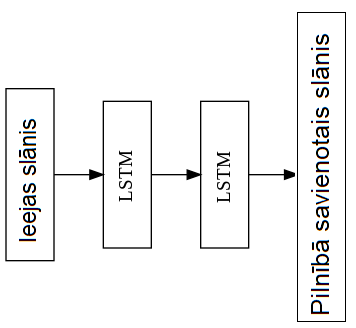
\includegraphics[width=0.40\textwidth]{CNNLSTMtikls} \caption{LSTM tīkla arhitektūra}  
\label{lstmarch} 
\end{figure}

%\subsection{CNN}
\begin{figure}[H] \centering
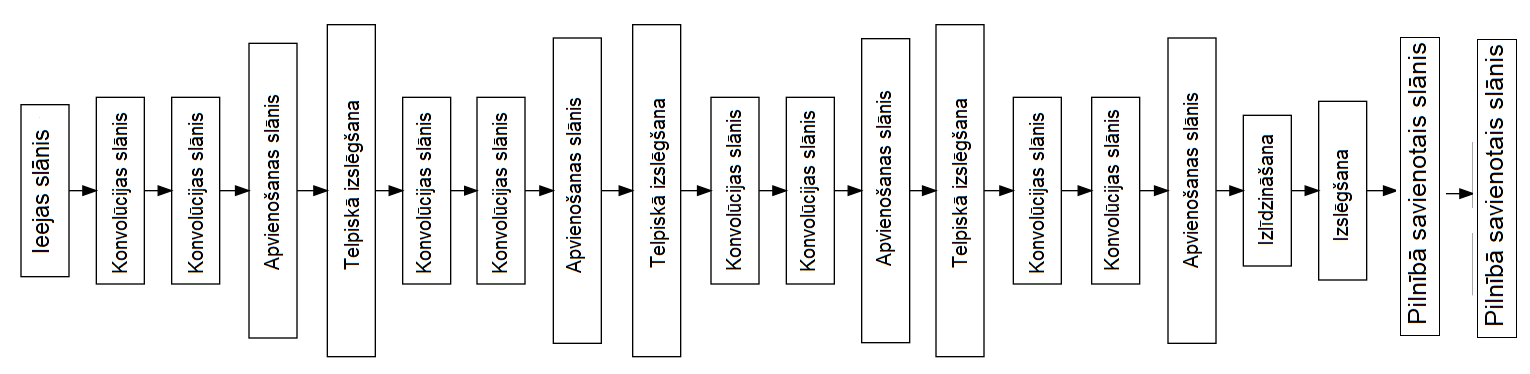
\includegraphics[width=1.05\textwidth]{CNNtikls} \caption{CNN tīkla arhitektūra} 
\label{cnnmarch} 
\end{figure}

%\subsection{CNN-2 - LSTM}
\begin{figure}[H] \centering
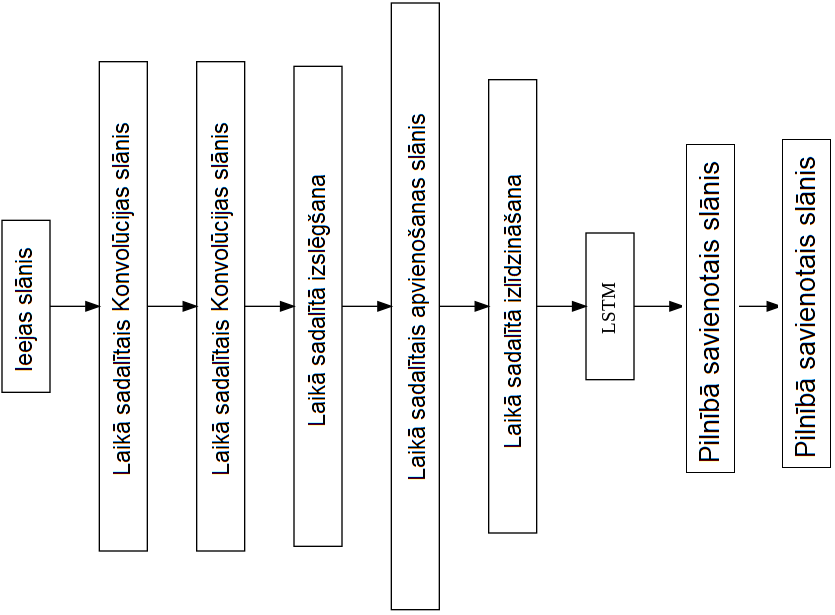
\includegraphics[width=0.70\textwidth]{CNN2LSTMtikls} \caption{CNN-2 - LSTM tīkla arhitektūra}  
\label{cnn2lstmarch} 
\end{figure}

%\subsection{CNN-8 - LSTM}
\begin{figure}[H] \centering
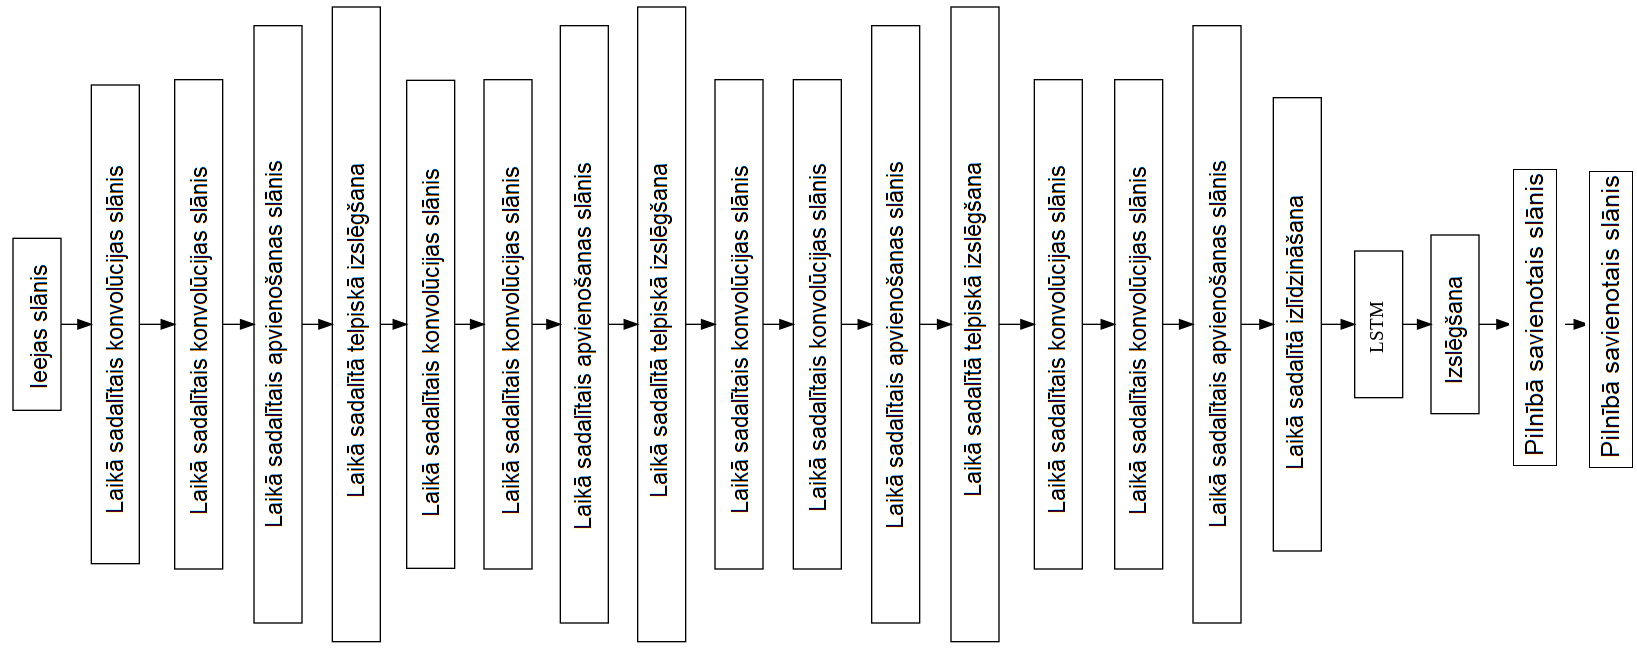
\includegraphics[width=1.05\textwidth]{CNN8LSTMtikls} \caption{CNN-8 - LSTM tīkla arhitektūra}  
\label{cnn8lstmarch} 
\end{figure}


\section{Rezultātu novērtēšanas metrikas}
%\begin{itemize}

\textbf{Korelācijas koeficients} ir skaitlisks mērījums kādam korelācijas veidam, kas nozīmē statistisko sakarību starp diviem mainīgajiem. Mainīgie lielumi var būt divas kolonas no novērojumu datu kopas, ko bieži sauc par paraugiem, vai divas daudzfaktoru gadījumu izlases mainīgās komponentes ar zināmu sadalījumu. Ja attiecība starp mainīgajiem nav lineāra, tad korelācijas koeficients nepietiekami atspoguļo attiecību starp mainīgajiem lielumiem.
Pozitīva korelācija nozīmē to, ka vienam manīgajam palielinoties arī otrs palielinās. Negatīva korelācija nozīmē to, ka vienam mainīgajam palielinoties otrs samazinās. Ja nav korelācijas tad arī nav saistības starp abu mainīgo izmaiņām. Korelācijas spēks nozīmē to, ka, jo tuvāk absolūtā vērtība -1 vai 1, jo spocīgāka ir korelācija.
Saikni starp korelācijas koeficienta matricu corr, kovariācijas matricu C un standartnovirzi $\sigma$ datu kopai $\hat{y}$ un $y$ nosaka vienādojums \ref{eq:covForm}.

\begin{equation}
corr = {\frac {C(Y, \hat{Y})}{\sigma_y \sigma_{\hat{y}} }} 
\label{eq:covForm}
\end{equation}
Atkarībā no $corr$ vērtības tiek noteiks cik stipra ir korelācija starp divām  datu kopām. Ja $0 = |corr|$ tad korelācijas neeksistē, ja $0<|corr|<0.2$ tad pastāv ļoti vāja korelācija. Ja $0.2 \leq |corr| <0.4$ tad pastāv vāja korelācija. Ja $0.4 \leq |corr|<0.6$ tad pastāv mēreni spēcīga korelācija.
Ja $0.6 \leq |corr| \leq 0.8$ tad pastāv spēcīga korelācija
Kad $0.8 \leq |corr| <1.0$ tad ir ļoti spēcīga korelācija un ja  $1.0 = |corr|$ tad ir ideāla korelācija. \\

%https://study.com/academy/lesson/pearson-correlation-coefficient-formula-example-significance.html	 

 %http://faculty.cas.usf.edu/mbrannick/regression/corr1.html

\textbf{Vidējā kvadrāta kļūda} mēra prognozes vidējo kvadrāta kļūdu. Katram punktam tā aprēķina kvadrātisko starpību starp prognozētajiem un patiesajiem datiem un pēc tam iegūst vidējo vērtību starp abiem lielumiem. MSE aprēķina pēc formulas \ref{eq:mseE}. Jo augstāka šī vērtība, jo sliktāks ir modelis. Šī kļūda nekad nepieņem negatīvu vērtību, jo pirms summēšanas individuālās prognozēšanas kļūdas tiek celtas kvadrātā. Perfektam modelim šī vērtība būs nulle. \\


\textbf{Pārpratuma matrica} ir tabula \ref{confMat}, ko bieži izmanto, lai aprakstītu klasifikācijas modeļa veiktspēju un tā satur 4 dažādas paredzamo un faktisko vērtību kombinācijas.


\begin{figure}[H] \centering
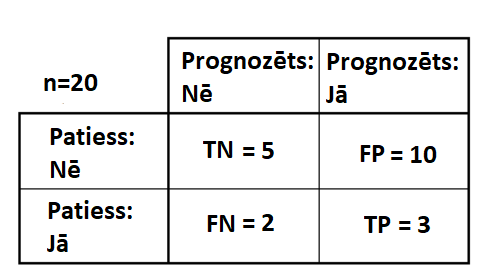
\includegraphics[width=0.45\textwidth]{confmat} 
\caption{Pārpratuma matrica} \cite{bptt}  \label{confMat} 
\end{figure}

\begin{itemize}
\item TP - Pareiza atbilsme ir rezultāts, kurā modelis pareizi prognozē pozitīvo klasi.

\item FP - Kļūdaina atbilsme ir rezultāts, kurā modelis nepareizi prognozē pozitīvo klasi. 

\item TN - Pareiza neatbilsme ir rezultāts, kurā modelis pareizi prognozē negatīvo klasi.

\item FN - Kļūdaina neatbilsme ir rezultāts, kurā modelis nepareizi prognozē negatīvo klasi.
\end{itemize}


%https://heartbeat.fritz.ai/5-regression-loss-functions-all-machine-learners-should-know-4fb140e9d4b0

 \textbf{Precizitāte} ir viena metrika klasifikācijas modeļu novērtēšanai. Precizitāte ir tā daļa no prognozētajiem datiem, kuru modelim bija pareizi atpazinis. Precizitāte palīdz veikt datu analīzi, lai iegūtu vairāk ieskatu par modeļa veiktspēju. Formāli precizitātes formula ir \ref{eq:writtenPos}, kur $n$ ir kopējais paraugu skaits, $\hat{y}$ ir prognozētie dati un $y$ ir patiesie dati.
 
\begin{equation}
acc = \frac{1}{n} \sum_{i=0}^{n-1} 1(\hat{y_i}=y_i)
\label{eq:writtenPos}
\end{equation}\\

 \textbf{$F_1$ novērtējums (no angļ. $F_1$ score)} nosaka tīkla precizitāti kad tiek veikta testēšana. Lai aprēķinātu šo novērtējumu izmanto formulu \ref{eq:truePozitive}. Lai aprēķinātu rezultātu, tiek ņemta vērā gan precizitāte p, gan testa atsauksme r. Precizitāte ir pareizo atbilsmju skaits, kas dalīts ar kopējo pareizo atbilsmju un kļūdaino atbilsmju skaitu. Atsauksme ir pareizo atbilsmju skaits, kas dalīts ar kopējo pareizo atbilsmju skaitu un kļūdaino neatbilsmju skaitu. Vērtība 1 apzīmē labāko un 0 apzīmē sliktāko gadījumu.

\begin{equation}
F_1 = 2 * \frac{p*r}{p + r}
\label{eq:truePozitive}
\end{equation}

%Binārajai klasifikācijai precizitāti var aprēķināt arī pēc pozitīviem un negatīviem gadījumiem izmantojot formulu \ref{eq:truePozitive} balstoties uz pārpratuma matricas vērtībām. 

%\begin{equation}
%Precizitāte = \frac{TP + TN}{TP + TN + FP + FN}
%\label{eq:truePozitive}
%\end{equation}
%\end{itemize}





%https://developers.google.com/machine-learning/crash-course/classification/accuracy
%https://www.ncbi.nlm.nih.gov/pmc/articles/PMC4614595/

%\section{Tīkla uzlabošanas metodes}

\chapter{Rezultāti}
% Please add the following required packages to your document preamble:
% \usepackage[table,xcdraw]{xcolor}
% If you use beamer only pass "xcolor=table" option, i.e. \documentclass[xcolor=table]{beamer}

\subsubsection*{Klasifikācija izmantojot 2 klases}


Veicot detalizētāku datu kopas izpēti redzam, ka nomodas dati proporcionāli ir daudz vairāk, nekā miega dati. Autore ir ieinteresēta tieši miega fāžu noteikšanai. Šī iemesla dēļ vispirms tiks veikta nomodas un kopējās miega fāzes klasifikācija. Tas tika darīts, lai būtu iespējams izvērtēt vai modeļi vispār spēj atpazīt momentus, kad cilvēks ir nomodā vai arī cilvēks ir aizmidzis. Apmācībai dati tika ņemti no viena EDF faila SC4001E0-PSG.edf un tā pavadošās hipnogrammas SC4001EC-Hypnogram.edf. 


Iegūtās pārpratuma matricas \ref{tabcoda}, \ref{tarv} procentuāli apzīmē, cik pareizi un nepareizi tika klasificētas miega un momoda fāzes, kad datu izmērs ir 500x2 un 50 epohām.
No Nomoda fāzes klasifikācijai tika paņemti 3258 paraugi un no miega fāzes tika ņemti 3309 paraugi.  


CNN modeļa gadījumā var redzēt, ka tikai 6\% (202) no visiem miega fāzes paraugiem tika klasificēti kā Nomoda fāzes paraugi. Līdzīgi arī ir CNN-2 - LSTM modelim Miega paraugu klasifikācijas gadījumā. CNN-8 - LSTM par 1\% (3136) labāk izdevās klasificēt miega fāzes paraugus, bet LSTM modeļa kļūda ir 7\% (228). 

Apskatot Nomoda klasifikāciju, situācija ir mazliet sliktāka. CNN pareizi izdevās klasificēt 71\% (2073) no visiem Nomoda fāzes paraugiem, CNN-2 - LSTM gadījumā 72\% (2078) izdevās klasificēt korekti. Labākais rezultāts ir CNN-8 - LSTM, kam izdevās klasificēt 74\% (2083) korekti, bet LSTM modelim tikai 63\% (2068) izdevās klasificēt korekti, kas ir par apmēram 10 \% sliktāk nekā pārējiem 3 modeļiem.



\begin{table}[H]
\centering
\caption{}
\captionsetup{justification=centering}
\caption*{\textbf{Pārpratuma matricas}}
\begin{tabular}{lccllccllcc}
 & \multicolumn{2}{c}{CNN} &  &  & \multicolumn{2}{c}{CNN-2 - LSTM} &  &  & \multicolumn{2}{c}{CNN-8 - LSTM} \\ \cline{2-3} \cline{6-7} \cline{10-11} 
\multicolumn{1}{l|}{} & \multicolumn{1}{c|}{Nomoda} & \multicolumn{1}{c|}{Miega} &  & \multicolumn{1}{l|}{} & \multicolumn{1}{c|}{Nomoda} & \multicolumn{1}{c|}{Miega} &  & \multicolumn{1}{l|}{} & \multicolumn{1}{c|}{Nomoda} & \multicolumn{1}{c|}{Miega} \\ \cline{1-3} \cline{5-7} \cline{9-11} 
\multicolumn{1}{|c|}{Nomoda} & \multicolumn{1}{c|}{\cellcolor[HTML]{FFFFC7}2073} & \multicolumn{1}{c|}{1185} & \multicolumn{1}{l|}{} & \multicolumn{1}{c|}{Nomoda} & \multicolumn{1}{c|}{\cellcolor[HTML]{FFFFC7}2078} & \multicolumn{1}{c|}{1180} & \multicolumn{1}{l|}{} & \multicolumn{1}{c|}{Nomoda} & \multicolumn{1}{c|}{\cellcolor[HTML]{FFFFC7}2083} & \multicolumn{1}{c|}{1175} \\ \cline{1-3} \cline{5-7} \cline{9-11} 
\multicolumn{1}{|c|}{Miega} & \multicolumn{1}{c|}{202} & \multicolumn{1}{c|}{\cellcolor[HTML]{FFFFC7}3107} & \multicolumn{1}{l|}{} & \multicolumn{1}{c|}{Miega} & \multicolumn{1}{c|}{183} & \multicolumn{1}{c|}{\cellcolor[HTML]{FFFFC7}3126} & \multicolumn{1}{l|}{} & \multicolumn{1}{c|}{Miega} & \multicolumn{1}{c|}{173} & \multicolumn{1}{c|}{\cellcolor[HTML]{FFFFC7}3136} \\ \cline{1-3} \cline{5-7} \cline{9-11} 
\end{tabular}
\label{tabcoda}
\end{table}

% Please add the following required packages to your document preamble:
% \usepackage[table,xcdraw]{xcolor}
% If you use beamer only pass "xcolor=table" option, i.e. \documentclass[xcolor=table]{beamer}
\begin{table}[H]
\centering
\caption{}
\captionsetup{justification=centering}
%\caption*{\textbf{Pārpratuma matricas}}
\begin{tabular}{lcc}
 & \multicolumn{2}{c}{LSTM} \\ \cline{2-3} 
\multicolumn{1}{l|}{} & \multicolumn{1}{c|}{Nomoda} & \multicolumn{1}{c|}{Miega} \\ \hline
\multicolumn{1}{|c|}{Nomoda} & \multicolumn{1}{c|}{\cellcolor[HTML]{FFFFC7}2068} & \multicolumn{1}{c|}{1180} \\ \hline
\multicolumn{1}{|c|}{Miega} & \multicolumn{1}{c|}{228} & \multicolumn{1}{c|}{\cellcolor[HTML]{FFFFC7}3030} \\ \hline
\end{tabular}
\label{tarv}
\end{table}


Pārpratuma matricas \ref{1000V2cl}, \ref{1000VV2fasd} procentuāli apzīmē, cik pareizi un nepareizi tika klasificētas miega un Nomoda fāzes, kad datu izmērs ir 1000x2. No Nomoda fāzes klasifikācijai tika paņemti 2066 paraugi un no miega fāzes tika ņemti 1956 paraugi.

Salīdzinājumā ar iepriekš apskatītājām pārpratuma matricām \ref{tabcoda}, \ref{tavsDSSS}, precizitāte pie datu izmēra 1000x2 uzlabojas. Šajā gadījumā CNN miega fāzea paraugus atpazīst ar 98\% (1926) precizitāti. Līdzīgi kā iepriekš, CNN-2 - LSTM iegūst par vienu 1\% (1940) labāku rezultātu, bet pats labākais rezultāts ir CNN-8 - LSTM, kas spēja 100\%(1955) noteikt miega fāzes no Nomoda fāzi. LSTM spēja atpazīt korekti 88\% (1727) no miega fāzes paraugiem. 

Apskatot Nomoda fāzes paraugus, CNN spēja pareizi klasificēt 85\% (1756), CNN-2 - LSTM 82\% (1686). CNN-8 - LSTM, līdzīgi kā CNN, korekti klasificēja 85\% (1754), bet, kā redzams LSTM gadījumā, modelis spēja pareizi noteikt 65\% no visiem paraugiem.


\begin{table}[H]
\centering
\caption{}
\captionsetup{justification=centering}
\caption*{\textbf{Pārpratuma matricas}}
\begin{tabular}{lccllccllcc}
 & \multicolumn{2}{c}{CNN} &  &  & \multicolumn{2}{c}{CNN-2 - LSTM} &  &  & \multicolumn{2}{c}{CNN-8 - LSTM} \\ \cline{2-3} \cline{6-7} \cline{10-11} 
\multicolumn{1}{l|}{} & \multicolumn{1}{c|}{Nomoda} & \multicolumn{1}{c|}{Miega} &  & \multicolumn{1}{l|}{} & \multicolumn{1}{c|}{Nomoda} & \multicolumn{1}{c|}{Miega} &  & \multicolumn{1}{l|}{} & \multicolumn{1}{c|}{Nomoda} & \multicolumn{1}{c|}{Miega} \\ \cline{1-3} \cline{5-7} \cline{9-11} 
\multicolumn{1}{|c|}{Nomoda} & \multicolumn{1}{c|}{\cellcolor[HTML]{FFFFC7}1756} & \multicolumn{1}{c|}{310} & \multicolumn{1}{l|}{} & \multicolumn{1}{c|}{Nomoda} & \multicolumn{1}{c|}{\cellcolor[HTML]{FFFFC7}1686} & \multicolumn{1}{c|}{380} & \multicolumn{1}{l|}{} & \multicolumn{1}{c|}{Nomoda} & \multicolumn{1}{c|}{\cellcolor[HTML]{FFFFC7}1754} & \multicolumn{1}{c|}{312} \\ \cline{1-3} \cline{5-7} \cline{9-11} 
\multicolumn{1}{|c|}{Miega} & \multicolumn{1}{c|}{33} & \multicolumn{1}{c|}{\cellcolor[HTML]{FFFFC7}1926} & \multicolumn{1}{l|}{} & \multicolumn{1}{c|}{Miega} & \multicolumn{1}{c|}{19} & \multicolumn{1}{c|}{\cellcolor[HTML]{FFFFC7}1940} & \multicolumn{1}{l|}{} & \multicolumn{1}{c|}{Miega} & \multicolumn{1}{c|}{4} & \multicolumn{1}{c|}{\cellcolor[HTML]{FFFFC7}1955} \\ \cline{1-3} \cline{5-7} \cline{9-11} 
\end{tabular}
\label{1000V2cl}
\end{table}

% Please add the following required packages to your document preamble:
% \usepackage[table,xcdraw]{xcolor}
% If you use beamer only pass "xcolor=table" option, i.e. \documentclass[xcolor=table]{beamer}
\begin{table}[H]
\centering
\caption{}
\captionsetup{justification=centering}
%\caption*{\textbf{Pārpratuma matricas}}
\begin{tabular}{lcc}
 & \multicolumn{2}{c}{LSTM} \\ \cline{2-3} 
\multicolumn{1}{l|}{} & \multicolumn{1}{c|}{Nomoda} & \multicolumn{1}{c|}{Miega} \\ \hline
\multicolumn{1}{|c|}{Nomoda} & \multicolumn{1}{c|}{\cellcolor[HTML]{FFFFC7}1335} & \multicolumn{1}{c|}{731} \\ \hline
\multicolumn{1}{|c|}{Miega} & \multicolumn{1}{c|}{222} & \multicolumn{1}{c|}{\cellcolor[HTML]{FFFFC7}1727} \\ \hline
\end{tabular}
\label{1000VV2fasd}
\end{table}


\subsubsection*{Klasifikācija izmantojot 5 klases}

Balstoties uz labajiem klasifikācijas rezultātiem, kas tika iegūti klasificējot miega un nomodas fāzes, tika nolemts apskatīt datu kopas klasifikāciju ar visām klasēm (Nomoda, N1, N2, N3 un REM). Kā piemērs, tika apskatīti \cite{git1}, \cite{git2}, \cite{git3}. 

Pārpratumu matricām \ref{matrixOfConf}, \ref{matrixOfConf2v} ar dzelteno krāsu tiek atzīmēts, cik paraugu pareizi tiek atpazīti kā attiecīgā miega fāze. Virs matricas ir modeļa nosaukums un pati pārpratuma matricas attēlo, to kā tiek atpazīti EEG signāli 
no katras miega fāzes. Vertikāli tiek attēlotas patiesās miega fāzes un horizontāli tiek attēlotas 
prognozētās miega fāzes. Attiecīgās rindas un kolonas vērtības matricā atspoguļo to, pie kuras miega fāzes tiek klasificēti attiecīgi EEG signāli. Piemēram, ja apskata CNN matricu \ref{matrixOfConf} 
Nomoda fāzi, var redzēt to, ka 215 Nomoda fāzes signāli tika klasificēta, ka tie pieder Nomoda fāzei, 165 Nomoda fāzes signāli tika klasificēti, ka tie pieder N1 fāzei, 38 tika klasificēti kā N2, 12 kā N3 un 104 kā REM miega fāzei piederoši signāli. 

Kopumā testēšanai no hipnogrammas SC4001EC-Hypnogram.edf un attiecīgais EDF fails SC4001E0-PSG.edf tika ņemti 543‬
 Nomoda signāli, ‭348‬ N1 fāzes signāli, 1500 N2 fāzes signāli, 1320 N3 fāzes signāli, 740 REM fāzes signāli, kad ieejas datu izmērs ir 500x2 un epohas ir 50.


LSTM modeļa gadījumā, kad ieejas dati ir 500, var novērot to, ka no visiem paraugiem, kas 
pieder Nomoda fāzei 39\% (210) tiek klasificēti kā piederoši N2 fāzei un 24\% (130) kā piederoši REM fāzei, bet tikai 11\% (62) tiek klasificēti kā Nomoda fāze. ‭

No N1 fāzes paraugiem 31\% (108) tiek uzskatīts par REM fāzes paraugiem, bet tikai 15\% (51) tiek uzskatīti par N1, kā arī N2 fāzes 
paraugi 29\% (432) gadījumu tiek klasificēti kā REM fāzes paraugi un 20\% (293) gadījumu kā N1, bet tikai 26\% (393) gadījumu kā N2. N3 fāzes paraugi tiek uzskatīti par piederošiem 26\% (341) N1 un 25\% (326) REM fāzei, bet pašai N3 fāzei
17\% (226) no visiem N3 fāzes paraugiem. REM fāzes gadījumā, 31\% (226) paraugi tiek uzskatīti par REM un 31\% (226) N2 fāzes paraugiem. 

CNN gadījumā, var novērot to, ka Nomoda fāze pareizi klasificē 40\% (215) bet 30\% (165) tiek klasificēti kā N1 fāzei
un 19\% (104) kā REM fāzei piederoši.
N1 fāzes paraugi lielākoties tiek klasificēti, kā piederoši N2 fāzei ar 46\% (160), bet tikai 18\% (64) tiek klasificēti kā 
N1 fāze. N2 fāzes paraugus modelis 79\% (1188) klasificē korekti un 15\% (225) paraugu klasificē kā N3 fāzes un kā var redzēt N3 fāzes
 gadījumā paraugi 27\% (353) tiek uzskatīti par N2 fāzei piederošiem, bet pašai N3 fāzei 64\% (845). REM fāzes paraugi 44\% (326) gadījumu tiek uzskatīti par N2 fāzes paraugiem, bet kā REM tikai 33\% (247). 


CNN-2 - LSTM gadījumā no Nomoda fāzes paraugiem 43\% (234) tiek klasificēti kā REM fāzes paraugi, bet 42\% (227) kā Nomoda. 
Šajā gadījumā no visiem N1 fāzes paraugiem tikai 1\% (4) tika klasificēts korekti, 
pārējie tiek klasificēti kā citu klašu paraugi, lielākoties 48\% (167) kā REM un 36\% (125) kā N2. Līdzīgi kā CNN gadījumā N2 fāzes paraugi bieži tiek klasificēti kā N3 fāzes paraugi, šajā gadījumā 30\% (443). 60\% (893) tika klasificēti korekti kā N2 fāze. 
N3 fāzes paraugi tiek 9\% (117) gadījumu pieskaitīti pie N2, bet 88\% (1162) tiek klasificēti korekti. No REM fāzes paraugiem 33\% (241) tiek uzskatīti par N2 fāzes signāliem un 63\% (466) tiek uzskatīti korekti par REM. 

CNN-8 - LSTM gadījumā no Nomoda fāzes paraugiem 41\% (221) tiek klasificēti kā REM fāzes paraugi, bet 43\% (235) kā Nomoda. 
Šajā gadījumā no visiem N1 fāzes paraugiem 29\% (100) tika klasificēts korekti un 44\% (154) kā REM fāzes paraugi. 
Līdzīgi kā CNN gadījumā N2 fāzes paraugi bieži tiek klasificēti kā N3 fāzes paraugi, šajā gadījumā 13\% (190). 71\% (1070) tika klasificēti
korekti kā N2 fāze. 
N3 fāzes paraugi tiek 28\% (376) gadījumu pieskaitīti pie N2 un 67\% (896) tiek klasificēti korekti kā N3.
No REM fāzes paraugiem 21\% (155) tiek uzskatīti par N1 fāzei un 67\% (495) tiek uzskatīti korekti par REM. 


\begin{table}[H]
\centering
\caption{}
\captionsetup{justification=centering}
\caption*{\textbf{Pārpratuma matricas}}
\begin{tabular}{cccccclcccccc}
\multicolumn{1}{l}{} & \multicolumn{5}{c}{LSTM} &  & \multicolumn{1}{l}{} & \multicolumn{5}{c}{CNN} \\ \cline{2-6} \cline{9-13} 
\multicolumn{1}{l|}{} & \multicolumn{1}{c|}{Nomoda} & \multicolumn{1}{c|}{N1} & \multicolumn{1}{c|}{N2} & \multicolumn{1}{c|}{N3} & \multicolumn{1}{c|}{REM} &  & \multicolumn{1}{l|}{} & \multicolumn{1}{c|}{Nomoda} & \multicolumn{1}{c|}{N1} & \multicolumn{1}{c|}{N2} & \multicolumn{1}{c|}{N3} & \multicolumn{1}{c|}{REM} \\ \cline{1-6} \cline{8-13} 
\multicolumn{1}{|c|}{Nomoda} & \multicolumn{1}{c|}{\cellcolor[HTML]{FFFFC7}62} & \multicolumn{1}{c|}{58} & \multicolumn{1}{c|}{210} & \multicolumn{1}{c|}{83} & \multicolumn{1}{c|}{130} & \multicolumn{1}{l|}{} & \multicolumn{1}{c|}{Nomoda} & \multicolumn{1}{c|}{\cellcolor[HTML]{FFFFC7}215} & \multicolumn{1}{c|}{165} & \multicolumn{1}{c|}{38} & \multicolumn{1}{c|}{12} & \multicolumn{1}{c|}{104} \\ \cline{1-6} \cline{8-13} 
\multicolumn{1}{|c|}{N1} & \multicolumn{1}{c|}{51} & \multicolumn{1}{c|}{\cellcolor[HTML]{FFFFC7}51} & \multicolumn{1}{c|}{88} & \multicolumn{1}{c|}{50} & \multicolumn{1}{c|}{108} & \multicolumn{1}{l|}{} & \multicolumn{1}{c|}{N1} & \multicolumn{1}{c|}{19} & \multicolumn{1}{c|}{\cellcolor[HTML]{FFFFC7}64} & \multicolumn{1}{c|}{160} & \multicolumn{1}{c|}{21} & \multicolumn{1}{c|}{84} \\ \cline{1-6} \cline{8-13} 
\multicolumn{1}{|c|}{N2} & \multicolumn{1}{c|}{179} & \multicolumn{1}{c|}{293} & \multicolumn{1}{c|}{\cellcolor[HTML]{FFFFC7}393} & \multicolumn{1}{c|}{203} & \multicolumn{1}{c|}{432} & \multicolumn{1}{l|}{} & \multicolumn{1}{c|}{N2} & \multicolumn{1}{c|}{13} & \multicolumn{1}{c|}{40} & \multicolumn{1}{c|}{\cellcolor[HTML]{FFFFC7}1188} & \multicolumn{1}{c|}{225} & \multicolumn{1}{c|}{34} \\ \cline{1-6} \cline{8-13} 
\multicolumn{1}{|c|}{N3} & \multicolumn{1}{c|}{158} & \multicolumn{1}{c|}{341} & \multicolumn{1}{c|}{269} & \multicolumn{1}{c|}{\cellcolor[HTML]{FFFFC7}226} & \multicolumn{1}{c|}{326} & \multicolumn{1}{l|}{} & \multicolumn{1}{c|}{N3} & \multicolumn{1}{c|}{9} & \multicolumn{1}{c|}{5} & \multicolumn{1}{c|}{353} & \multicolumn{1}{c|}{\cellcolor[HTML]{FFFFC7}845} & \multicolumn{1}{c|}{8} \\ \cline{1-6} \cline{8-13} 
\multicolumn{1}{|c|}{REM} & \multicolumn{1}{c|}{93} & \multicolumn{1}{c|}{83} & \multicolumn{1}{c|}{226} & \multicolumn{1}{c|}{122} & \multicolumn{1}{c|}{\cellcolor[HTML]{FFFFC7}226} & \multicolumn{1}{l|}{} & \multicolumn{1}{c|}{REM} & \multicolumn{1}{c|}{17} & \multicolumn{1}{c|}{155} & \multicolumn{1}{c|}{326} & \multicolumn{1}{c|}{5} & \multicolumn{1}{c|}{\cellcolor[HTML]{FFFFC7}247} \\ \cline{1-6} \cline{8-13} 

\end{tabular}
\label{matrixOfConf}
\end{table}

\begin{table}[H]
\centering
\caption{}
\captionsetup{justification=centering}
%\caption*{\textbf{Pārpratuma matricas}}
\begin{tabular}{cccccclcccccc}
\multicolumn{1}{l}{} & \multicolumn{5}{c}{CNN-2 - LSTM} &  & \multicolumn{1}{l}{} & \multicolumn{5}{c}{CNN-8 - LSTM} \\ \cline{2-6} \cline{9-13} 
\multicolumn{1}{l|}{} & \multicolumn{1}{c|}{Nomoda} & \multicolumn{1}{c|}{N1} & \multicolumn{1}{c|}{N2} & \multicolumn{1}{c|}{N3} & \multicolumn{1}{c|}{REM} &  & \multicolumn{1}{l|}{} & \multicolumn{1}{c|}{Nomoda} & \multicolumn{1}{c|}{N1} & \multicolumn{1}{c|}{N2} & \multicolumn{1}{c|}{N3} & \multicolumn{1}{c|}{REM} \\ \cline{1-6} \cline{8-13} 
\multicolumn{1}{|c|}{Nomoda} & \multicolumn{1}{c|}{\cellcolor[HTML]{FFFFC7}227} & \multicolumn{1}{c|}{5} & \multicolumn{1}{c|}{60} & \multicolumn{1}{c|}{8} & \multicolumn{1}{c|}{234} & \multicolumn{1}{l|}{} & \multicolumn{1}{c|}{Nomoda} & \multicolumn{1}{c|}{\cellcolor[HTML]{FFFFC7}235} & \multicolumn{1}{c|}{71} & \multicolumn{1}{c|}{12} & \multicolumn{1}{c|}{5} & \multicolumn{1}{c|}{221} \\ \cline{1-6} \cline{8-13} 
\multicolumn{1}{|c|}{N1} & \multicolumn{1}{c|}{32} & \multicolumn{1}{c|}{\cellcolor[HTML]{FFFFC7}4} & \multicolumn{1}{c|}{125} & \multicolumn{1}{c|}{20} & \multicolumn{1}{c|}{167} & \multicolumn{1}{l|}{} & \multicolumn{1}{c|}{N1} & \multicolumn{1}{c|}{25} & \multicolumn{1}{c|}{\cellcolor[HTML]{FFFFC7}100} & \multicolumn{1}{c|}{61} & \multicolumn{1}{c|}{8} & \multicolumn{1}{c|}{154} \\ \cline{1-6} \cline{8-13} 
\multicolumn{1}{|c|}{N2} & \multicolumn{1}{c|}{21} & \multicolumn{1}{c|}{0} & \multicolumn{1}{c|}{\cellcolor[HTML]{FFFFC7}893} & \multicolumn{1}{c|}{443} & \multicolumn{1}{c|}{143} & \multicolumn{1}{l|}{} & \multicolumn{1}{c|}{N2} & \multicolumn{1}{c|}{16} & \multicolumn{1}{c|}{112} & \multicolumn{1}{c|}{\cellcolor[HTML]{FFFFC7}1070} & \multicolumn{1}{c|}{190} & \multicolumn{1}{c|}{112} \\ \cline{1-6} \cline{8-13} 
\multicolumn{1}{|c|}{N3} & \multicolumn{1}{c|}{35} & \multicolumn{1}{c|}{1} & \multicolumn{1}{c|}{117} & \multicolumn{1}{c|}{\cellcolor[HTML]{FFFFC7}1162} & \multicolumn{1}{c|}{95} & \multicolumn{1}{l|}{} & \multicolumn{1}{c|}{N3} & \multicolumn{1}{c|}{14} & \multicolumn{1}{c|}{16} & \multicolumn{1}{c|}{376} & \multicolumn{1}{c|}{\cellcolor[HTML]{FFFFC7}896} & \multicolumn{1}{c|}{18} \\ \cline{1-6} \cline{8-13} 
\multicolumn{1}{|c|}{REM} & \multicolumn{1}{c|}{33} & \multicolumn{1}{c|}{3} & \multicolumn{1}{c|}{241} & \multicolumn{1}{c|}{7} & \multicolumn{1}{c|}{\cellcolor[HTML]{FFFFC7}466} & \multicolumn{1}{l|}{} & \multicolumn{1}{c|}{REM} & \multicolumn{1}{c|}{24} & \multicolumn{1}{c|}{155} & \multicolumn{1}{c|}{75} & \multicolumn{1}{c|}{1} & \multicolumn{1}{c|}{\cellcolor[HTML]{FFFFC7}495} \\ \cline{1-6} \cline{8-13} 

\end{tabular}
\label{matrixOfConf2v}
\end{table}

Pārpatuma matricām \ref{matrixOfConf2000}un \ref{matrixOfConf1000} kopumā testēšanai no hipnogrammas SC4001EC-Hypnogram.edf un attiecīgais EDF fails SC4001E0-PSG.edf tika ņemti 808‬ Nomoda signāli, 174 N1 fāzes signāli, 750 N2 fāzes signāli, 660 N3 fāzes signāli, 375 REM fāzes signāli, kad ieejas datu izmērs ir 1000x2.

Kad datu izmērs ir 1000x2 tiek apskatīti trīs modeļi CNN, CNN-2 - LSTM un CNN-8 - LSTM. LSTM tīrais modelis netiek apskatīts pietiekami neprecīzo klasifikācijas datu dēļ, jo salīdzinājumā ar pārējiem modeļiem LSTM uzrādīja daudz zemāku precizitāti miega fāžu un nomodas atpazīšanā. 

CNN gadījumā, var novērot to, ka Nomoda fāze pareizi klasificē 76\% (613) bet 9\% (74) tiek klasificēti 
kā N1 fāzei un 10\% (79) kā REM.
N1 fāzes paraugi tiek klasificēti, kā piederoši N2 fāzei ar 20\% (35), REM 25\% (44), bet tikai 33\% (58) tiek klasificēti kā 
N1 fāze. 
N2 fāzes paraugus modelis 50\%(376) klasificē korekti un 35\% (262) paraugu klasificē kā N3 fāzes un kā var redzēt N3 fāzes
 gadījumā paraugi 7\% (47) tiek uzskatīti par N2 fāzei piederošiem, bet pašai N3 fāzei 91\% (599). 
 REM fāzes paraugi 23\% (87) gadījumu tiek uzskatīti par N1 fāzes paraugiem, bet kā REM 58\% (217). 

CNN-2 - LSTM gadījumā no Nomoda fāzes paraugiem 18\% (147) tiek klasificēti kā N1 fāzes paraugi, bet 71\% (576) kā Nomoda. 
Šajā gadījumā no visiem N1 fāzes paraugiem 56\% (97) tika klasificēts korekti, 
pārējie tiek klasificēti kā citu klašu paraugi, kur 28\% (49) kā tika klasificēti kā N2. 
N2 fāzes paraugi 54\% (406) tika klasificēti korekti kā N2 fāze, 24\% (180) N1 un 15\% (113) N3. 
N3 fāzes paraugi tiek 16\% (104) gadījumu pieskaitīti pie N2, bet 80\% (527) tiek klasificēti korekti.
No REM fāzes paraugiem 68\% (256) tiek uzskatīti par N1 fāzes signāliem un tikai 5\% (19) tiek uzskatīti korekti par REM.

CNN-8 - LSTM gadījumā no Nomoda fāzes paraugiem 13\% (107) tiek klasificēti kā REM fāzes paraugi, 14\% (115) N1, bet 71\% (574) kā Nomoda. 
Šajā gadījumā no visiem N1 fāzes paraugiem 25\% (44) tika klasificēts korekti, 45\% (78) kā REM fāzes paraugi un 18\% (32) N2. 
Līdzīgi kā CNN gadījumā N2 fāzes paraugi bieži tiek klasificēti kā N3 fāzes paraugi, šajā gadījumā 15\% (114). 64\% (483) tika klasificēti
korekti kā N2 fāze. 
N3 fāzes paraugi tiek 14\% (93) gadījumu pieskaitīti pie N2 un 82\% (544) tiek klasificēti korekti kā N3.
No REM fāzes paraugiem 20\% (76) tiek uzskatīti par N1 fāzei un 77\% (288) tiek uzskatīti korekti par REM. 

\begin{table}[H]
\centering
\caption{}
\captionsetup{justification=centering}
\caption*{\textbf{Pārpratuma matricas}}
\begin{tabular}{cccccclcccccc}
\multicolumn{1}{l}{} & \multicolumn{5}{c}{CNN} &  & \multicolumn{1}{l}{} & \multicolumn{5}{c}{CNN-2 - LSTM} \\ \cline{2-6} \cline{9-13} 
\multicolumn{1}{l|}{} & \multicolumn{1}{c|}{Nomoda} & \multicolumn{1}{c|}{N1} & \multicolumn{1}{c|}{N2} & \multicolumn{1}{c|}{N3} & \multicolumn{1}{c|}{REM} &  & \multicolumn{1}{l|}{} & \multicolumn{1}{c|}{Nomoda} & \multicolumn{1}{c|}{N1} & \multicolumn{1}{c|}{N2} & \multicolumn{1}{c|}{N3} & \multicolumn{1}{c|}{REM} \\ \cline{1-6} \cline{8-13} 
\multicolumn{1}{|c|}{Nomoda} & \multicolumn{1}{c|}{\cellcolor[HTML]{FFFFC7}613} & \multicolumn{1}{c|}{74} & \multicolumn{1}{c|}{12} & \multicolumn{1}{c|}{30} & \multicolumn{1}{c|}{79} & \multicolumn{1}{l|}{} & \multicolumn{1}{c|}{Nomoda} & \multicolumn{1}{c|}{\cellcolor[HTML]{FFFFC7}576} & \multicolumn{1}{c|}{147} & \multicolumn{1}{c|}{54} & \multicolumn{1}{c|}{11} & \multicolumn{1}{c|}{20} \\ \cline{1-6} \cline{8-13} 
\multicolumn{1}{|c|}{N1} & \multicolumn{1}{c|}{23} & \multicolumn{1}{c|}{\cellcolor[HTML]{FFFFC7}58} & \multicolumn{1}{c|}{35} & \multicolumn{1}{c|}{14} & \multicolumn{1}{c|}{44} & \multicolumn{1}{l|}{} & \multicolumn{1}{c|}{N1} & \multicolumn{1}{c|}{15} & \multicolumn{1}{c|}{\cellcolor[HTML]{FFFFC7}97} & \multicolumn{1}{c|}{49} & \multicolumn{1}{c|}{2} & \multicolumn{1}{c|}{11} \\ \cline{1-6} \cline{8-13} 
\multicolumn{1}{|c|}{N2} & \multicolumn{1}{c|}{10} & \multicolumn{1}{c|}{43} & \multicolumn{1}{c|}{\cellcolor[HTML]{FFFFC7}376} & \multicolumn{1}{c|}{262} & \multicolumn{1}{c|}{59} & \multicolumn{1}{l|}{} & \multicolumn{1}{c|}{N2} & \multicolumn{1}{c|}{5} & \multicolumn{1}{c|}{180} & \multicolumn{1}{c|}{\cellcolor[HTML]{FFFFC7}406} & \multicolumn{1}{c|}{113} & \multicolumn{1}{c|}{46} \\ \cline{1-6} \cline{8-13} 
\multicolumn{1}{|c|}{N3} & \multicolumn{1}{c|}{9} & \multicolumn{1}{c|}{1} & \multicolumn{1}{c|}{47} & \multicolumn{1}{c|}{\cellcolor[HTML]{FFFFC7}599} & \multicolumn{1}{c|}{4} & \multicolumn{1}{l|}{} & \multicolumn{1}{c|}{N3} & \multicolumn{1}{c|}{7} & \multicolumn{1}{c|}{20} & \multicolumn{1}{c|}{104} & \multicolumn{1}{c|}{\cellcolor[HTML]{FFFFC7}527} & \multicolumn{1}{c|}{2} \\ \cline{1-6} \cline{8-13} 
\multicolumn{1}{|c|}{REM} & \multicolumn{1}{c|}{18} & \multicolumn{1}{c|}{87} & \multicolumn{1}{c|}{53} & \multicolumn{1}{c|}{0} & \multicolumn{1}{c|}{\cellcolor[HTML]{FFFFC7}217} & \multicolumn{1}{l|}{} & \multicolumn{1}{c|}{REM} & \multicolumn{1}{c|}{10} & \multicolumn{1}{c|}{256} & \multicolumn{1}{c|}{88} & \multicolumn{1}{c|}{2} & \multicolumn{1}{c|}{\cellcolor[HTML]{FFFFC7}19} \\ \cline{1-6} \cline{8-13} 
\end{tabular}
\label{matrixOfConf2000}
\end{table}

\begin{table}[H]
\centering
\caption{}
\captionsetup{justification=centering}
%\caption*{\textbf{Pārpratuma matrica}}
\begin{tabular}{cccccc}
\multicolumn{1}{l}{} & \multicolumn{5}{c}{CNN-8 - LSTM} \\ \cline{2-6} 
\multicolumn{1}{l|}{} & \multicolumn{1}{c|}{Nomoda} & \multicolumn{1}{c|}{N1} & \multicolumn{1}{c|}{N2} & \multicolumn{1}{c|}{N3} & \multicolumn{1}{c|}{REM} \\ \hline
\multicolumn{1}{|c|}{Nomoda} & \multicolumn{1}{c|}{\cellcolor[HTML]{FFFFC7}574} & \multicolumn{1}{c|}{115} & \multicolumn{1}{c|}{4} & \multicolumn{1}{c|}{8} & \multicolumn{1}{c|}{107} \\ \hline
\multicolumn{1}{|c|}{N1} & \multicolumn{1}{c|}{15} & \multicolumn{1}{c|}{\cellcolor[HTML]{FFFFC7}44} & \multicolumn{1}{c|}{32} & \multicolumn{1}{c|}{5} & \multicolumn{1}{c|}{78} \\ \hline
\multicolumn{1}{|c|}{N2} & \multicolumn{1}{c|}{4} & \multicolumn{1}{c|}{71} & \multicolumn{1}{c|}{\cellcolor[HTML]{FFFFC7}483} & \multicolumn{1}{c|}{114} & \multicolumn{1}{c|}{78} \\ \hline
\multicolumn{1}{|c|}{N3} & \multicolumn{1}{c|}{1} & \multicolumn{1}{c|}{14} & \multicolumn{1}{c|}{93} & \multicolumn{1}{c|}{\cellcolor[HTML]{FFFFC7}544} & \multicolumn{1}{c|}{8} \\ \hline
\multicolumn{1}{|c|}{REM} & \multicolumn{1}{c|}{6} & \multicolumn{1}{c|}{76} & \multicolumn{1}{c|}{5} & \multicolumn{1}{c|}{0} & \multicolumn{1}{c|}{\cellcolor[HTML]{FFFFC7}288} \\ \hline
\end{tabular}
\label{matrixOfConf1000}
\end{table}

Tika veikts grafiskais attēlojums labākā modeļa iegūtajiem rezultātiem. Pirmajā grafikā \ref{matmat}tiek attēloti CNN-8 - LSTM modeļa prognozētie hipnogrammas dati, apmēram, tajā laika intervālā, kad cilvēks ir aizmidzis, pie datu izmēra 500x2, kad epohu skaits ir 50. Pa vidu ir orģinālais hipnogrammas faila grafiskais attēlojums arī miega intervālā. Trešais grafiks zem orģinālās hipnogrammas attēlo CNN-8 - LSTM modeļa prognozētos hipnogrammas datus miega intervālā pie datu izmēra 1000x2, kad epohu skaits ir 50. Prognozēto datu grafiski atšķiras no orģinālās hipnogrammas, bet kopumā ir redzami iezīmes, kas liecina par to, ka šie grafiki attēlo konkrēto hipnogrammu. Kad datu 
izmērs ir 1000x2 tas ir vairāk izteikts, nekā tad, kad datu izmērs ir 500x2.

\begin{figure}[H] \centering
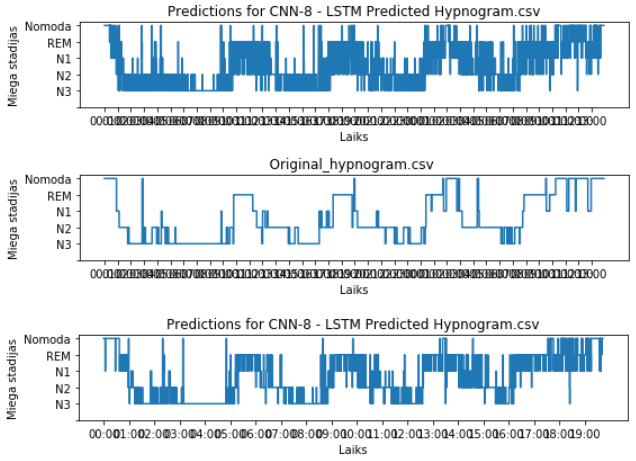
\includegraphics[width=1 \textwidth]{download123} 
\caption{Hipnogrammas}  \label{matmat} 
\end{figure}


\chapter*{Pārskats}
\addcontentsline{toc}{chapter}{Pārskats}

Darba laikā tika:
\begin{itemize}
\item Veikta miega fāžu izpēte, lai uzzinātu ar ko miega periodā katra fāze atšķiras un kādi viļņu paterni tiek novēroti. 
\item Apskatīti jau eksistējošie miega EEG signālu klasifikācijas projekti.
\item Izpētīti dziļās apmācības algoritmi. Vispirms CNN tad RNN un LSTM. Beigās tika apskatīts arī apvienotais CNN un LSTM modelis.
\item Veikta pieejamo miega EEG datubāžu izpēte, lai atrastu derīgas datubāzes, kas satur gan EDF failus gan to pavadošās hipnogrammas. 
\item Izpētīti risinājumi, kā veikt datu izguvi no EDF failiem un to pavadošajām hipnogrammām.
\item Apskatītas iespējamās izstrādes vides un modeļu izstrādes iespējas. Kā izstrādes vide tika izvēlēta Google Colab un kā programmēšanas valoda Python. Modeļu izstrādei tika izmantota Keras, kas ir atvērtā koda neironu tīkla bibliotēka, kas rakstīta Python.
\item Veikta datu kopas sagatavošana, kur no EDF failiem tika ņemti divu kanālu EEG signāli un pēc tam sadalīti ap apkašsignāliem, balstoties uz hipnogrammas miega fāžu sadalījumu.
\item Izveidots partijas ģenerators, kas tika izmantots tīkla apmācībā un validācijā.
\item Apmācītas četri modeļi uz divām klasēm (Nomoda un Miega) un pēc tam testēti. Iegūtie testēšanas rezultāti tika apvienoti kopējās tabulās un salīdzināti. 
\item Apmācītas četri modeļi uz 5 klasēm (Nomoda, N1,N2,N3 REM) un pēc tam testēti. Iegūtie testēšanas rezultāti tika apvienoti kopējās tabulās un salīdzināti. 
\
\end{itemize}

\chapter*{Secinājumi}
\addcontentsline{toc}{chapter}{Secinājumi}
\begin{itemize}
\item Dziļās apmācības metodes veiksmīgi spēj klasificēt Nomoda fāzi no miega fāzēm.
 \item Grūtības sagādā Nomoda fāzes atšķiršana no REM, kur REM varētu papildus noteikt, izmantojot elektromogrāfiju un acu artefaktu klātbūtnes noteikšanu, izmantojot papildus EEG sensorus. 
 \item LSTM nespēj veiksmīgi klasificēt datus, pārpratumu matricā uzrādot vāju klasificēšanas veiktspēju.
\item Nākošais solis būtu sagatavot datu kopu, kas saturētu tikai miega fāzes bez Nomoda fāzes, bet priekš tā dziļajām apmācības metodēm, ir nepieciešama daudz lielāka datu kopa.
\item Uz izvēlēto datu kopu, CNN apvienojot ar LSTM, izdevās iegūt labākus rezultātus nekā izmantojot katru tīklu arhitektūru atsevišķi.
\item 2 klašu gadījumā, kad datu izmērs ir 1000x2 modeļi spēj ļoti precīzi noteikt momentu, kad cilvēks ir aizmidzis. 
\item 2 klašu gadījumā Nomoda fāzi atšķirt no miega fāzes modeļiem sagādā lielāka grūtības, nekā atšķirt miega fāzes no Nomoda fāzes. 
\item N3 miega fāze visbiežāk tiek jaukta ar N2 fāzi, kā arī var secināt to, ka Nomoda fāze bieži tiek, uzskatīta par REM vai N1 staiju, jo tas ir moments, kas cilvēks vēl nav pilnībā aizmidzis. 
\item N3 un N2 ir fāzes, kuras modeļi spēj labāk atšķirt no citām fāzēm, jo šajās fāzēs cilvēks jau ir aizmidzis un viļņu paterni, kas rodas šo fāžu laikā ļoti atšķiras no REM, Nomoda un N1 fāzes. 
\item Darba laikā apskatītie projekti arī izmantoja to pašu datubāzi, kuru izvēlējās autore, jo ir piejamas, samēra maz miega EEG datu bāzes, kas iekļautu arī pavadošās hipnogrammas, kā arī datubāzes satur failus, kas nevienmēr ir EDF formātā.  
\end{itemize}

 

 %10 & 128 & 0.123 & 6.735 &-0.41923616  &0.11669113 \\
 %20 & 128 & 0.261 & 5.624 &0.03741  &0.33378655 \\
 %30 & 128 & 0.818 & 0.889 & 0.7652572  &0.69509822 \\
 %40 & 128 & 0.863 & 0.614 &0.79023569  &0.66687042 \\
 %50 & 128 & 0.87  & 0.638 & 0.8010683   & 0.02052493 \\
 %100 & 128 & 0.869 & 0.65 &0.80700118  &0.72770647 \\
 %\hline


    %\input{secinajumi-un-priesklikumi} %% Ērtāk visu failā secinajumi-un-priesklikumi.tex
    %% Nenumurēta nodaļa, kas uzrādās satura rādītājā
    
    \chapter*{Izmantotās literatūras un avotu saraksts}
    
    \title{References}
    \begingroup
       \def\chapter*#1{}
       \addcontentsline{toc}{chapter}{Izmantotās literatūras un avotu saraksts}
    \bibliography{bib/library}
    \bibliographystyle{IEEEtran}
    \endgroup
    
    % \printbibliography[title={Reference}]
    %\printbibliography
\appendix
\chapter*{Pielikumi}
\addcontentsline{toc}{chapter}{Pielikumi}

\section*{1. CNN-2 - LSTM iegūtie svari}
\addtocounter{nofappendices}{1}
Darknet ietvarā iegūtie svari atrodas \path{CNN2LSTM_weights} mapē.

\section*{2. CNN-8 - LSTM iegūtie svari}
\addtocounter{nofappendices}{1}
Visi mxnet-ssd ietvarā iegūtie svari atrodas \path{CNN8LSTM_weights} mapē.

\section*{3. CNN iegūtie svari}
\addtocounter{nofappendices}{1}
Visi mxnet-ssd ietvarā iegūtie svari atrodas \path{CNN_weights} mapē.

\section*{4. LSTM iegūtie svari}
\addtocounter{nofappendices}{1}
Visi mxnet-ssd ietvarā iegūtie svari atrodas \path{LSTM_weights} mapē.

\section*{5. Izmantotās apmācības un validācijas datu kopas}
\addtocounter{nofappendices}{1}
Izmantotās apmācības un validācijas datu kopas atrodas \path{sleep_edf} mapē.

\section*{6. Python piezīmju grāmatas fails SleepEEGClassification.ipynb}
\addtocounter{nofappendices}{1}
Izejas koda fails atrodas \path{SleepEEG} mapē.

%\section*{7. Klašu $F_1$ novērtējumi pie datu izmēra 500x2}
%
%\begin{table}[H]
%\centering
%\caption{}
%\captionsetup{justification=centering}
%\caption*{\textbf{Klašu $F_1$ novērtējumi}}
%\begin{tabular}{@{}lllllll@{}}
%%\hline
%\multicolumn{1}{c|}{Method} & \multicolumn{1}{c|}{Epoha} & %\multicolumn{1}{c}{Nomoda} & \multicolumn{1}{c}{REM} & \multicolumn{1}{c}{N1} & \multicolumn{1}{c}{N2} & \multicolumn{1}{c}{N3} \\ \hline
%\multicolumn{1}{l|}{LSTM} & \multicolumn{1}{c|}{\multirow{4}{*}{50}} & 0.07 & 0.16 & 0.11 & 0.28 & 0.23 \\
%\multicolumn{1}{l|}{CNN} & \multicolumn{1}{c|}{} & 0.48 & 0.44 & 0.19 & 0.59 & 0.68 \\
%\multicolumn{1}{l|}{CNN2-LSTM} & \multicolumn{1}{c|}{} & 0.40 & 0.17 & 0.20 & 0.60 & 0.69 \\
%\multicolumn{1}{l|}{CNN8-LSTM} & \multicolumn{1}{c|}{}& 0.45 & 0.47 & 0.19 & 0.48  & 0.69 \\ %\hline
%\multicolumn{1}{l|}{LSTM} & \multicolumn{1}{l|}{\multirow{4}{*}{30}} & 0.12 & 0.23 & 0.09 & 0.29 & 0.23 \\
%\multicolumn{1}{l|}{CNN} & \multicolumn{1}{l|}{} & \cellcolor[HTML]{FFCB2F}\textbf{0.53} & 0.40 & \cellcolor[HTML]{32CB00}\textbf{0.16} &  \cellcolor[HTML]{00D2CB}\textbf{0.66} & 0.75 \\
%\multicolumn{1}{l|}{CNN2-LSTM} & \multicolumn{1}{l|}{} & 0.52 & \cellcolor[HTML]{FAABF3}\textbf{0.53} & 0.02 & 0.61 & \cellcolor[HTML]{FD6864}\textbf{0.79} \\
%\multicolumn{1}{l|}{CNN8-LSTM} & \multicolumn{1}{l|}{} & 0.45 & 0.29 & 0.22 & 0.47 & 0.69 \\ \hline
%\end{tabular}
%\label{classF1Score}
%\end{table}

%\section*{8. Klašu $F_1$ novērtējumi}

%\begin{table}[H]
%\centering
%\caption{}
%\captionsetup{justification=centering}
%\caption*{\textbf{Klašu $F_1$ novērtējumi}}
%\begin{tabular}{l|l|lllll}
%\hline
%\multicolumn{1}{c|}{Method} & \multicolumn{1}{c|}{Epoch} & \multicolumn{1}{c}{Nomoda} & \multicolumn{1}{c}{REM} & \multicolumn{1}{c}{N1} & \multicolumn{1}{c}{N2} & \multicolumn{1}{c}{N3} \\ \hline
%CNN & \multirow{3}{*}{50} & 0.45 & 0.46 & 0.24 & 0.62 & 0.78 \\
%CNN2-LSTM &  & 0.41 & 0.21 & 0.24 & 0.35 & 0.71 \\
%CNN8-LSTM &  & 0.53 & 0.42 & 0.22 & 0.66 & 0.80 \\ \hline
%CNN & \multirow{3}{*}{100} & \cellcolor[HTML]{FFCB2F} \textbf{0.55} & 0.45 & 0.21 & 0.53 & 0.78 \\
%CNN2-LSTM &  & 0.39 & 0.26 & 0.21 & 0.46 & 0.73 \\
%CNN8-LSTM &  & \cellcolor[HTML]{FFCB2F} \textbf{0.55} & \cellcolor[HTML]{FAABF3} \textbf{0.57} & \cellcolor[HTML]{32CB00}\textbf{0.25} & \cellcolor[HTML]{00D2CB}\textbf{0.69} & \cellcolor[HTML]{FD6864}\textbf{0.80} \\ \hline
%\end{tabular}
%\label{optiClassRest2v}
%\end{table}



\chapter*{Galvojums}
\addcontentsline{toc}{chapter}{Galvojums}
Ar šo es, \defAutors , galvoju, ka maģistra darbs ir izpildīts patstāvīgi,
konsultējoties ar darba vadītāju. No svešiem pirmavotiem ņemtā informācija ir
norādīta ar atsaucēm, dati un definējumi ir uzrādīti darbā. Šis darbs tādā vai citādā veidā
nav nekad iesniegts nevienai citai pārbaudījumu komisijai.

Esmu informēts, ka mans maģistra darbs tiks ievietots un apstrādāts
Vienotajā datorizētajā plaģiāta kontroles sistēmā plāģiāta kontroles nolūkos.

\vspace{1in}
% \defGads.gada \rule{1cm}{0.2pt}\hspace{3mm}\rule{3cm}{0.2pt}
\begin{tabular}{@{}r@{}l@{}}
  \parbox[c]{0.7\textwidth}{\defGads.gada \rule{1cm}{0.2pt}\hspace{3mm}\rule{3cm}{0.2pt}}&
  \parbox[t]{0.2\textwidth}{\centering
  \mbox{}\hrulefill\vspace{-0.8em}\\
  {\scriptsize(paraksts)}\vspace{2em}}
\end{tabular}

Es, \defAutors , atļauju Ventspils Augstskolai savu maģistra darbu bez atlīdzības ievietot un 
uzglabāt Latvijas Nacionālās bibliotēkas pārvaldītā datortīklā Academia (www.academia.lndb.lv), 
kurā tie ir pieejami gan bibliotēkas lietotājiem, gan globālajā tīmeklī tādā veidā, 
ka ikviens tiem var piekļūt individuāli izraudzītā laikā, individuāli izraudzītā vietā.

\vspace{1in}
% \defGads.gada \rule{1cm}{0.2pt}\hspace{3mm}\rule{3cm}{0.2pt}
\begin{tabular}{@{}r@{}l@{}}
  \parbox[c]{0.7\textwidth}{} Piekrītu \rule{1cm}{0.2pt}&
  \parbox[t]{0.2\textwidth}{\centering
  \mbox{}\hrulefill\vspace{-0.8em}\\
  {}\vspace{2em}}\\

  \parbox[c]{0.7\textwidth}{} Nepiekrītu \rule{1cm}{0.2pt}&
   \parbox[t]{0.2\textwidth}{ \centering
  \mbox{}\hrulefill\vspace{-0.8em}\\
  {}\vspace{2em}}\\
  
  \parbox[c]{0.7\textwidth}{\defGads.gada \rule{1cm}{0.2pt}\hspace{3mm}\rule{3cm}{0.2pt}}&
\end{tabular}

\label{LastPage}
    
    \end{document}

